\documentclass[twoside]{book}

% Packages required by doxygen
\usepackage{fixltx2e}
\usepackage{calc}
\usepackage{doxygen}
\usepackage[export]{adjustbox} % also loads graphicx
\usepackage{graphicx}
\usepackage[utf8]{inputenc}
\usepackage{makeidx}
\usepackage{multicol}
\usepackage{multirow}
\PassOptionsToPackage{warn}{textcomp}
\usepackage{textcomp}
\usepackage[nointegrals]{wasysym}
\usepackage[table]{xcolor}

% Font selection
\usepackage[T1]{fontenc}
\usepackage[scaled=.90]{helvet}
\usepackage{courier}
\usepackage{amssymb}
\usepackage{sectsty}
\renewcommand{\familydefault}{\sfdefault}
\allsectionsfont{%
  \fontseries{bc}\selectfont%
  \color{darkgray}%
}
\renewcommand{\DoxyLabelFont}{%
  \fontseries{bc}\selectfont%
  \color{darkgray}%
}
\newcommand{\+}{\discretionary{\mbox{\scriptsize$\hookleftarrow$}}{}{}}

% Page & text layout
\usepackage{geometry}
\geometry{%
  a4paper,%
  top=2.5cm,%
  bottom=2.5cm,%
  left=2.5cm,%
  right=2.5cm%
}
\tolerance=750
\hfuzz=15pt
\hbadness=750
\setlength{\emergencystretch}{15pt}
\setlength{\parindent}{0cm}
\setlength{\parskip}{3ex plus 2ex minus 2ex}
\makeatletter
\renewcommand{\paragraph}{%
  \@startsection{paragraph}{4}{0ex}{-1.0ex}{1.0ex}{%
    \normalfont\normalsize\bfseries\SS@parafont%
  }%
}
\renewcommand{\subparagraph}{%
  \@startsection{subparagraph}{5}{0ex}{-1.0ex}{1.0ex}{%
    \normalfont\normalsize\bfseries\SS@subparafont%
  }%
}
\makeatother

% Headers & footers
\usepackage{fancyhdr}
\pagestyle{fancyplain}
\fancyhead[LE]{\fancyplain{}{\bfseries\thepage}}
\fancyhead[CE]{\fancyplain{}{}}
\fancyhead[RE]{\fancyplain{}{\bfseries\leftmark}}
\fancyhead[LO]{\fancyplain{}{\bfseries\rightmark}}
\fancyhead[CO]{\fancyplain{}{}}
\fancyhead[RO]{\fancyplain{}{\bfseries\thepage}}
\fancyfoot[LE]{\fancyplain{}{}}
\fancyfoot[CE]{\fancyplain{}{}}
\fancyfoot[RE]{\fancyplain{}{\bfseries\scriptsize Generated by Doxygen }}
\fancyfoot[LO]{\fancyplain{}{\bfseries\scriptsize Generated by Doxygen }}
\fancyfoot[CO]{\fancyplain{}{}}
\fancyfoot[RO]{\fancyplain{}{}}
\renewcommand{\footrulewidth}{0.4pt}
\renewcommand{\chaptermark}[1]{%
  \markboth{#1}{}%
}
\renewcommand{\sectionmark}[1]{%
  \markright{\thesection\ #1}%
}

% Indices & bibliography
\usepackage{natbib}
\usepackage[titles]{tocloft}
\setcounter{tocdepth}{3}
\setcounter{secnumdepth}{5}
\makeindex

% Hyperlinks (required, but should be loaded last)
\usepackage{ifpdf}
\ifpdf
  \usepackage[pdftex,pagebackref=true]{hyperref}
\else
  \usepackage[ps2pdf,pagebackref=true]{hyperref}
\fi
\hypersetup{%
  colorlinks=true,%
  linkcolor=blue,%
  citecolor=blue,%
  unicode%
}

% Custom commands
\newcommand{\clearemptydoublepage}{%
  \newpage{\pagestyle{empty}\cleardoublepage}%
}

\usepackage{caption}
\captionsetup{labelsep=space,justification=centering,font={bf},singlelinecheck=off,skip=4pt,position=top}

%===== C O N T E N T S =====

\begin{document}

% Titlepage & ToC
\hypersetup{pageanchor=false,
             bookmarksnumbered=true,
             pdfencoding=unicode
            }
\pagenumbering{alph}
\begin{titlepage}
\vspace*{7cm}
\begin{center}%
{\Large C\+AL v2 }\\
\vspace*{1cm}
{\large Generated by Doxygen 1.8.13}\\
\end{center}
\end{titlepage}
\clearemptydoublepage
\pagenumbering{roman}
\tableofcontents
\clearemptydoublepage
\pagenumbering{arabic}
\hypersetup{pageanchor=true}

%--- Begin generated contents ---
\chapter{Hierarchical Index}
\section{Class Hierarchy}
This inheritance list is sorted roughly, but not completely, alphabetically\+:\begin{DoxyCompactList}
\item \contentsline{section}{Aux\+Edge}{\pageref{class_aux_edge}}{}
\item \contentsline{section}{Camiao}{\pageref{class_camiao}}{}
\item \contentsline{section}{Comparison\+Market\+Similarity}{\pageref{class_comparison_market_similarity}}{}
\item \contentsline{section}{Comparison\+Request\+Distance}{\pageref{class_comparison_request_distance}}{}
\item \contentsline{section}{Comparison\+Request\+Size}{\pageref{class_comparison_request_size}}{}
\item \contentsline{section}{Comparison\+Street\+Similarity}{\pageref{class_comparison_street_similarity}}{}
\item \contentsline{section}{Edge$<$ T $>$}{\pageref{class_edge}}{}
\item \contentsline{section}{Graph$<$ T $>$}{\pageref{class_graph}}{}
\item \contentsline{section}{Graph$<$ Node\+Object $\ast$$>$}{\pageref{class_graph}}{}
\item \contentsline{section}{Menu}{\pageref{class_menu}}{}
\item \contentsline{section}{Node\+Object}{\pageref{class_node_object}}{}
\begin{DoxyCompactList}
\item \contentsline{section}{Client}{\pageref{class_client}}{}
\item \contentsline{section}{Supermercado}{\pageref{class_supermercado}}{}
\end{DoxyCompactList}
\item \contentsline{section}{Pedido}{\pageref{class_pedido}}{}
\item \contentsline{section}{Supermarket\+Manager}{\pageref{class_supermarket_manager}}{}
\item \contentsline{section}{Vertex$<$ T $>$}{\pageref{class_vertex}}{}
\end{DoxyCompactList}

\chapter{Class Index}
\section{Class List}
Here are the classes, structs, unions and interfaces with brief descriptions\+:\begin{DoxyCompactList}
\item\contentsline{section}{\hyperlink{class_aux_edge}{Aux\+Edge} }{\pageref{class_aux_edge}}{}
\item\contentsline{section}{\hyperlink{class_camiao}{Camiao} }{\pageref{class_camiao}}{}
\item\contentsline{section}{\hyperlink{class_client}{Client} }{\pageref{class_client}}{}
\item\contentsline{section}{\hyperlink{class_comparison_market_similarity}{Comparison\+Market\+Similarity} }{\pageref{class_comparison_market_similarity}}{}
\item\contentsline{section}{\hyperlink{class_comparison_request_distance}{Comparison\+Request\+Distance} }{\pageref{class_comparison_request_distance}}{}
\item\contentsline{section}{\hyperlink{class_comparison_request_size}{Comparison\+Request\+Size} }{\pageref{class_comparison_request_size}}{}
\item\contentsline{section}{\hyperlink{class_comparison_street_similarity}{Comparison\+Street\+Similarity} }{\pageref{class_comparison_street_similarity}}{}
\item\contentsline{section}{\hyperlink{class_edge}{Edge$<$ T $>$} }{\pageref{class_edge}}{}
\item\contentsline{section}{\hyperlink{class_graph}{Graph$<$ T $>$} }{\pageref{class_graph}}{}
\item\contentsline{section}{\hyperlink{class_menu}{Menu} }{\pageref{class_menu}}{}
\item\contentsline{section}{\hyperlink{class_node_object}{Node\+Object} }{\pageref{class_node_object}}{}
\item\contentsline{section}{\hyperlink{class_pedido}{Pedido} }{\pageref{class_pedido}}{}
\item\contentsline{section}{\hyperlink{class_supermarket_manager}{Supermarket\+Manager} }{\pageref{class_supermarket_manager}}{}
\item\contentsline{section}{\hyperlink{class_supermercado}{Supermercado} }{\pageref{class_supermercado}}{}
\item\contentsline{section}{\hyperlink{class_vertex}{Vertex$<$ T $>$} }{\pageref{class_vertex}}{}
\end{DoxyCompactList}

\chapter{File Index}
\section{File List}
Here is a list of all files with brief descriptions\+:\begin{DoxyCompactList}
\item\contentsline{section}{\hyperlink{_camiao_8cpp}{Camiao.\+cpp} }{\pageref{_camiao_8cpp}}{}
\item\contentsline{section}{\hyperlink{_camiao_8h}{Camiao.\+h} }{\pageref{_camiao_8h}}{}
\item\contentsline{section}{\hyperlink{_client_8cpp}{Client.\+cpp} }{\pageref{_client_8cpp}}{}
\item\contentsline{section}{\hyperlink{_client_8h}{Client.\+h} }{\pageref{_client_8h}}{}
\item\contentsline{section}{\hyperlink{_graph_8h}{Graph.\+h} }{\pageref{_graph_8h}}{}
\item\contentsline{section}{\hyperlink{_menu_8cpp}{Menu.\+cpp} }{\pageref{_menu_8cpp}}{}
\item\contentsline{section}{\hyperlink{_menu_8h}{Menu.\+h} }{\pageref{_menu_8h}}{}
\item\contentsline{section}{\hyperlink{_node_object_8cpp}{Node\+Object.\+cpp} }{\pageref{_node_object_8cpp}}{}
\item\contentsline{section}{\hyperlink{_node_object_8h}{Node\+Object.\+h} }{\pageref{_node_object_8h}}{}
\item\contentsline{section}{\hyperlink{_pedido_8h}{Pedido.\+h} }{\pageref{_pedido_8h}}{}
\item\contentsline{section}{\hyperlink{_source_8cpp}{Source.\+cpp} }{\pageref{_source_8cpp}}{}
\item\contentsline{section}{\hyperlink{_supermarket_manager_8cpp}{Supermarket\+Manager.\+cpp} }{\pageref{_supermarket_manager_8cpp}}{}
\item\contentsline{section}{\hyperlink{_supermarket_manager_8h}{Supermarket\+Manager.\+h} }{\pageref{_supermarket_manager_8h}}{}
\item\contentsline{section}{\hyperlink{_supermercado_8cpp}{Supermercado.\+cpp} }{\pageref{_supermercado_8cpp}}{}
\item\contentsline{section}{\hyperlink{_supermercado_8h}{Supermercado.\+h} }{\pageref{_supermercado_8h}}{}
\item\contentsline{section}{\hyperlink{_utils_8cpp}{Utils.\+cpp} }{\pageref{_utils_8cpp}}{}
\item\contentsline{section}{\hyperlink{_utils_8h}{Utils.\+h} }{\pageref{_utils_8h}}{}
\end{DoxyCompactList}

\chapter{Class Documentation}
\hypertarget{class_aux_edge}{}\section{Aux\+Edge Class Reference}
\label{class_aux_edge}\index{Aux\+Edge@{Aux\+Edge}}


{\ttfamily \#include $<$Utils.\+h$>$}

\subsection*{Public Member Functions}
\begin{DoxyCompactItemize}
\item 
\hyperlink{class_aux_edge_aff00b230c80f8b62dca6ed5d1d4baaf9}{Aux\+Edge} ()
\item 
\hyperlink{class_aux_edge_ab937368463372c5f87c1805f46318b5a}{Aux\+Edge} (int \hyperlink{class_aux_edge_ae60cad09cc21dd040c40d81139dbc2e7}{src}, int \hyperlink{class_aux_edge_acee560d785382eeb7ed695c59903bbe9}{dest}, int \hyperlink{class_aux_edge_a688348db28aaaea42d86ea26f33177b2}{w}, string \hyperlink{class_aux_edge_a7a52a82fb74a6eddcdab0d4d45917767}{rua}, string \hyperlink{class_aux_edge_aa9a8ff092babb6f3e3df271b400cdf17}{distrito})
\item 
bool \hyperlink{class_aux_edge_ac5b9bcaa74464f7a5e79ec56d4c87b0d}{operator==} (const \hyperlink{class_aux_edge}{Aux\+Edge} \&rhs)
\item 
bool \hyperlink{class_aux_edge_ac05b44fbcf9e494b0d92df6359ac9932}{exists} (vector$<$ \hyperlink{class_aux_edge}{Aux\+Edge} $>$ edges)
\item 
\hyperlink{class_aux_edge}{Aux\+Edge} \hyperlink{class_aux_edge_a6561f80676278a04d73640c2166c438f}{reverse} ()
\end{DoxyCompactItemize}
\subsection*{Public Attributes}
\begin{DoxyCompactItemize}
\item 
int \hyperlink{class_aux_edge_ae60cad09cc21dd040c40d81139dbc2e7}{src}
\item 
int \hyperlink{class_aux_edge_acee560d785382eeb7ed695c59903bbe9}{dest}
\item 
int \hyperlink{class_aux_edge_a688348db28aaaea42d86ea26f33177b2}{w}
\item 
string \hyperlink{class_aux_edge_a7a52a82fb74a6eddcdab0d4d45917767}{rua}
\item 
string \hyperlink{class_aux_edge_aa9a8ff092babb6f3e3df271b400cdf17}{distrito}
\end{DoxyCompactItemize}


\subsection{Constructor \& Destructor Documentation}
\mbox{\Hypertarget{class_aux_edge_aff00b230c80f8b62dca6ed5d1d4baaf9}\label{class_aux_edge_aff00b230c80f8b62dca6ed5d1d4baaf9}} 
\index{Aux\+Edge@{Aux\+Edge}!Aux\+Edge@{Aux\+Edge}}
\index{Aux\+Edge@{Aux\+Edge}!Aux\+Edge@{Aux\+Edge}}
\subsubsection{\texorpdfstring{Aux\+Edge()}{AuxEdge()}\hspace{0.1cm}{\footnotesize\ttfamily [1/2]}}
{\footnotesize\ttfamily Aux\+Edge\+::\+Aux\+Edge (\begin{DoxyParamCaption}{ }\end{DoxyParamCaption})\hspace{0.3cm}{\ttfamily [inline]}}

Construtor por omissao. \mbox{\Hypertarget{class_aux_edge_ab937368463372c5f87c1805f46318b5a}\label{class_aux_edge_ab937368463372c5f87c1805f46318b5a}} 
\index{Aux\+Edge@{Aux\+Edge}!Aux\+Edge@{Aux\+Edge}}
\index{Aux\+Edge@{Aux\+Edge}!Aux\+Edge@{Aux\+Edge}}
\subsubsection{\texorpdfstring{Aux\+Edge()}{AuxEdge()}\hspace{0.1cm}{\footnotesize\ttfamily [2/2]}}
{\footnotesize\ttfamily Aux\+Edge\+::\+Aux\+Edge (\begin{DoxyParamCaption}\item[{int}]{src,  }\item[{int}]{dest,  }\item[{int}]{w,  }\item[{string}]{rua,  }\item[{string}]{distrito }\end{DoxyParamCaption})\hspace{0.3cm}{\ttfamily [inline]}}

Construtor que atribui valores aos atributos da classe.


\begin{DoxyParams}{Parameters}
{\em src} & fonte da aresta \\
\hline
{\em dest} & destino da aresta \\
\hline
{\em w} & peso da aresta \\
\hline
{\em rua} & rua da aresta \\
\hline
{\em distrito} & distrito da aresta \\
\hline
\end{DoxyParams}


\subsection{Member Function Documentation}
\mbox{\Hypertarget{class_aux_edge_ac05b44fbcf9e494b0d92df6359ac9932}\label{class_aux_edge_ac05b44fbcf9e494b0d92df6359ac9932}} 
\index{Aux\+Edge@{Aux\+Edge}!exists@{exists}}
\index{exists@{exists}!Aux\+Edge@{Aux\+Edge}}
\subsubsection{\texorpdfstring{exists()}{exists()}}
{\footnotesize\ttfamily bool Aux\+Edge\+::exists (\begin{DoxyParamCaption}\item[{vector$<$ \hyperlink{class_aux_edge}{Aux\+Edge} $>$}]{edges }\end{DoxyParamCaption})\hspace{0.3cm}{\ttfamily [inline]}}

Funcao que indica se esta \hyperlink{class_aux_edge}{Aux\+Edge} existe no vetor dado.


\begin{DoxyParams}{Parameters}
{\em edges} & vetor de Aux\+Edges \\
\hline
\end{DoxyParams}
\begin{DoxyReturn}{Returns}
true se esta \hyperlink{class_aux_edge}{Aux\+Edge} existe no vetor dado e false caso contrario 
\end{DoxyReturn}
Here is the caller graph for this function\+:
\nopagebreak
\begin{figure}[H]
\begin{center}
\leavevmode
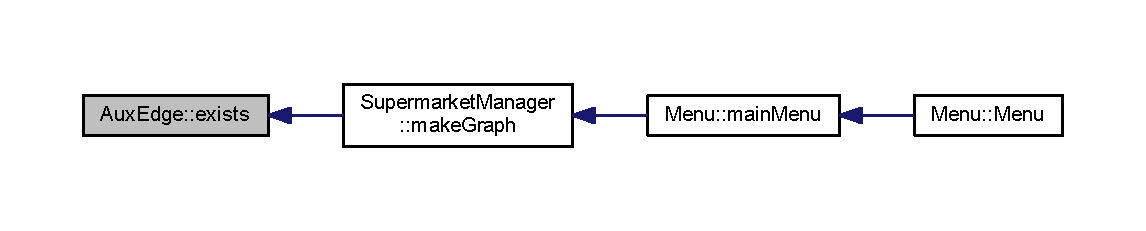
\includegraphics[width=350pt]{class_aux_edge_ac05b44fbcf9e494b0d92df6359ac9932_icgraph}
\end{center}
\end{figure}
\mbox{\Hypertarget{class_aux_edge_ac5b9bcaa74464f7a5e79ec56d4c87b0d}\label{class_aux_edge_ac5b9bcaa74464f7a5e79ec56d4c87b0d}} 
\index{Aux\+Edge@{Aux\+Edge}!operator==@{operator==}}
\index{operator==@{operator==}!Aux\+Edge@{Aux\+Edge}}
\subsubsection{\texorpdfstring{operator==()}{operator==()}}
{\footnotesize\ttfamily bool Aux\+Edge\+::operator== (\begin{DoxyParamCaption}\item[{const \hyperlink{class_aux_edge}{Aux\+Edge} \&}]{rhs }\end{DoxyParamCaption})\hspace{0.3cm}{\ttfamily [inline]}}

Operador de igualdade desta classe. Duas \hyperlink{class_aux_edge}{Aux\+Edge} sao iguais se tiverem a mesma fonte e destino ou tiverem a mesma rua.


\begin{DoxyParams}{Parameters}
{\em rhs} & \hyperlink{class_aux_edge}{Aux\+Edge} a comparar \\
\hline
\end{DoxyParams}
\begin{DoxyReturn}{Returns}
true se as \hyperlink{class_aux_edge}{Aux\+Edge} sao iguais e false caso contrario 
\end{DoxyReturn}
\mbox{\Hypertarget{class_aux_edge_a6561f80676278a04d73640c2166c438f}\label{class_aux_edge_a6561f80676278a04d73640c2166c438f}} 
\index{Aux\+Edge@{Aux\+Edge}!reverse@{reverse}}
\index{reverse@{reverse}!Aux\+Edge@{Aux\+Edge}}
\subsubsection{\texorpdfstring{reverse()}{reverse()}}
{\footnotesize\ttfamily \hyperlink{class_aux_edge}{Aux\+Edge} Aux\+Edge\+::reverse (\begin{DoxyParamCaption}{ }\end{DoxyParamCaption})\hspace{0.3cm}{\ttfamily [inline]}}

Funcao que troca o sentido de uma \hyperlink{class_aux_edge}{Aux\+Edge}.

\begin{DoxyReturn}{Returns}
\hyperlink{class_aux_edge}{Aux\+Edge} com o sentido trocado. 
\end{DoxyReturn}


\subsection{Member Data Documentation}
\mbox{\Hypertarget{class_aux_edge_acee560d785382eeb7ed695c59903bbe9}\label{class_aux_edge_acee560d785382eeb7ed695c59903bbe9}} 
\index{Aux\+Edge@{Aux\+Edge}!dest@{dest}}
\index{dest@{dest}!Aux\+Edge@{Aux\+Edge}}
\subsubsection{\texorpdfstring{dest}{dest}}
{\footnotesize\ttfamily int Aux\+Edge\+::dest}

\mbox{\Hypertarget{class_aux_edge_aa9a8ff092babb6f3e3df271b400cdf17}\label{class_aux_edge_aa9a8ff092babb6f3e3df271b400cdf17}} 
\index{Aux\+Edge@{Aux\+Edge}!distrito@{distrito}}
\index{distrito@{distrito}!Aux\+Edge@{Aux\+Edge}}
\subsubsection{\texorpdfstring{distrito}{distrito}}
{\footnotesize\ttfamily string Aux\+Edge\+::distrito}

\mbox{\Hypertarget{class_aux_edge_a7a52a82fb74a6eddcdab0d4d45917767}\label{class_aux_edge_a7a52a82fb74a6eddcdab0d4d45917767}} 
\index{Aux\+Edge@{Aux\+Edge}!rua@{rua}}
\index{rua@{rua}!Aux\+Edge@{Aux\+Edge}}
\subsubsection{\texorpdfstring{rua}{rua}}
{\footnotesize\ttfamily string Aux\+Edge\+::rua}

Rua e distrito da aresta. \mbox{\Hypertarget{class_aux_edge_ae60cad09cc21dd040c40d81139dbc2e7}\label{class_aux_edge_ae60cad09cc21dd040c40d81139dbc2e7}} 
\index{Aux\+Edge@{Aux\+Edge}!src@{src}}
\index{src@{src}!Aux\+Edge@{Aux\+Edge}}
\subsubsection{\texorpdfstring{src}{src}}
{\footnotesize\ttfamily int Aux\+Edge\+::src}

Fonte, destino e peso da aresta. \mbox{\Hypertarget{class_aux_edge_a688348db28aaaea42d86ea26f33177b2}\label{class_aux_edge_a688348db28aaaea42d86ea26f33177b2}} 
\index{Aux\+Edge@{Aux\+Edge}!w@{w}}
\index{w@{w}!Aux\+Edge@{Aux\+Edge}}
\subsubsection{\texorpdfstring{w}{w}}
{\footnotesize\ttfamily int Aux\+Edge\+::w}



The documentation for this class was generated from the following file\+:\begin{DoxyCompactItemize}
\item 
\hyperlink{_utils_8h}{Utils.\+h}\end{DoxyCompactItemize}

\hypertarget{class_camiao}{}\section{Camiao Class Reference}
\label{class_camiao}\index{Camiao@{Camiao}}


{\ttfamily \#include $<$Camiao.\+h$>$}

\subsection*{Public Member Functions}
\begin{DoxyCompactItemize}
\item 
\hyperlink{class_camiao_a8924e9cf4f02c60f1233599c891a5f03}{Camiao} ()
\item 
void \hyperlink{class_camiao_a6b10fd5e1c3dc7e23236d9ac609adcc4}{reset} ()
\item 
void \hyperlink{class_camiao_a1425f4d0a4e86f9e41cd1c5320831cec}{add\+Pedido} (\hyperlink{class_pedido}{Pedido} $\ast$pedido)
\item 
int \hyperlink{class_camiao_af1ddc476c31697269601a7385a07e95f}{get\+Capacidade\+Usada} ()
\item 
int \hyperlink{class_camiao_ad30eac198fbce433526d12da8b3dbab6}{get\+Capacidade\+Maxima} ()
\item 
int \hyperlink{class_camiao_a4921ceaf1c790339e83e2bcde913d6cc}{get\+Distance\+Covered} ()
\item 
void \hyperlink{class_camiao_a33ef278250ffa4137788a5f275cf1f4b}{add\+Distance} (int distance)
\item 
queue$<$ \hyperlink{class_pedido}{Pedido} $\ast$ $>$ \hyperlink{class_camiao_a4baf70f4627ed9bee652a86ec4fa70fe}{get\+Itenerario} ()
\item 
void \hyperlink{class_camiao_ad3081de0be4dfc4930b0cf674d3077d3}{print\+Itenerario} (int supermarket\+ID, int pos)
\end{DoxyCompactItemize}
\subsection*{Private Attributes}
\begin{DoxyCompactItemize}
\item 
const int \hyperlink{class_camiao_a937608cbcb0e0ce51f0f6868fafb9ce7}{capacidade\+Maxima} = 100
\item 
int \hyperlink{class_camiao_aa486e5371c70048c8a88046c1a39051c}{capacidade\+Usada} = 0
\item 
queue$<$ \hyperlink{class_pedido}{Pedido} $\ast$ $>$ \hyperlink{class_camiao_aed76aba216d57a69565d997ba5d2b8d3}{itenerario}
\item 
int \hyperlink{class_camiao_afba63d9fec7c2fef600e22240d414f75}{distance\+Covered} = 0
\end{DoxyCompactItemize}


\subsection{Constructor \& Destructor Documentation}
\mbox{\Hypertarget{class_camiao_a8924e9cf4f02c60f1233599c891a5f03}\label{class_camiao_a8924e9cf4f02c60f1233599c891a5f03}} 
\index{Camiao@{Camiao}!Camiao@{Camiao}}
\index{Camiao@{Camiao}!Camiao@{Camiao}}
\subsubsection{\texorpdfstring{Camiao()}{Camiao()}}
{\footnotesize\ttfamily Camiao\+::\+Camiao (\begin{DoxyParamCaption}{ }\end{DoxyParamCaption})\hspace{0.3cm}{\ttfamily [inline]}}

Construtor por omissao de um camiao. 

\subsection{Member Function Documentation}
\mbox{\Hypertarget{class_camiao_a33ef278250ffa4137788a5f275cf1f4b}\label{class_camiao_a33ef278250ffa4137788a5f275cf1f4b}} 
\index{Camiao@{Camiao}!add\+Distance@{add\+Distance}}
\index{add\+Distance@{add\+Distance}!Camiao@{Camiao}}
\subsubsection{\texorpdfstring{add\+Distance()}{addDistance()}}
{\footnotesize\ttfamily void Camiao\+::add\+Distance (\begin{DoxyParamCaption}\item[{int}]{distance }\end{DoxyParamCaption})\hspace{0.3cm}{\ttfamily [inline]}}

Adiciona uma distancia a distancia total percorrida pelo camiao


\begin{DoxyParams}{Parameters}
{\em distance} & distancia a adicionar \\
\hline
\end{DoxyParams}
\mbox{\Hypertarget{class_camiao_a1425f4d0a4e86f9e41cd1c5320831cec}\label{class_camiao_a1425f4d0a4e86f9e41cd1c5320831cec}} 
\index{Camiao@{Camiao}!add\+Pedido@{add\+Pedido}}
\index{add\+Pedido@{add\+Pedido}!Camiao@{Camiao}}
\subsubsection{\texorpdfstring{add\+Pedido()}{addPedido()}}
{\footnotesize\ttfamily void Camiao\+::add\+Pedido (\begin{DoxyParamCaption}\item[{\hyperlink{class_pedido}{Pedido} $\ast$}]{pedido }\end{DoxyParamCaption})\hspace{0.3cm}{\ttfamily [inline]}}

Adiciona um pedido ao itenerario a ser realizado pelo camiao. Atualiza a capacidade usada pelo camiao, somando-\/lhe o tamanho do pedido.


\begin{DoxyParams}{Parameters}
{\em pedido} & apontador para o pedido a adicionar ao camiao \\
\hline
\end{DoxyParams}
Here is the call graph for this function\+:
\nopagebreak
\begin{figure}[H]
\begin{center}
\leavevmode
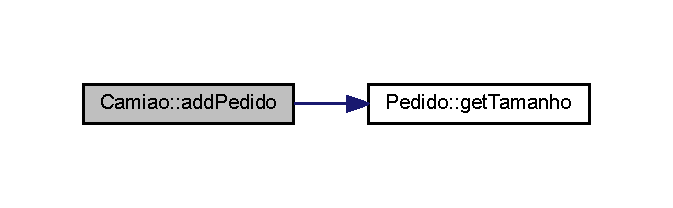
\includegraphics[width=323pt]{class_camiao_a1425f4d0a4e86f9e41cd1c5320831cec_cgraph}
\end{center}
\end{figure}
\mbox{\Hypertarget{class_camiao_ad30eac198fbce433526d12da8b3dbab6}\label{class_camiao_ad30eac198fbce433526d12da8b3dbab6}} 
\index{Camiao@{Camiao}!get\+Capacidade\+Maxima@{get\+Capacidade\+Maxima}}
\index{get\+Capacidade\+Maxima@{get\+Capacidade\+Maxima}!Camiao@{Camiao}}
\subsubsection{\texorpdfstring{get\+Capacidade\+Maxima()}{getCapacidadeMaxima()}}
{\footnotesize\ttfamily int Camiao\+::get\+Capacidade\+Maxima (\begin{DoxyParamCaption}{ }\end{DoxyParamCaption})\hspace{0.3cm}{\ttfamily [inline]}}

Retorna a capacidade maxima do camiao

\begin{DoxyReturn}{Returns}
a capacidade maxima do camiao 
\end{DoxyReturn}
\mbox{\Hypertarget{class_camiao_af1ddc476c31697269601a7385a07e95f}\label{class_camiao_af1ddc476c31697269601a7385a07e95f}} 
\index{Camiao@{Camiao}!get\+Capacidade\+Usada@{get\+Capacidade\+Usada}}
\index{get\+Capacidade\+Usada@{get\+Capacidade\+Usada}!Camiao@{Camiao}}
\subsubsection{\texorpdfstring{get\+Capacidade\+Usada()}{getCapacidadeUsada()}}
{\footnotesize\ttfamily int Camiao\+::get\+Capacidade\+Usada (\begin{DoxyParamCaption}{ }\end{DoxyParamCaption})\hspace{0.3cm}{\ttfamily [inline]}}

Retorna a capacidade atualmente usada pelo camiao

\begin{DoxyReturn}{Returns}
a capacidade atualmente usada pelo camiao 
\end{DoxyReturn}
\mbox{\Hypertarget{class_camiao_a4921ceaf1c790339e83e2bcde913d6cc}\label{class_camiao_a4921ceaf1c790339e83e2bcde913d6cc}} 
\index{Camiao@{Camiao}!get\+Distance\+Covered@{get\+Distance\+Covered}}
\index{get\+Distance\+Covered@{get\+Distance\+Covered}!Camiao@{Camiao}}
\subsubsection{\texorpdfstring{get\+Distance\+Covered()}{getDistanceCovered()}}
{\footnotesize\ttfamily int Camiao\+::get\+Distance\+Covered (\begin{DoxyParamCaption}{ }\end{DoxyParamCaption})\hspace{0.3cm}{\ttfamily [inline]}}

Retorna a distancia total percorrida no itenerario do camiao

\begin{DoxyReturn}{Returns}
a distancia total percorrida no itenerario do camiao 
\end{DoxyReturn}
Here is the caller graph for this function\+:
\nopagebreak
\begin{figure}[H]
\begin{center}
\leavevmode
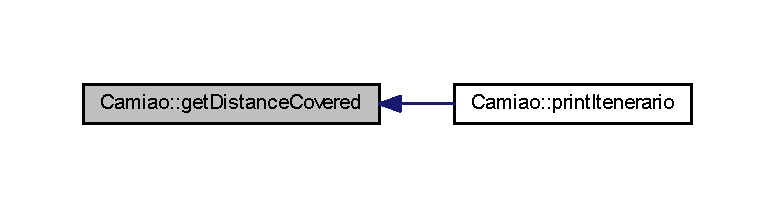
\includegraphics[width=350pt]{class_camiao_a4921ceaf1c790339e83e2bcde913d6cc_icgraph}
\end{center}
\end{figure}
\mbox{\Hypertarget{class_camiao_a4baf70f4627ed9bee652a86ec4fa70fe}\label{class_camiao_a4baf70f4627ed9bee652a86ec4fa70fe}} 
\index{Camiao@{Camiao}!get\+Itenerario@{get\+Itenerario}}
\index{get\+Itenerario@{get\+Itenerario}!Camiao@{Camiao}}
\subsubsection{\texorpdfstring{get\+Itenerario()}{getItenerario()}}
{\footnotesize\ttfamily queue$<$\hyperlink{class_pedido}{Pedido}$\ast$$>$ Camiao\+::get\+Itenerario (\begin{DoxyParamCaption}{ }\end{DoxyParamCaption})\hspace{0.3cm}{\ttfamily [inline]}}

Retorna o itenerario do camiao

\begin{DoxyReturn}{Returns}
o itenerario do camiao 
\end{DoxyReturn}
\mbox{\Hypertarget{class_camiao_ad3081de0be4dfc4930b0cf674d3077d3}\label{class_camiao_ad3081de0be4dfc4930b0cf674d3077d3}} 
\index{Camiao@{Camiao}!print\+Itenerario@{print\+Itenerario}}
\index{print\+Itenerario@{print\+Itenerario}!Camiao@{Camiao}}
\subsubsection{\texorpdfstring{print\+Itenerario()}{printItenerario()}}
{\footnotesize\ttfamily void Camiao\+::print\+Itenerario (\begin{DoxyParamCaption}\item[{int}]{supermarket\+ID,  }\item[{int}]{pos }\end{DoxyParamCaption})}

Imprime o itenerario do camiao de n�mero \textquotesingle{}pos\textquotesingle{} pertencente ao supermercado de ID \textquotesingle{}supermarket\+ID\textquotesingle{}. O ID de um supermercado � atribuido sequencialmente aquando da leitura do ficheiro do grafo. Cada supermercado tem um vetor de camioes, sendo o numero de cada camiao obtido somando 1 ao seu indice nesse vetor.


\begin{DoxyParams}{Parameters}
{\em supermarket\+ID} & ID do supermercado que possui este camiao \\
\hline
{\em pos} & numero deste camiao \\
\hline
\end{DoxyParams}
Here is the call graph for this function\+:
\nopagebreak
\begin{figure}[H]
\begin{center}
\leavevmode
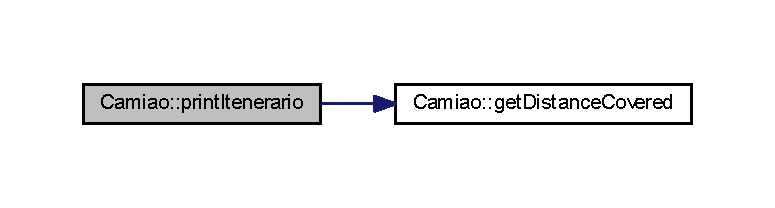
\includegraphics[width=350pt]{class_camiao_ad3081de0be4dfc4930b0cf674d3077d3_cgraph}
\end{center}
\end{figure}
\mbox{\Hypertarget{class_camiao_a6b10fd5e1c3dc7e23236d9ac609adcc4}\label{class_camiao_a6b10fd5e1c3dc7e23236d9ac609adcc4}} 
\index{Camiao@{Camiao}!reset@{reset}}
\index{reset@{reset}!Camiao@{Camiao}}
\subsubsection{\texorpdfstring{reset()}{reset()}}
{\footnotesize\ttfamily void Camiao\+::reset (\begin{DoxyParamCaption}{ }\end{DoxyParamCaption})\hspace{0.3cm}{\ttfamily [inline]}}

Coloca a zeros a capacidade usada e a distancia percorrida pelo camiao. 

\subsection{Member Data Documentation}
\mbox{\Hypertarget{class_camiao_a937608cbcb0e0ce51f0f6868fafb9ce7}\label{class_camiao_a937608cbcb0e0ce51f0f6868fafb9ce7}} 
\index{Camiao@{Camiao}!capacidade\+Maxima@{capacidade\+Maxima}}
\index{capacidade\+Maxima@{capacidade\+Maxima}!Camiao@{Camiao}}
\subsubsection{\texorpdfstring{capacidade\+Maxima}{capacidadeMaxima}}
{\footnotesize\ttfamily const int Camiao\+::capacidade\+Maxima = 100\hspace{0.3cm}{\ttfamily [private]}}

Capacidade de armazenamento maxima do camiao. Um camiao pode armazenar varios pedidos, tendo cada um deles um determinado tamanho. \mbox{\Hypertarget{class_camiao_aa486e5371c70048c8a88046c1a39051c}\label{class_camiao_aa486e5371c70048c8a88046c1a39051c}} 
\index{Camiao@{Camiao}!capacidade\+Usada@{capacidade\+Usada}}
\index{capacidade\+Usada@{capacidade\+Usada}!Camiao@{Camiao}}
\subsubsection{\texorpdfstring{capacidade\+Usada}{capacidadeUsada}}
{\footnotesize\ttfamily int Camiao\+::capacidade\+Usada = 0\hspace{0.3cm}{\ttfamily [private]}}

Capacidade que esta a ser usada pelo camiao, ou seja, a soma dos tamanhos dos pedidos armazenados pelo camiao neste momento. \mbox{\Hypertarget{class_camiao_afba63d9fec7c2fef600e22240d414f75}\label{class_camiao_afba63d9fec7c2fef600e22240d414f75}} 
\index{Camiao@{Camiao}!distance\+Covered@{distance\+Covered}}
\index{distance\+Covered@{distance\+Covered}!Camiao@{Camiao}}
\subsubsection{\texorpdfstring{distance\+Covered}{distanceCovered}}
{\footnotesize\ttfamily int Camiao\+::distance\+Covered = 0\hspace{0.3cm}{\ttfamily [private]}}

Distancia total percorrida pelo camiao no seu itenerario. \mbox{\Hypertarget{class_camiao_aed76aba216d57a69565d997ba5d2b8d3}\label{class_camiao_aed76aba216d57a69565d997ba5d2b8d3}} 
\index{Camiao@{Camiao}!itenerario@{itenerario}}
\index{itenerario@{itenerario}!Camiao@{Camiao}}
\subsubsection{\texorpdfstring{itenerario}{itenerario}}
{\footnotesize\ttfamily queue$<$\hyperlink{class_pedido}{Pedido}$\ast$$>$ Camiao\+::itenerario\hspace{0.3cm}{\ttfamily [private]}}



The documentation for this class was generated from the following files\+:\begin{DoxyCompactItemize}
\item 
\hyperlink{_camiao_8h}{Camiao.\+h}\item 
\hyperlink{_camiao_8cpp}{Camiao.\+cpp}\end{DoxyCompactItemize}

\hypertarget{class_client}{}\section{Client Class Reference}
\label{class_client}\index{Client@{Client}}


{\ttfamily \#include $<$Client.\+h$>$}



Inheritance diagram for Client\+:
\nopagebreak
\begin{figure}[H]
\begin{center}
\leavevmode
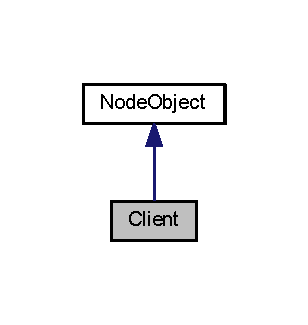
\includegraphics[width=148pt]{class_client__inherit__graph}
\end{center}
\end{figure}


Collaboration diagram for Client\+:
\nopagebreak
\begin{figure}[H]
\begin{center}
\leavevmode
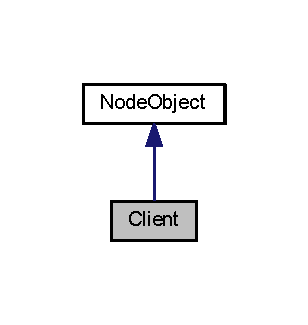
\includegraphics[width=148pt]{class_client__coll__graph}
\end{center}
\end{figure}
\subsection*{Public Member Functions}
\begin{DoxyCompactItemize}
\item 
\hyperlink{class_client_ae51af7aa6b8f591496a8f6a4a87a14bf}{Client} ()
\item 
void \hyperlink{class_client_acf31317770c47dc7087dceffe5663b73}{reset\+Id\+Counter} ()
\end{DoxyCompactItemize}
\subsection*{Additional Inherited Members}


\subsection{Constructor \& Destructor Documentation}
\mbox{\Hypertarget{class_client_ae51af7aa6b8f591496a8f6a4a87a14bf}\label{class_client_ae51af7aa6b8f591496a8f6a4a87a14bf}} 
\index{Client@{Client}!Client@{Client}}
\index{Client@{Client}!Client@{Client}}
\subsubsection{\texorpdfstring{Client()}{Client()}}
{\footnotesize\ttfamily Client\+::\+Client (\begin{DoxyParamCaption}{ }\end{DoxyParamCaption})}

Construtor por omissao de um cliente. 

\subsection{Member Function Documentation}
\mbox{\Hypertarget{class_client_acf31317770c47dc7087dceffe5663b73}\label{class_client_acf31317770c47dc7087dceffe5663b73}} 
\index{Client@{Client}!reset\+Id\+Counter@{reset\+Id\+Counter}}
\index{reset\+Id\+Counter@{reset\+Id\+Counter}!Client@{Client}}
\subsubsection{\texorpdfstring{reset\+Id\+Counter()}{resetIdCounter()}}
{\footnotesize\ttfamily void Client\+::reset\+Id\+Counter (\begin{DoxyParamCaption}{ }\end{DoxyParamCaption})}

Coloca a zero o contador sequencial de I\+Ds (dos clientes e supermercados). Here is the caller graph for this function\+:
\nopagebreak
\begin{figure}[H]
\begin{center}
\leavevmode
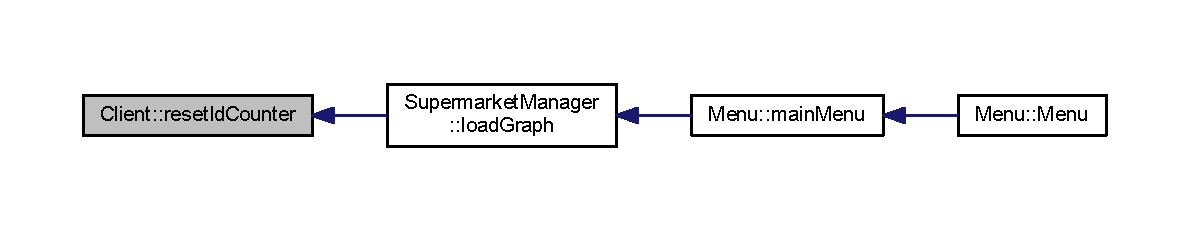
\includegraphics[width=350pt]{class_client_acf31317770c47dc7087dceffe5663b73_icgraph}
\end{center}
\end{figure}


The documentation for this class was generated from the following files\+:\begin{DoxyCompactItemize}
\item 
\hyperlink{_client_8h}{Client.\+h}\item 
\hyperlink{_client_8cpp}{Client.\+cpp}\end{DoxyCompactItemize}

\hypertarget{class_comparison_market_similarity}{}\section{Comparison\+Market\+Similarity Class Reference}
\label{class_comparison_market_similarity}\index{Comparison\+Market\+Similarity@{Comparison\+Market\+Similarity}}


{\ttfamily \#include $<$Utils.\+h$>$}

\subsection*{Public Member Functions}
\begin{DoxyCompactItemize}
\item 
bool \hyperlink{class_comparison_market_similarity_a9755661e6a4873505b4ec11935cb82a2}{operator()} (pair$<$ \hyperlink{class_node_object}{Node\+Object} $\ast$, int $>$ a, pair$<$ \hyperlink{class_node_object}{Node\+Object} $\ast$, int $>$ b)
\end{DoxyCompactItemize}


\subsection{Member Function Documentation}
\mbox{\Hypertarget{class_comparison_market_similarity_a9755661e6a4873505b4ec11935cb82a2}\label{class_comparison_market_similarity_a9755661e6a4873505b4ec11935cb82a2}} 
\index{Comparison\+Market\+Similarity@{Comparison\+Market\+Similarity}!operator()@{operator()}}
\index{operator()@{operator()}!Comparison\+Market\+Similarity@{Comparison\+Market\+Similarity}}
\subsubsection{\texorpdfstring{operator()()}{operator()()}}
{\footnotesize\ttfamily bool Comparison\+Market\+Similarity\+::operator() (\begin{DoxyParamCaption}\item[{pair$<$ \hyperlink{class_node_object}{Node\+Object} $\ast$, int $>$}]{a,  }\item[{pair$<$ \hyperlink{class_node_object}{Node\+Object} $\ast$, int $>$}]{b }\end{DoxyParamCaption})\hspace{0.3cm}{\ttfamily [inline]}}

Operador utilizado para a ordena��o da fila de prioridade markets da funcao approximate\+Search\+Supermarket, de modo a que a rua de maior similaridade esteja � cabe�a da fila. 

The documentation for this class was generated from the following file\+:\begin{DoxyCompactItemize}
\item 
\hyperlink{_utils_8h}{Utils.\+h}\end{DoxyCompactItemize}

\hypertarget{class_comparison_request_distance}{}\section{Comparison\+Request\+Distance Class Reference}
\label{class_comparison_request_distance}\index{Comparison\+Request\+Distance@{Comparison\+Request\+Distance}}


{\ttfamily \#include $<$Utils.\+h$>$}

\subsection*{Public Member Functions}
\begin{DoxyCompactItemize}
\item 
bool \hyperlink{class_comparison_request_distance_a8df25b4ebe4b2593e35d9ae8adba5f02}{operator()} (\hyperlink{class_pedido}{Pedido} $\ast$a, \hyperlink{class_pedido}{Pedido} $\ast$b)
\end{DoxyCompactItemize}


\subsection{Member Function Documentation}
\mbox{\Hypertarget{class_comparison_request_distance_a8df25b4ebe4b2593e35d9ae8adba5f02}\label{class_comparison_request_distance_a8df25b4ebe4b2593e35d9ae8adba5f02}} 
\index{Comparison\+Request\+Distance@{Comparison\+Request\+Distance}!operator()@{operator()}}
\index{operator()@{operator()}!Comparison\+Request\+Distance@{Comparison\+Request\+Distance}}
\subsubsection{\texorpdfstring{operator()()}{operator()()}}
{\footnotesize\ttfamily bool Comparison\+Request\+Distance\+::operator() (\begin{DoxyParamCaption}\item[{\hyperlink{class_pedido}{Pedido} $\ast$}]{a,  }\item[{\hyperlink{class_pedido}{Pedido} $\ast$}]{b }\end{DoxyParamCaption})\hspace{0.3cm}{\ttfamily [inline]}}

Operador utilizado para a ordena��o da fila de prioridade \textquotesingle{}pedidos\textquotesingle{} da classe \hyperlink{class_supermercado}{Supermercado}, de modo a que o pedido de menor distancia ao supermercado considerado esteja � cabe�a da fila. Here is the call graph for this function\+:
\nopagebreak
\begin{figure}[H]
\begin{center}
\leavevmode
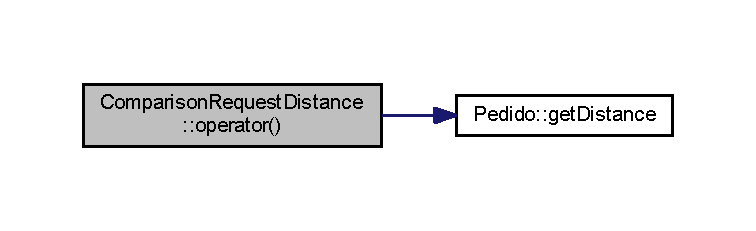
\includegraphics[width=350pt]{class_comparison_request_distance_a8df25b4ebe4b2593e35d9ae8adba5f02_cgraph}
\end{center}
\end{figure}


The documentation for this class was generated from the following file\+:\begin{DoxyCompactItemize}
\item 
\hyperlink{_utils_8h}{Utils.\+h}\end{DoxyCompactItemize}

\hypertarget{class_comparison_request_size}{}\section{Comparison\+Request\+Size Class Reference}
\label{class_comparison_request_size}\index{Comparison\+Request\+Size@{Comparison\+Request\+Size}}


{\ttfamily \#include $<$Utils.\+h$>$}

\subsection*{Public Member Functions}
\begin{DoxyCompactItemize}
\item 
bool \hyperlink{class_comparison_request_size_ac0c648f46f908edacdfc0b95ce4da888}{operator()} (\hyperlink{class_pedido}{Pedido} $\ast$a, \hyperlink{class_pedido}{Pedido} $\ast$b)
\end{DoxyCompactItemize}


\subsection{Member Function Documentation}
\mbox{\Hypertarget{class_comparison_request_size_ac0c648f46f908edacdfc0b95ce4da888}\label{class_comparison_request_size_ac0c648f46f908edacdfc0b95ce4da888}} 
\index{Comparison\+Request\+Size@{Comparison\+Request\+Size}!operator()@{operator()}}
\index{operator()@{operator()}!Comparison\+Request\+Size@{Comparison\+Request\+Size}}
\subsubsection{\texorpdfstring{operator()()}{operator()()}}
{\footnotesize\ttfamily bool Comparison\+Request\+Size\+::operator() (\begin{DoxyParamCaption}\item[{\hyperlink{class_pedido}{Pedido} $\ast$}]{a,  }\item[{\hyperlink{class_pedido}{Pedido} $\ast$}]{b }\end{DoxyParamCaption})\hspace{0.3cm}{\ttfamily [inline]}}

Operador utilizado para a ordena��o da fila de prioridade \textquotesingle{}pedidos\textquotesingle{} da classe \hyperlink{class_supermercado}{Supermercado}, de modo a que o pedido de menor tamanho esteja � cabe�a da fila. Here is the call graph for this function\+:
\nopagebreak
\begin{figure}[H]
\begin{center}
\leavevmode
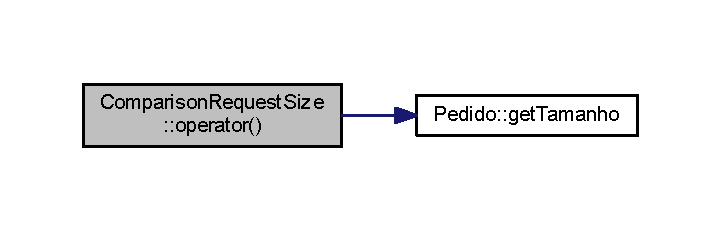
\includegraphics[width=346pt]{class_comparison_request_size_ac0c648f46f908edacdfc0b95ce4da888_cgraph}
\end{center}
\end{figure}


The documentation for this class was generated from the following file\+:\begin{DoxyCompactItemize}
\item 
\hyperlink{_utils_8h}{Utils.\+h}\end{DoxyCompactItemize}

\hypertarget{class_comparison_street_similarity}{}\section{Comparison\+Street\+Similarity Class Reference}
\label{class_comparison_street_similarity}\index{Comparison\+Street\+Similarity@{Comparison\+Street\+Similarity}}


{\ttfamily \#include $<$Supermarket\+Manager.\+h$>$}

\subsection*{Public Member Functions}
\begin{DoxyCompactItemize}
\item 
bool \hyperlink{class_comparison_street_similarity_a6f94e67250db423dcac1d1070facc60c}{operator()} (pair$<$ \hyperlink{class_edge}{Edge}$<$ \hyperlink{class_node_object}{Node\+Object} $\ast$$>$ $\ast$, int $>$ a, pair$<$ \hyperlink{class_edge}{Edge}$<$ \hyperlink{class_node_object}{Node\+Object} $\ast$$>$ $\ast$, int $>$ b)
\end{DoxyCompactItemize}


\subsection{Member Function Documentation}
\mbox{\Hypertarget{class_comparison_street_similarity_a6f94e67250db423dcac1d1070facc60c}\label{class_comparison_street_similarity_a6f94e67250db423dcac1d1070facc60c}} 
\index{Comparison\+Street\+Similarity@{Comparison\+Street\+Similarity}!operator()@{operator()}}
\index{operator()@{operator()}!Comparison\+Street\+Similarity@{Comparison\+Street\+Similarity}}
\subsubsection{\texorpdfstring{operator()()}{operator()()}}
{\footnotesize\ttfamily bool Comparison\+Street\+Similarity\+::operator() (\begin{DoxyParamCaption}\item[{pair$<$ \hyperlink{class_edge}{Edge}$<$ \hyperlink{class_node_object}{Node\+Object} $\ast$$>$ $\ast$, int $>$}]{a,  }\item[{pair$<$ \hyperlink{class_edge}{Edge}$<$ \hyperlink{class_node_object}{Node\+Object} $\ast$$>$ $\ast$, int $>$}]{b }\end{DoxyParamCaption})\hspace{0.3cm}{\ttfamily [inline]}}

Operador utilizado para a ordenacao da fila de prioridade ruas da funcao approximate\+Search\+Street, de modo a que a rua de maior similaridade esteja na cabeca da fila. 

The documentation for this class was generated from the following file\+:\begin{DoxyCompactItemize}
\item 
\hyperlink{_supermarket_manager_8h}{Supermarket\+Manager.\+h}\end{DoxyCompactItemize}

\hypertarget{class_edge}{}\section{Edge$<$ T $>$ Class Template Reference}
\label{class_edge}\index{Edge$<$ T $>$@{Edge$<$ T $>$}}


{\ttfamily \#include $<$Graph.\+h$>$}

\subsection*{Public Member Functions}
\begin{DoxyCompactItemize}
\item 
\hyperlink{class_edge_aba1f7e4e068577ca4687da274ecbb5f9}{Edge} (\hyperlink{class_vertex}{Vertex}$<$ T $>$ $\ast$d, \hyperlink{class_vertex}{Vertex}$<$ T $>$ $\ast$s, double w, string r, string di)
\item 
\hyperlink{class_vertex}{Vertex}$<$ T $>$ $\ast$ \hyperlink{class_edge_aaac5b053bdaa88b1da416e734487eb25}{get\+Dest} ()
\item 
\hyperlink{class_vertex}{Vertex}$<$ T $>$ $\ast$ \hyperlink{class_edge_a2645a9ac350e79626dc5472714b3b3b1}{get\+Src} ()
\item 
string \hyperlink{class_edge_accb828015f1926387735bc967b236bc0}{get\+Rua} ()
\item 
string \hyperlink{class_edge_a03d90697f0dd989971c4a6253cd7fa92}{get\+Distrito} ()
\end{DoxyCompactItemize}
\subsection*{Private Attributes}
\begin{DoxyCompactItemize}
\item 
\hyperlink{class_vertex}{Vertex}$<$ T $>$ $\ast$ \hyperlink{class_edge_ae4d65678b91bd9d814af4720ad87cd0c}{dest}
\item 
double \hyperlink{class_edge_af188b57b604f0d65e2da48733bd76426}{weight}
\item 
string \hyperlink{class_edge_abbe53eb540c289810569a5d67691317d}{rua}
\item 
string \hyperlink{class_edge_a5853093c36a4a3f483ce705d99f87f67}{distrito}
\item 
\hyperlink{class_vertex}{Vertex}$<$ T $>$ $\ast$ \hyperlink{class_edge_ac19036953f77507f329af34355aed4db}{src}
\end{DoxyCompactItemize}
\subsection*{Friends}
\begin{DoxyCompactItemize}
\item 
class \hyperlink{class_edge_aefa9b76cd57411c5354e5620dc2d84dd}{Graph$<$ T $>$}
\item 
class \hyperlink{class_edge_a2e120a12dec663fa334633b4f26cbed8}{Vertex$<$ T $>$}
\end{DoxyCompactItemize}


\subsection{Constructor \& Destructor Documentation}
\mbox{\Hypertarget{class_edge_aba1f7e4e068577ca4687da274ecbb5f9}\label{class_edge_aba1f7e4e068577ca4687da274ecbb5f9}} 
\index{Edge@{Edge}!Edge@{Edge}}
\index{Edge@{Edge}!Edge@{Edge}}
\subsubsection{\texorpdfstring{Edge()}{Edge()}}
{\footnotesize\ttfamily template$<$class T $>$ \\
\hyperlink{class_edge}{Edge}$<$ T $>$\+::\hyperlink{class_edge}{Edge} (\begin{DoxyParamCaption}\item[{\hyperlink{class_vertex}{Vertex}$<$ T $>$ $\ast$}]{d,  }\item[{\hyperlink{class_vertex}{Vertex}$<$ T $>$ $\ast$}]{s,  }\item[{double}]{w,  }\item[{string}]{r,  }\item[{string}]{di }\end{DoxyParamCaption})}



\subsection{Member Function Documentation}
\mbox{\Hypertarget{class_edge_aaac5b053bdaa88b1da416e734487eb25}\label{class_edge_aaac5b053bdaa88b1da416e734487eb25}} 
\index{Edge@{Edge}!get\+Dest@{get\+Dest}}
\index{get\+Dest@{get\+Dest}!Edge@{Edge}}
\subsubsection{\texorpdfstring{get\+Dest()}{getDest()}}
{\footnotesize\ttfamily template$<$class T$>$ \\
\hyperlink{class_vertex}{Vertex}$<$T$>$$\ast$ \hyperlink{class_edge}{Edge}$<$ T $>$\+::get\+Dest (\begin{DoxyParamCaption}{ }\end{DoxyParamCaption})\hspace{0.3cm}{\ttfamily [inline]}}

Here is the caller graph for this function\+:
\nopagebreak
\begin{figure}[H]
\begin{center}
\leavevmode
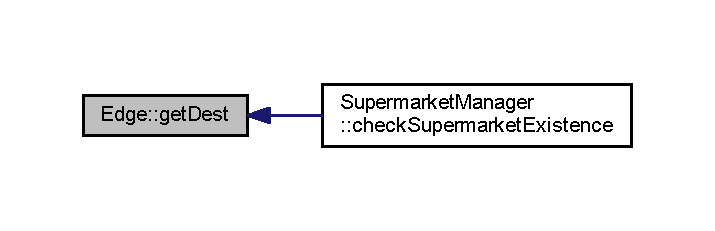
\includegraphics[width=343pt]{class_edge_aaac5b053bdaa88b1da416e734487eb25_icgraph}
\end{center}
\end{figure}
\mbox{\Hypertarget{class_edge_a03d90697f0dd989971c4a6253cd7fa92}\label{class_edge_a03d90697f0dd989971c4a6253cd7fa92}} 
\index{Edge@{Edge}!get\+Distrito@{get\+Distrito}}
\index{get\+Distrito@{get\+Distrito}!Edge@{Edge}}
\subsubsection{\texorpdfstring{get\+Distrito()}{getDistrito()}}
{\footnotesize\ttfamily template$<$class T$>$ \\
string \hyperlink{class_edge}{Edge}$<$ T $>$\+::get\+Distrito (\begin{DoxyParamCaption}{ }\end{DoxyParamCaption})\hspace{0.3cm}{\ttfamily [inline]}}

\mbox{\Hypertarget{class_edge_accb828015f1926387735bc967b236bc0}\label{class_edge_accb828015f1926387735bc967b236bc0}} 
\index{Edge@{Edge}!get\+Rua@{get\+Rua}}
\index{get\+Rua@{get\+Rua}!Edge@{Edge}}
\subsubsection{\texorpdfstring{get\+Rua()}{getRua()}}
{\footnotesize\ttfamily template$<$class T$>$ \\
string \hyperlink{class_edge}{Edge}$<$ T $>$\+::get\+Rua (\begin{DoxyParamCaption}{ }\end{DoxyParamCaption})\hspace{0.3cm}{\ttfamily [inline]}}

\mbox{\Hypertarget{class_edge_a2645a9ac350e79626dc5472714b3b3b1}\label{class_edge_a2645a9ac350e79626dc5472714b3b3b1}} 
\index{Edge@{Edge}!get\+Src@{get\+Src}}
\index{get\+Src@{get\+Src}!Edge@{Edge}}
\subsubsection{\texorpdfstring{get\+Src()}{getSrc()}}
{\footnotesize\ttfamily template$<$class T$>$ \\
\hyperlink{class_vertex}{Vertex}$<$T$>$$\ast$ \hyperlink{class_edge}{Edge}$<$ T $>$\+::get\+Src (\begin{DoxyParamCaption}{ }\end{DoxyParamCaption})\hspace{0.3cm}{\ttfamily [inline]}}

Here is the caller graph for this function\+:
\nopagebreak
\begin{figure}[H]
\begin{center}
\leavevmode
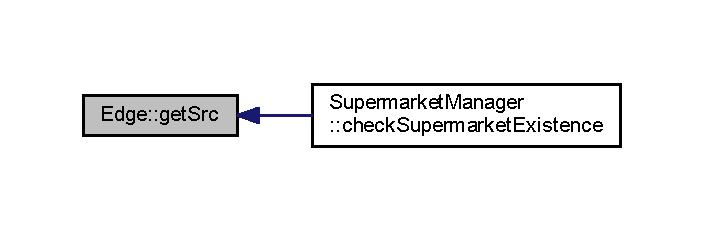
\includegraphics[width=338pt]{class_edge_a2645a9ac350e79626dc5472714b3b3b1_icgraph}
\end{center}
\end{figure}


\subsection{Friends And Related Function Documentation}
\mbox{\Hypertarget{class_edge_aefa9b76cd57411c5354e5620dc2d84dd}\label{class_edge_aefa9b76cd57411c5354e5620dc2d84dd}} 
\index{Edge@{Edge}!Graph$<$ T $>$@{Graph$<$ T $>$}}
\index{Graph$<$ T $>$@{Graph$<$ T $>$}!Edge@{Edge}}
\subsubsection{\texorpdfstring{Graph$<$ T $>$}{Graph< T >}}
{\footnotesize\ttfamily template$<$class T$>$ \\
friend class \hyperlink{class_graph}{Graph}$<$ T $>$\hspace{0.3cm}{\ttfamily [friend]}}

\mbox{\Hypertarget{class_edge_a2e120a12dec663fa334633b4f26cbed8}\label{class_edge_a2e120a12dec663fa334633b4f26cbed8}} 
\index{Edge@{Edge}!Vertex$<$ T $>$@{Vertex$<$ T $>$}}
\index{Vertex$<$ T $>$@{Vertex$<$ T $>$}!Edge@{Edge}}
\subsubsection{\texorpdfstring{Vertex$<$ T $>$}{Vertex< T >}}
{\footnotesize\ttfamily template$<$class T$>$ \\
friend class \hyperlink{class_vertex}{Vertex}$<$ T $>$\hspace{0.3cm}{\ttfamily [friend]}}



\subsection{Member Data Documentation}
\mbox{\Hypertarget{class_edge_ae4d65678b91bd9d814af4720ad87cd0c}\label{class_edge_ae4d65678b91bd9d814af4720ad87cd0c}} 
\index{Edge@{Edge}!dest@{dest}}
\index{dest@{dest}!Edge@{Edge}}
\subsubsection{\texorpdfstring{dest}{dest}}
{\footnotesize\ttfamily template$<$class T$>$ \\
\hyperlink{class_vertex}{Vertex}$<$T$>$$\ast$ \hyperlink{class_edge}{Edge}$<$ T $>$\+::dest\hspace{0.3cm}{\ttfamily [private]}}

\mbox{\Hypertarget{class_edge_a5853093c36a4a3f483ce705d99f87f67}\label{class_edge_a5853093c36a4a3f483ce705d99f87f67}} 
\index{Edge@{Edge}!distrito@{distrito}}
\index{distrito@{distrito}!Edge@{Edge}}
\subsubsection{\texorpdfstring{distrito}{distrito}}
{\footnotesize\ttfamily template$<$class T$>$ \\
string \hyperlink{class_edge}{Edge}$<$ T $>$\+::distrito\hspace{0.3cm}{\ttfamily [private]}}

\mbox{\Hypertarget{class_edge_abbe53eb540c289810569a5d67691317d}\label{class_edge_abbe53eb540c289810569a5d67691317d}} 
\index{Edge@{Edge}!rua@{rua}}
\index{rua@{rua}!Edge@{Edge}}
\subsubsection{\texorpdfstring{rua}{rua}}
{\footnotesize\ttfamily template$<$class T$>$ \\
string \hyperlink{class_edge}{Edge}$<$ T $>$\+::rua\hspace{0.3cm}{\ttfamily [private]}}

\mbox{\Hypertarget{class_edge_ac19036953f77507f329af34355aed4db}\label{class_edge_ac19036953f77507f329af34355aed4db}} 
\index{Edge@{Edge}!src@{src}}
\index{src@{src}!Edge@{Edge}}
\subsubsection{\texorpdfstring{src}{src}}
{\footnotesize\ttfamily template$<$class T$>$ \\
\hyperlink{class_vertex}{Vertex}$<$T$>$$\ast$ \hyperlink{class_edge}{Edge}$<$ T $>$\+::src\hspace{0.3cm}{\ttfamily [private]}}

\mbox{\Hypertarget{class_edge_af188b57b604f0d65e2da48733bd76426}\label{class_edge_af188b57b604f0d65e2da48733bd76426}} 
\index{Edge@{Edge}!weight@{weight}}
\index{weight@{weight}!Edge@{Edge}}
\subsubsection{\texorpdfstring{weight}{weight}}
{\footnotesize\ttfamily template$<$class T$>$ \\
double \hyperlink{class_edge}{Edge}$<$ T $>$\+::weight\hspace{0.3cm}{\ttfamily [private]}}



The documentation for this class was generated from the following file\+:\begin{DoxyCompactItemize}
\item 
\hyperlink{_graph_8h}{Graph.\+h}\end{DoxyCompactItemize}

\hypertarget{class_graph}{}\section{Graph$<$ T $>$ Class Template Reference}
\label{class_graph}\index{Graph$<$ T $>$@{Graph$<$ T $>$}}


{\ttfamily \#include $<$Graph.\+h$>$}

\subsection*{Public Member Functions}
\begin{DoxyCompactItemize}
\item 
bool \hyperlink{class_graph_a00be284ea2be3b3d0f0d2e493b70245b}{add\+Vertex} (const T \&in)
\item 
bool \hyperlink{class_graph_ad7d2d102d0b5e91345d69766e1adcd19}{add\+Edge} (const T \&sourc, const T \&dest, double w, string r, string d)
\item 
bool \hyperlink{class_graph_af9c903104ad69a7782979fa9caedf163}{remove\+Vertex} (const T \&in)
\item 
bool \hyperlink{class_graph_a1106092a37366486cf55576f9ec01692}{remove\+Edge} (const T \&sourc, const T \&dest)
\item 
vector$<$ T $>$ \hyperlink{class_graph_a911798b1a89f8c4ae90ba3eee849cff8}{dfs} () const
\item 
vector$<$ T $>$ \hyperlink{class_graph_a56a5ea2c3aa7c0bd3849849be404a631}{bfs} (\hyperlink{class_vertex}{Vertex}$<$ T $>$ $\ast$v) const
\item 
int \hyperlink{class_graph_a675559f8cddfe43bc416023ad9f28cfa}{max\+New\+Children} (\hyperlink{class_vertex}{Vertex}$<$ T $>$ $\ast$v, T \&inf) const
\item 
vector$<$ \hyperlink{class_vertex}{Vertex}$<$ T $>$ $\ast$$>$ \hyperlink{class_graph_a135e8f915af85904abca9eafaa4f13ce}{get\+Vertex\+Set} () const
\item 
int \hyperlink{class_graph_a0853eac15cdf0f06d63f4b8a7820ec71}{get\+Num\+Vertex} () const
\item 
\hyperlink{class_vertex}{Vertex}$<$ T $>$ $\ast$ \hyperlink{class_graph_a67453d232f04e85c642b51554df1bc6a}{get\+Vertex} (const T \&v) const
\item 
vector$<$ \hyperlink{class_edge}{Edge}$<$ T $>$ $>$ \hyperlink{class_graph_a92ccadde8c981252b715147a33b9dcb1}{get\+Edges} ()
\item 
void \hyperlink{class_graph_af34eb86d804272e6e3e221a9ed688c53}{reset\+Indegrees} ()
\item 
vector$<$ \hyperlink{class_vertex}{Vertex}$<$ T $>$ $\ast$ $>$ \hyperlink{class_graph_a947115150a94f88ac9aedbcec59dd07e}{get\+Sources} () const
\item 
int \hyperlink{class_graph_a694dff81073c38b669057f0c6bd4cbb1}{get\+Num\+Cycles} ()
\item 
bool \hyperlink{class_graph_ab49d07c2bd6b8b30d5ae82bc558b821a}{is\+D\+AG} ()
\item 
vector$<$ T $>$ \hyperlink{class_graph_a2e75512c089c3916dda9cf61e1185d9d}{topological\+Order} ()
\item 
vector$<$ T $>$ \hyperlink{class_graph_ab4054ca572c10669dd3e05d6d41c116c}{get\+Path} (const T \&origin, const T \&dest)
\item 
void \hyperlink{class_graph_ae5264597aacaf4f45819e96a6d6c89aa}{unweighted\+Shortest\+Path} (const T \&v)
\item 
void \hyperlink{class_graph_ad0319019c0883094c0d09841e88f2179}{dijkstra} (\hyperlink{class_vertex}{Vertex}$<$ T $>$ $\ast$origin)
\item 
\hyperlink{class_graph}{Graph}$<$ T $>$ \hyperlink{class_graph_a153095b4dd52f90027f8a7ac3fc5d2ab}{get\+Transpose} ()
\item 
void \hyperlink{class_graph_a56fefa2bdd0f7d66eec0ef51c961846a}{dfs\+Print} (\hyperlink{class_vertex}{Vertex}$<$ T $>$ $\ast$v) const
\end{DoxyCompactItemize}
\subsection*{Private Member Functions}
\begin{DoxyCompactItemize}
\item 
void \hyperlink{class_graph_abf3a280505ad7abd0ff83f45eb807c41}{dfs} (\hyperlink{class_vertex}{Vertex}$<$ T $>$ $\ast$v, vector$<$ T $>$ \&res) const
\item 
void \hyperlink{class_graph_a167172d4ecb3f4998caaaf370724b536}{dfs\+Visit} (\hyperlink{class_vertex}{Vertex}$<$ T $>$ $\ast$v)
\item 
void \hyperlink{class_graph_a4d5abd78dd24ea71dbf50e1b0284d4b3}{dfs\+Visit} ()
\item 
void \hyperlink{class_graph_ac08257ce8a96a8b4e44f1818e5eb8cf9}{get\+Path\+To} (\hyperlink{class_vertex}{Vertex}$<$ T $>$ $\ast$origin, list$<$ T $>$ \&res)
\end{DoxyCompactItemize}
\subsection*{Private Attributes}
\begin{DoxyCompactItemize}
\item 
vector$<$ \hyperlink{class_vertex}{Vertex}$<$ T $>$ $\ast$ $>$ \hyperlink{class_graph_a73d4e735fc0a7c83c9c689a2b53fa623}{vertex\+Set}
\item 
vector$<$ \hyperlink{class_edge}{Edge}$<$ T $>$ $>$ \hyperlink{class_graph_a9cb12007e85c47011141b52cf565e0ed}{edge\+Set}
\item 
int \hyperlink{class_graph_ad5cc402f1b24d30ae12ffc2622ffbd5f}{num\+Cycles}
\end{DoxyCompactItemize}


\subsection{Member Function Documentation}
\mbox{\Hypertarget{class_graph_ad7d2d102d0b5e91345d69766e1adcd19}\label{class_graph_ad7d2d102d0b5e91345d69766e1adcd19}} 
\index{Graph@{Graph}!add\+Edge@{add\+Edge}}
\index{add\+Edge@{add\+Edge}!Graph@{Graph}}
\subsubsection{\texorpdfstring{add\+Edge()}{addEdge()}}
{\footnotesize\ttfamily template$<$class T$>$ \\
bool \hyperlink{class_graph}{Graph}$<$ T $>$\+::add\+Edge (\begin{DoxyParamCaption}\item[{const T \&}]{sourc,  }\item[{const T \&}]{dest,  }\item[{double}]{w,  }\item[{string}]{r,  }\item[{string}]{d }\end{DoxyParamCaption})}

Here is the caller graph for this function\+:
\nopagebreak
\begin{figure}[H]
\begin{center}
\leavevmode
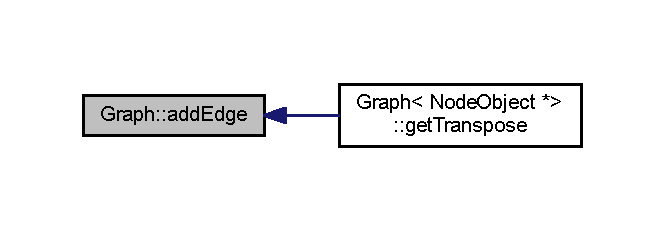
\includegraphics[width=319pt]{class_graph_ad7d2d102d0b5e91345d69766e1adcd19_icgraph}
\end{center}
\end{figure}
\mbox{\Hypertarget{class_graph_a00be284ea2be3b3d0f0d2e493b70245b}\label{class_graph_a00be284ea2be3b3d0f0d2e493b70245b}} 
\index{Graph@{Graph}!add\+Vertex@{add\+Vertex}}
\index{add\+Vertex@{add\+Vertex}!Graph@{Graph}}
\subsubsection{\texorpdfstring{add\+Vertex()}{addVertex()}}
{\footnotesize\ttfamily template$<$class T$>$ \\
bool \hyperlink{class_graph}{Graph}$<$ T $>$\+::add\+Vertex (\begin{DoxyParamCaption}\item[{const T \&}]{in }\end{DoxyParamCaption})}

Here is the caller graph for this function\+:
\nopagebreak
\begin{figure}[H]
\begin{center}
\leavevmode
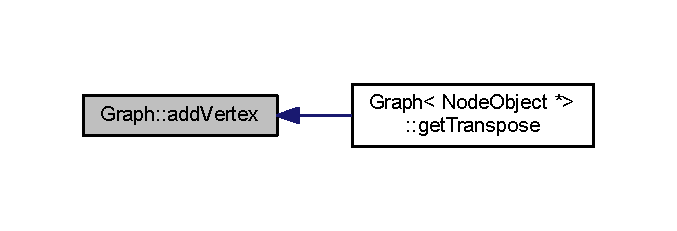
\includegraphics[width=325pt]{class_graph_a00be284ea2be3b3d0f0d2e493b70245b_icgraph}
\end{center}
\end{figure}
\mbox{\Hypertarget{class_graph_a56a5ea2c3aa7c0bd3849849be404a631}\label{class_graph_a56a5ea2c3aa7c0bd3849849be404a631}} 
\index{Graph@{Graph}!bfs@{bfs}}
\index{bfs@{bfs}!Graph@{Graph}}
\subsubsection{\texorpdfstring{bfs()}{bfs()}}
{\footnotesize\ttfamily template$<$class T$>$ \\
vector$<$ T $>$ \hyperlink{class_graph}{Graph}$<$ T $>$\+::bfs (\begin{DoxyParamCaption}\item[{\hyperlink{class_vertex}{Vertex}$<$ T $>$ $\ast$}]{v }\end{DoxyParamCaption}) const}

\mbox{\Hypertarget{class_graph_abf3a280505ad7abd0ff83f45eb807c41}\label{class_graph_abf3a280505ad7abd0ff83f45eb807c41}} 
\index{Graph@{Graph}!dfs@{dfs}}
\index{dfs@{dfs}!Graph@{Graph}}
\subsubsection{\texorpdfstring{dfs()}{dfs()}\hspace{0.1cm}{\footnotesize\ttfamily [1/2]}}
{\footnotesize\ttfamily template$<$class T$>$ \\
void \hyperlink{class_graph}{Graph}$<$ T $>$\+::dfs (\begin{DoxyParamCaption}\item[{\hyperlink{class_vertex}{Vertex}$<$ T $>$ $\ast$}]{v,  }\item[{vector$<$ T $>$ \&}]{res }\end{DoxyParamCaption}) const\hspace{0.3cm}{\ttfamily [private]}}

\mbox{\Hypertarget{class_graph_a911798b1a89f8c4ae90ba3eee849cff8}\label{class_graph_a911798b1a89f8c4ae90ba3eee849cff8}} 
\index{Graph@{Graph}!dfs@{dfs}}
\index{dfs@{dfs}!Graph@{Graph}}
\subsubsection{\texorpdfstring{dfs()}{dfs()}\hspace{0.1cm}{\footnotesize\ttfamily [2/2]}}
{\footnotesize\ttfamily template$<$class T$>$ \\
vector$<$ T $>$ \hyperlink{class_graph}{Graph}$<$ T $>$\+::dfs (\begin{DoxyParamCaption}{ }\end{DoxyParamCaption}) const}

\mbox{\Hypertarget{class_graph_a56fefa2bdd0f7d66eec0ef51c961846a}\label{class_graph_a56fefa2bdd0f7d66eec0ef51c961846a}} 
\index{Graph@{Graph}!dfs\+Print@{dfs\+Print}}
\index{dfs\+Print@{dfs\+Print}!Graph@{Graph}}
\subsubsection{\texorpdfstring{dfs\+Print()}{dfsPrint()}}
{\footnotesize\ttfamily template$<$class T$>$ \\
void \hyperlink{class_graph}{Graph}$<$ T $>$\+::dfs\+Print (\begin{DoxyParamCaption}\item[{\hyperlink{class_vertex}{Vertex}$<$ T $>$ $\ast$}]{v }\end{DoxyParamCaption}) const}

Imprime o conteudo dos vertices do grafo pela ordem em que os visita em profundidade.


\begin{DoxyParams}{Parameters}
{\em v} & apontador para o vertice de inicio \\
\hline
\end{DoxyParams}
Here is the caller graph for this function\+:
\nopagebreak
\begin{figure}[H]
\begin{center}
\leavevmode
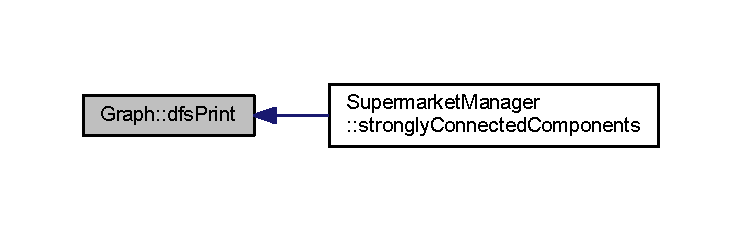
\includegraphics[width=350pt]{class_graph_a56fefa2bdd0f7d66eec0ef51c961846a_icgraph}
\end{center}
\end{figure}
\mbox{\Hypertarget{class_graph_a167172d4ecb3f4998caaaf370724b536}\label{class_graph_a167172d4ecb3f4998caaaf370724b536}} 
\index{Graph@{Graph}!dfs\+Visit@{dfs\+Visit}}
\index{dfs\+Visit@{dfs\+Visit}!Graph@{Graph}}
\subsubsection{\texorpdfstring{dfs\+Visit()}{dfsVisit()}\hspace{0.1cm}{\footnotesize\ttfamily [1/2]}}
{\footnotesize\ttfamily template$<$class T$>$ \\
void \hyperlink{class_graph}{Graph}$<$ T $>$\+::dfs\+Visit (\begin{DoxyParamCaption}\item[{\hyperlink{class_vertex}{Vertex}$<$ T $>$ $\ast$}]{v }\end{DoxyParamCaption})\hspace{0.3cm}{\ttfamily [private]}}

\mbox{\Hypertarget{class_graph_a4d5abd78dd24ea71dbf50e1b0284d4b3}\label{class_graph_a4d5abd78dd24ea71dbf50e1b0284d4b3}} 
\index{Graph@{Graph}!dfs\+Visit@{dfs\+Visit}}
\index{dfs\+Visit@{dfs\+Visit}!Graph@{Graph}}
\subsubsection{\texorpdfstring{dfs\+Visit()}{dfsVisit()}\hspace{0.1cm}{\footnotesize\ttfamily [2/2]}}
{\footnotesize\ttfamily template$<$class T$>$ \\
void \hyperlink{class_graph}{Graph}$<$ T $>$\+::dfs\+Visit (\begin{DoxyParamCaption}{ }\end{DoxyParamCaption})\hspace{0.3cm}{\ttfamily [private]}}

\mbox{\Hypertarget{class_graph_ad0319019c0883094c0d09841e88f2179}\label{class_graph_ad0319019c0883094c0d09841e88f2179}} 
\index{Graph@{Graph}!dijkstra@{dijkstra}}
\index{dijkstra@{dijkstra}!Graph@{Graph}}
\subsubsection{\texorpdfstring{dijkstra()}{dijkstra()}}
{\footnotesize\ttfamily template$<$class T$>$ \\
void \hyperlink{class_graph}{Graph}$<$ T $>$\+::dijkstra (\begin{DoxyParamCaption}\item[{\hyperlink{class_vertex}{Vertex}$<$ T $>$ $\ast$}]{origin }\end{DoxyParamCaption})}

Here is the caller graph for this function\+:
\nopagebreak
\begin{figure}[H]
\begin{center}
\leavevmode
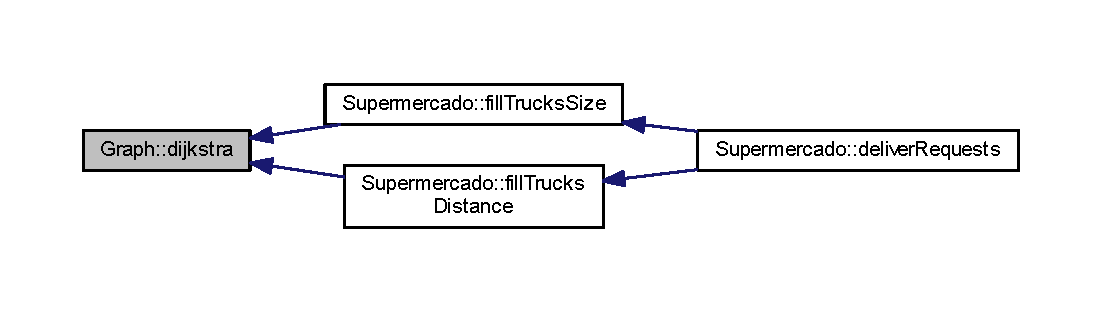
\includegraphics[width=350pt]{class_graph_ad0319019c0883094c0d09841e88f2179_icgraph}
\end{center}
\end{figure}
\mbox{\Hypertarget{class_graph_a92ccadde8c981252b715147a33b9dcb1}\label{class_graph_a92ccadde8c981252b715147a33b9dcb1}} 
\index{Graph@{Graph}!get\+Edges@{get\+Edges}}
\index{get\+Edges@{get\+Edges}!Graph@{Graph}}
\subsubsection{\texorpdfstring{get\+Edges()}{getEdges()}}
{\footnotesize\ttfamily template$<$class T$>$ \\
vector$<$\hyperlink{class_edge}{Edge}$<$T$>$ $>$ \hyperlink{class_graph}{Graph}$<$ T $>$\+::get\+Edges (\begin{DoxyParamCaption}{ }\end{DoxyParamCaption})\hspace{0.3cm}{\ttfamily [inline]}}

\mbox{\Hypertarget{class_graph_a694dff81073c38b669057f0c6bd4cbb1}\label{class_graph_a694dff81073c38b669057f0c6bd4cbb1}} 
\index{Graph@{Graph}!get\+Num\+Cycles@{get\+Num\+Cycles}}
\index{get\+Num\+Cycles@{get\+Num\+Cycles}!Graph@{Graph}}
\subsubsection{\texorpdfstring{get\+Num\+Cycles()}{getNumCycles()}}
{\footnotesize\ttfamily template$<$class T $>$ \\
int \hyperlink{class_graph}{Graph}$<$ T $>$\+::get\+Num\+Cycles (\begin{DoxyParamCaption}{ }\end{DoxyParamCaption})}

\mbox{\Hypertarget{class_graph_a0853eac15cdf0f06d63f4b8a7820ec71}\label{class_graph_a0853eac15cdf0f06d63f4b8a7820ec71}} 
\index{Graph@{Graph}!get\+Num\+Vertex@{get\+Num\+Vertex}}
\index{get\+Num\+Vertex@{get\+Num\+Vertex}!Graph@{Graph}}
\subsubsection{\texorpdfstring{get\+Num\+Vertex()}{getNumVertex()}}
{\footnotesize\ttfamily template$<$class T $>$ \\
int \hyperlink{class_graph}{Graph}$<$ T $>$\+::get\+Num\+Vertex (\begin{DoxyParamCaption}{ }\end{DoxyParamCaption}) const}

\mbox{\Hypertarget{class_graph_ab4054ca572c10669dd3e05d6d41c116c}\label{class_graph_ab4054ca572c10669dd3e05d6d41c116c}} 
\index{Graph@{Graph}!get\+Path@{get\+Path}}
\index{get\+Path@{get\+Path}!Graph@{Graph}}
\subsubsection{\texorpdfstring{get\+Path()}{getPath()}}
{\footnotesize\ttfamily template$<$class T$>$ \\
vector$<$ T $>$ \hyperlink{class_graph}{Graph}$<$ T $>$\+::get\+Path (\begin{DoxyParamCaption}\item[{const T \&}]{origin,  }\item[{const T \&}]{dest }\end{DoxyParamCaption})}

\mbox{\Hypertarget{class_graph_ac08257ce8a96a8b4e44f1818e5eb8cf9}\label{class_graph_ac08257ce8a96a8b4e44f1818e5eb8cf9}} 
\index{Graph@{Graph}!get\+Path\+To@{get\+Path\+To}}
\index{get\+Path\+To@{get\+Path\+To}!Graph@{Graph}}
\subsubsection{\texorpdfstring{get\+Path\+To()}{getPathTo()}}
{\footnotesize\ttfamily template$<$class T$>$ \\
void \hyperlink{class_graph}{Graph}$<$ T $>$\+::get\+Path\+To (\begin{DoxyParamCaption}\item[{\hyperlink{class_vertex}{Vertex}$<$ T $>$ $\ast$}]{origin,  }\item[{list$<$ T $>$ \&}]{res }\end{DoxyParamCaption})\hspace{0.3cm}{\ttfamily [private]}}

\mbox{\Hypertarget{class_graph_a947115150a94f88ac9aedbcec59dd07e}\label{class_graph_a947115150a94f88ac9aedbcec59dd07e}} 
\index{Graph@{Graph}!get\+Sources@{get\+Sources}}
\index{get\+Sources@{get\+Sources}!Graph@{Graph}}
\subsubsection{\texorpdfstring{get\+Sources()}{getSources()}}
{\footnotesize\ttfamily template$<$class T $>$ \\
vector$<$ \hyperlink{class_vertex}{Vertex}$<$ T $>$ $\ast$ $>$ \hyperlink{class_graph}{Graph}$<$ T $>$\+::get\+Sources (\begin{DoxyParamCaption}{ }\end{DoxyParamCaption}) const}

\mbox{\Hypertarget{class_graph_a153095b4dd52f90027f8a7ac3fc5d2ab}\label{class_graph_a153095b4dd52f90027f8a7ac3fc5d2ab}} 
\index{Graph@{Graph}!get\+Transpose@{get\+Transpose}}
\index{get\+Transpose@{get\+Transpose}!Graph@{Graph}}
\subsubsection{\texorpdfstring{get\+Transpose()}{getTranspose()}}
{\footnotesize\ttfamily template$<$class T $>$ \\
\hyperlink{class_graph}{Graph}$<$ T $>$ \hyperlink{class_graph}{Graph}$<$ T $>$\+::get\+Transpose (\begin{DoxyParamCaption}{ }\end{DoxyParamCaption})}

Inverte o sentido das arestas de um grafo.

\begin{DoxyReturn}{Returns}
grafo invertido 
\end{DoxyReturn}
Here is the caller graph for this function\+:
\nopagebreak
\begin{figure}[H]
\begin{center}
\leavevmode
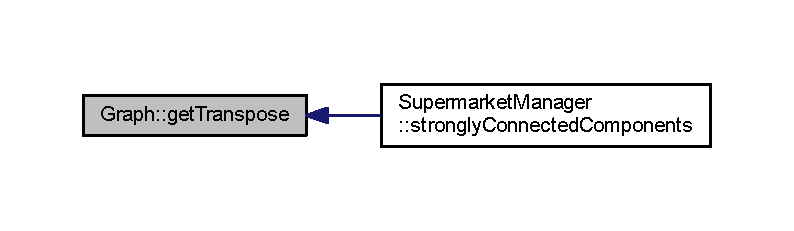
\includegraphics[width=350pt]{class_graph_a153095b4dd52f90027f8a7ac3fc5d2ab_icgraph}
\end{center}
\end{figure}
\mbox{\Hypertarget{class_graph_a67453d232f04e85c642b51554df1bc6a}\label{class_graph_a67453d232f04e85c642b51554df1bc6a}} 
\index{Graph@{Graph}!get\+Vertex@{get\+Vertex}}
\index{get\+Vertex@{get\+Vertex}!Graph@{Graph}}
\subsubsection{\texorpdfstring{get\+Vertex()}{getVertex()}}
{\footnotesize\ttfamily template$<$class T$>$ \\
\hyperlink{class_vertex}{Vertex}$<$ T $>$ $\ast$ \hyperlink{class_graph}{Graph}$<$ T $>$\+::get\+Vertex (\begin{DoxyParamCaption}\item[{const T \&}]{v }\end{DoxyParamCaption}) const}

Here is the caller graph for this function\+:
\nopagebreak
\begin{figure}[H]
\begin{center}
\leavevmode
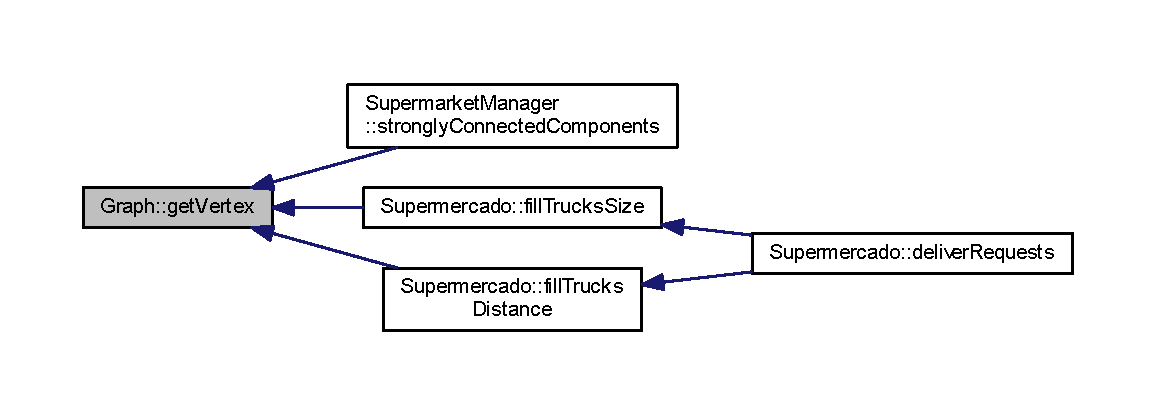
\includegraphics[width=350pt]{class_graph_a67453d232f04e85c642b51554df1bc6a_icgraph}
\end{center}
\end{figure}
\mbox{\Hypertarget{class_graph_a135e8f915af85904abca9eafaa4f13ce}\label{class_graph_a135e8f915af85904abca9eafaa4f13ce}} 
\index{Graph@{Graph}!get\+Vertex\+Set@{get\+Vertex\+Set}}
\index{get\+Vertex\+Set@{get\+Vertex\+Set}!Graph@{Graph}}
\subsubsection{\texorpdfstring{get\+Vertex\+Set()}{getVertexSet()}}
{\footnotesize\ttfamily template$<$class T $>$ \\
vector$<$ \hyperlink{class_vertex}{Vertex}$<$ T $>$ $\ast$$>$ \hyperlink{class_graph}{Graph}$<$ T $>$\+::get\+Vertex\+Set (\begin{DoxyParamCaption}{ }\end{DoxyParamCaption}) const}

Here is the caller graph for this function\+:
\nopagebreak
\begin{figure}[H]
\begin{center}
\leavevmode
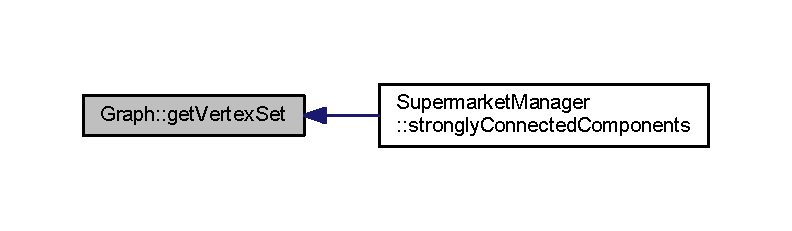
\includegraphics[width=350pt]{class_graph_a135e8f915af85904abca9eafaa4f13ce_icgraph}
\end{center}
\end{figure}
\mbox{\Hypertarget{class_graph_ab49d07c2bd6b8b30d5ae82bc558b821a}\label{class_graph_ab49d07c2bd6b8b30d5ae82bc558b821a}} 
\index{Graph@{Graph}!is\+D\+AG@{is\+D\+AG}}
\index{is\+D\+AG@{is\+D\+AG}!Graph@{Graph}}
\subsubsection{\texorpdfstring{is\+D\+A\+G()}{isDAG()}}
{\footnotesize\ttfamily template$<$class T $>$ \\
bool \hyperlink{class_graph}{Graph}$<$ T $>$\+::is\+D\+AG (\begin{DoxyParamCaption}{ }\end{DoxyParamCaption})}

\mbox{\Hypertarget{class_graph_a675559f8cddfe43bc416023ad9f28cfa}\label{class_graph_a675559f8cddfe43bc416023ad9f28cfa}} 
\index{Graph@{Graph}!max\+New\+Children@{max\+New\+Children}}
\index{max\+New\+Children@{max\+New\+Children}!Graph@{Graph}}
\subsubsection{\texorpdfstring{max\+New\+Children()}{maxNewChildren()}}
{\footnotesize\ttfamily template$<$class T$>$ \\
int \hyperlink{class_graph}{Graph}$<$ T $>$\+::max\+New\+Children (\begin{DoxyParamCaption}\item[{\hyperlink{class_vertex}{Vertex}$<$ T $>$ $\ast$}]{v,  }\item[{T \&}]{inf }\end{DoxyParamCaption}) const}

\mbox{\Hypertarget{class_graph_a1106092a37366486cf55576f9ec01692}\label{class_graph_a1106092a37366486cf55576f9ec01692}} 
\index{Graph@{Graph}!remove\+Edge@{remove\+Edge}}
\index{remove\+Edge@{remove\+Edge}!Graph@{Graph}}
\subsubsection{\texorpdfstring{remove\+Edge()}{removeEdge()}}
{\footnotesize\ttfamily template$<$class T$>$ \\
bool \hyperlink{class_graph}{Graph}$<$ T $>$\+::remove\+Edge (\begin{DoxyParamCaption}\item[{const T \&}]{sourc,  }\item[{const T \&}]{dest }\end{DoxyParamCaption})}

\mbox{\Hypertarget{class_graph_af9c903104ad69a7782979fa9caedf163}\label{class_graph_af9c903104ad69a7782979fa9caedf163}} 
\index{Graph@{Graph}!remove\+Vertex@{remove\+Vertex}}
\index{remove\+Vertex@{remove\+Vertex}!Graph@{Graph}}
\subsubsection{\texorpdfstring{remove\+Vertex()}{removeVertex()}}
{\footnotesize\ttfamily template$<$class T$>$ \\
bool \hyperlink{class_graph}{Graph}$<$ T $>$\+::remove\+Vertex (\begin{DoxyParamCaption}\item[{const T \&}]{in }\end{DoxyParamCaption})}

\mbox{\Hypertarget{class_graph_af34eb86d804272e6e3e221a9ed688c53}\label{class_graph_af34eb86d804272e6e3e221a9ed688c53}} 
\index{Graph@{Graph}!reset\+Indegrees@{reset\+Indegrees}}
\index{reset\+Indegrees@{reset\+Indegrees}!Graph@{Graph}}
\subsubsection{\texorpdfstring{reset\+Indegrees()}{resetIndegrees()}}
{\footnotesize\ttfamily template$<$class T $>$ \\
void \hyperlink{class_graph}{Graph}$<$ T $>$\+::reset\+Indegrees (\begin{DoxyParamCaption}{ }\end{DoxyParamCaption})}

\mbox{\Hypertarget{class_graph_a2e75512c089c3916dda9cf61e1185d9d}\label{class_graph_a2e75512c089c3916dda9cf61e1185d9d}} 
\index{Graph@{Graph}!topological\+Order@{topological\+Order}}
\index{topological\+Order@{topological\+Order}!Graph@{Graph}}
\subsubsection{\texorpdfstring{topological\+Order()}{topologicalOrder()}}
{\footnotesize\ttfamily template$<$class T $>$ \\
vector$<$ T $>$ \hyperlink{class_graph}{Graph}$<$ T $>$\+::topological\+Order (\begin{DoxyParamCaption}{ }\end{DoxyParamCaption})}

\mbox{\Hypertarget{class_graph_ae5264597aacaf4f45819e96a6d6c89aa}\label{class_graph_ae5264597aacaf4f45819e96a6d6c89aa}} 
\index{Graph@{Graph}!unweighted\+Shortest\+Path@{unweighted\+Shortest\+Path}}
\index{unweighted\+Shortest\+Path@{unweighted\+Shortest\+Path}!Graph@{Graph}}
\subsubsection{\texorpdfstring{unweighted\+Shortest\+Path()}{unweightedShortestPath()}}
{\footnotesize\ttfamily template$<$class T$>$ \\
void \hyperlink{class_graph}{Graph}$<$ T $>$\+::unweighted\+Shortest\+Path (\begin{DoxyParamCaption}\item[{const T \&}]{v }\end{DoxyParamCaption})}



\subsection{Member Data Documentation}
\mbox{\Hypertarget{class_graph_a9cb12007e85c47011141b52cf565e0ed}\label{class_graph_a9cb12007e85c47011141b52cf565e0ed}} 
\index{Graph@{Graph}!edge\+Set@{edge\+Set}}
\index{edge\+Set@{edge\+Set}!Graph@{Graph}}
\subsubsection{\texorpdfstring{edge\+Set}{edgeSet}}
{\footnotesize\ttfamily template$<$class T$>$ \\
vector$<$\hyperlink{class_edge}{Edge}$<$T$>$ $>$ \hyperlink{class_graph}{Graph}$<$ T $>$\+::edge\+Set\hspace{0.3cm}{\ttfamily [private]}}

\mbox{\Hypertarget{class_graph_ad5cc402f1b24d30ae12ffc2622ffbd5f}\label{class_graph_ad5cc402f1b24d30ae12ffc2622ffbd5f}} 
\index{Graph@{Graph}!num\+Cycles@{num\+Cycles}}
\index{num\+Cycles@{num\+Cycles}!Graph@{Graph}}
\subsubsection{\texorpdfstring{num\+Cycles}{numCycles}}
{\footnotesize\ttfamily template$<$class T$>$ \\
int \hyperlink{class_graph}{Graph}$<$ T $>$\+::num\+Cycles\hspace{0.3cm}{\ttfamily [private]}}

\mbox{\Hypertarget{class_graph_a73d4e735fc0a7c83c9c689a2b53fa623}\label{class_graph_a73d4e735fc0a7c83c9c689a2b53fa623}} 
\index{Graph@{Graph}!vertex\+Set@{vertex\+Set}}
\index{vertex\+Set@{vertex\+Set}!Graph@{Graph}}
\subsubsection{\texorpdfstring{vertex\+Set}{vertexSet}}
{\footnotesize\ttfamily template$<$class T$>$ \\
vector$<$\hyperlink{class_vertex}{Vertex}$<$T$>$ $\ast$$>$ \hyperlink{class_graph}{Graph}$<$ T $>$\+::vertex\+Set\hspace{0.3cm}{\ttfamily [private]}}



The documentation for this class was generated from the following file\+:\begin{DoxyCompactItemize}
\item 
\hyperlink{_graph_8h}{Graph.\+h}\end{DoxyCompactItemize}

\hypertarget{class_menu}{}\section{Menu Class Reference}
\label{class_menu}\index{Menu@{Menu}}


{\ttfamily \#include $<$Menu.\+h$>$}



Collaboration diagram for Menu\+:
\nopagebreak
\begin{figure}[H]
\begin{center}
\leavevmode
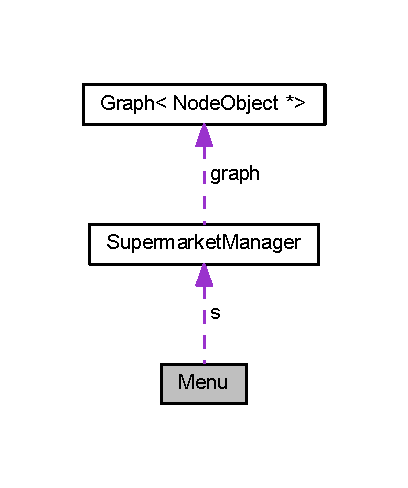
\includegraphics[width=196pt]{class_menu__coll__graph}
\end{center}
\end{figure}
\subsection*{Public Member Functions}
\begin{DoxyCompactItemize}
\item 
\hyperlink{class_menu_a506d3403e4cc1ad520bdae62e14ae92e}{Menu} (\hyperlink{class_supermarket_manager}{Supermarket\+Manager} \hyperlink{class_menu_ae5304bdde33c0480b8dfc1427de00c5a}{s})
\item 
void \hyperlink{class_menu_aef9edee86d2ea460606361c92e061583}{main\+Menu} ()
\item 
void \hyperlink{class_menu_a8f6414360aee0273d3295ed3467bfaad}{deliver\+Menu} ()
\item 
void \hyperlink{class_menu_ac9b447341eeb69abc0c9862b5a5be1c1}{search\+Menu} ()
\end{DoxyCompactItemize}
\subsection*{Private Attributes}
\begin{DoxyCompactItemize}
\item 
\hyperlink{class_supermarket_manager}{Supermarket\+Manager} \hyperlink{class_menu_ae5304bdde33c0480b8dfc1427de00c5a}{s}
\end{DoxyCompactItemize}


\subsection{Constructor \& Destructor Documentation}
\mbox{\Hypertarget{class_menu_a506d3403e4cc1ad520bdae62e14ae92e}\label{class_menu_a506d3403e4cc1ad520bdae62e14ae92e}} 
\index{Menu@{Menu}!Menu@{Menu}}
\index{Menu@{Menu}!Menu@{Menu}}
\subsubsection{\texorpdfstring{Menu()}{Menu()}}
{\footnotesize\ttfamily Menu\+::\+Menu (\begin{DoxyParamCaption}\item[{\hyperlink{class_supermarket_manager}{Supermarket\+Manager}}]{s }\end{DoxyParamCaption})}

Construtor da classe \hyperlink{class_menu}{Menu}. Chama o metodo main\+Menu.


\begin{DoxyParams}{Parameters}
{\em s} & gestor de supermercados \\
\hline
\end{DoxyParams}
Here is the call graph for this function\+:
\nopagebreak
\begin{figure}[H]
\begin{center}
\leavevmode
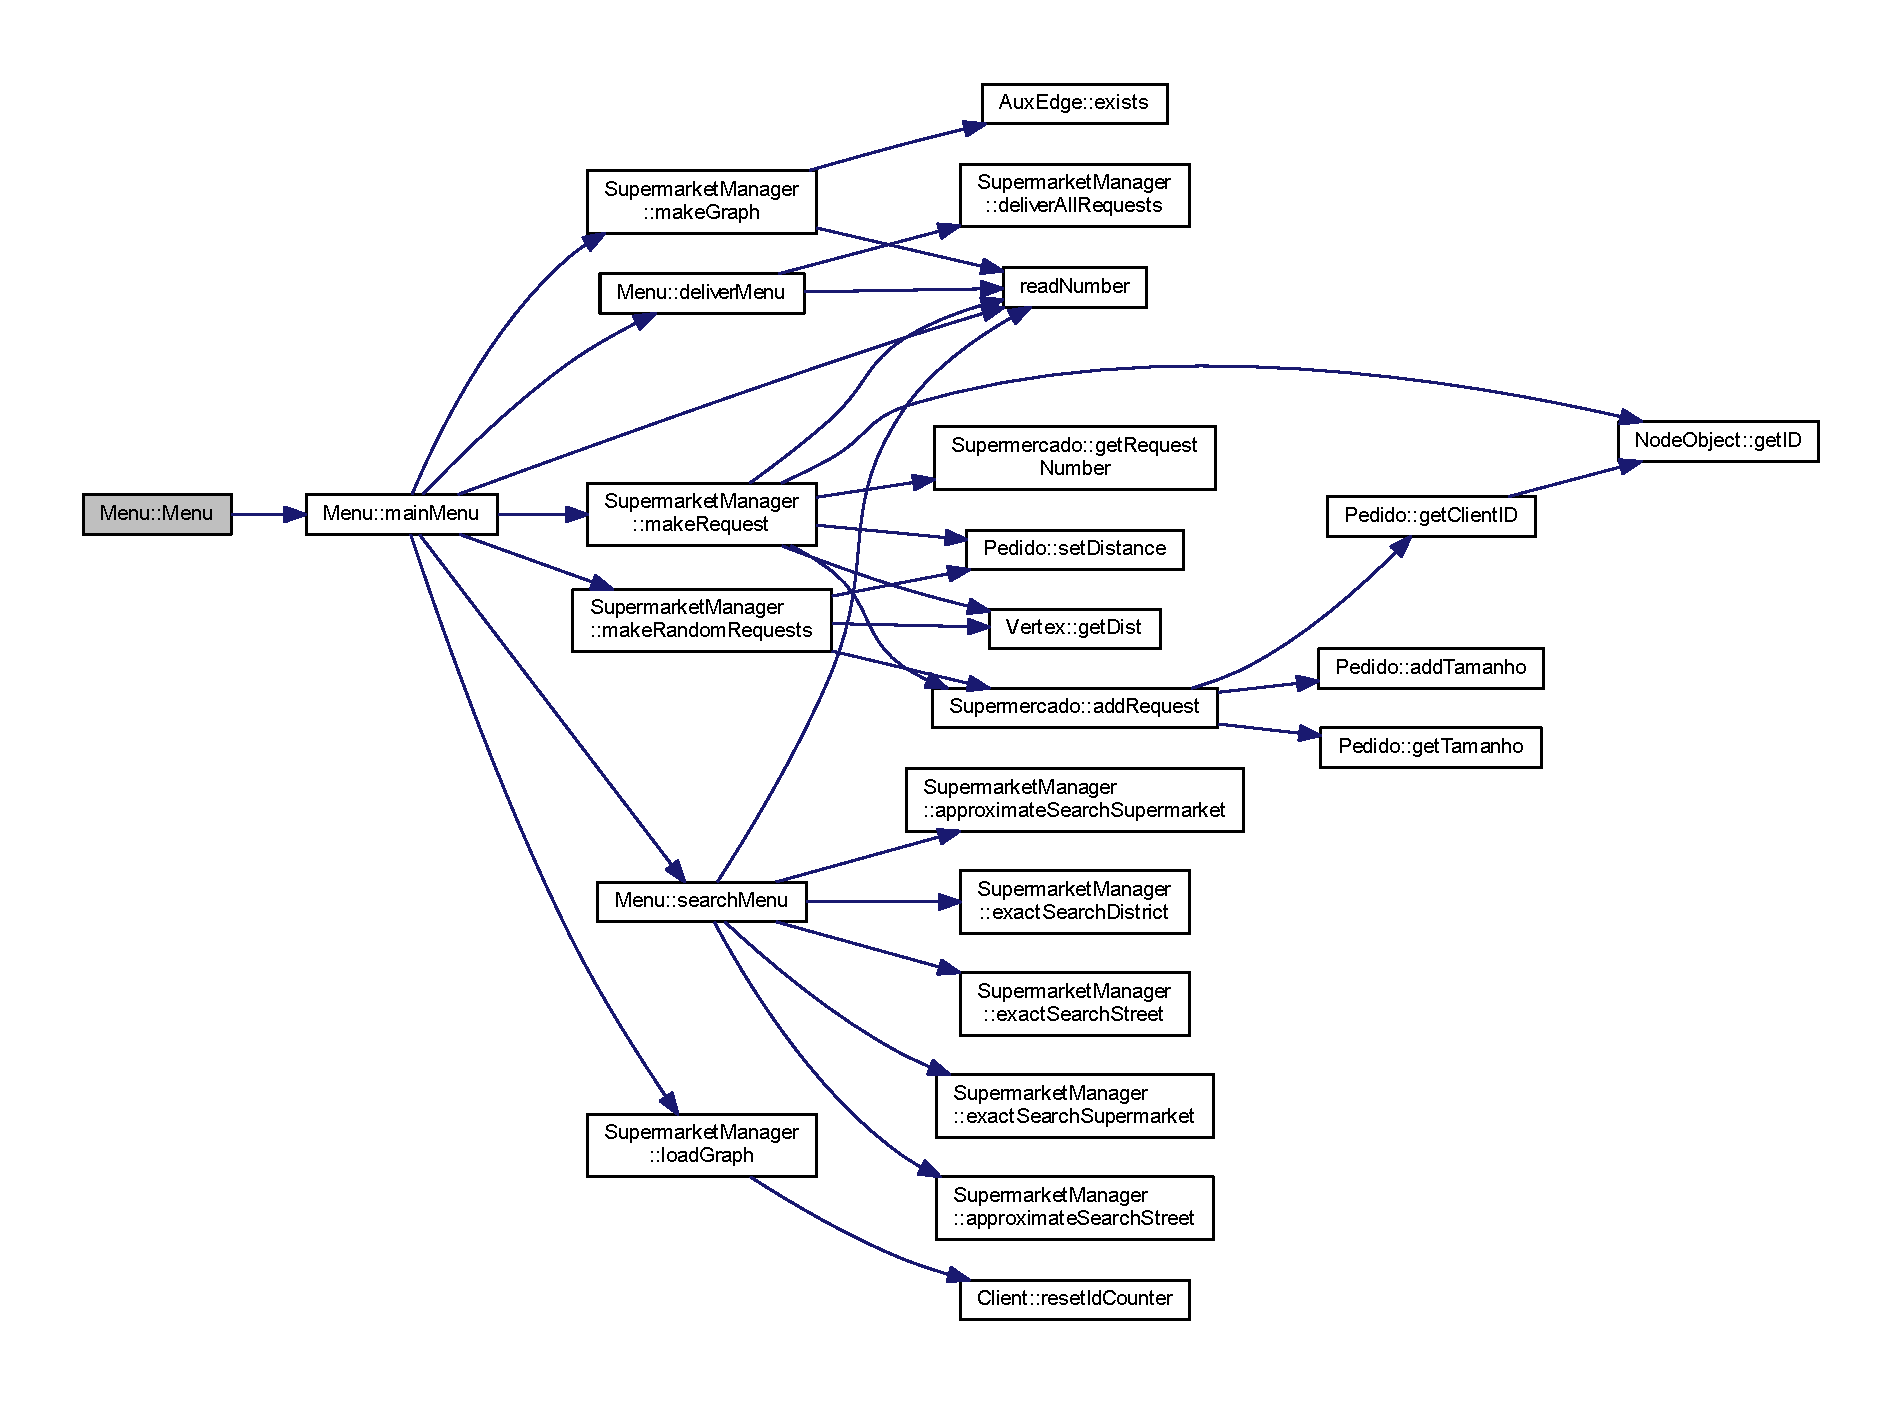
\includegraphics[width=350pt]{class_menu_a506d3403e4cc1ad520bdae62e14ae92e_cgraph}
\end{center}
\end{figure}


\subsection{Member Function Documentation}
\mbox{\Hypertarget{class_menu_a8f6414360aee0273d3295ed3467bfaad}\label{class_menu_a8f6414360aee0273d3295ed3467bfaad}} 
\index{Menu@{Menu}!deliver\+Menu@{deliver\+Menu}}
\index{deliver\+Menu@{deliver\+Menu}!Menu@{Menu}}
\subsubsection{\texorpdfstring{deliver\+Menu()}{deliverMenu()}}
{\footnotesize\ttfamily void Menu\+::deliver\+Menu (\begin{DoxyParamCaption}{ }\end{DoxyParamCaption})}

Funcao responsavel pelo menu de entrega de pedidos. Here is the call graph for this function\+:
\nopagebreak
\begin{figure}[H]
\begin{center}
\leavevmode
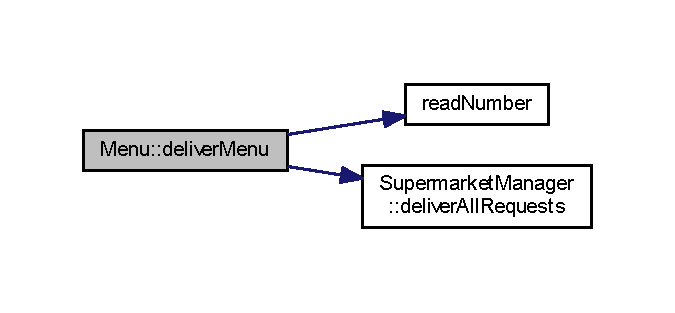
\includegraphics[width=324pt]{class_menu_a8f6414360aee0273d3295ed3467bfaad_cgraph}
\end{center}
\end{figure}
Here is the caller graph for this function\+:
\nopagebreak
\begin{figure}[H]
\begin{center}
\leavevmode
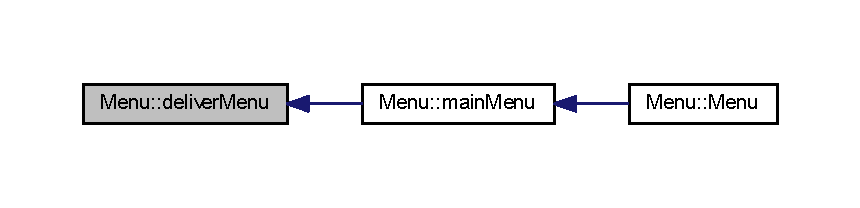
\includegraphics[width=350pt]{class_menu_a8f6414360aee0273d3295ed3467bfaad_icgraph}
\end{center}
\end{figure}
\mbox{\Hypertarget{class_menu_aef9edee86d2ea460606361c92e061583}\label{class_menu_aef9edee86d2ea460606361c92e061583}} 
\index{Menu@{Menu}!main\+Menu@{main\+Menu}}
\index{main\+Menu@{main\+Menu}!Menu@{Menu}}
\subsubsection{\texorpdfstring{main\+Menu()}{mainMenu()}}
{\footnotesize\ttfamily void Menu\+::main\+Menu (\begin{DoxyParamCaption}{ }\end{DoxyParamCaption})}

Funcao responsavel pelo menu principal do programa. Here is the call graph for this function\+:
\nopagebreak
\begin{figure}[H]
\begin{center}
\leavevmode
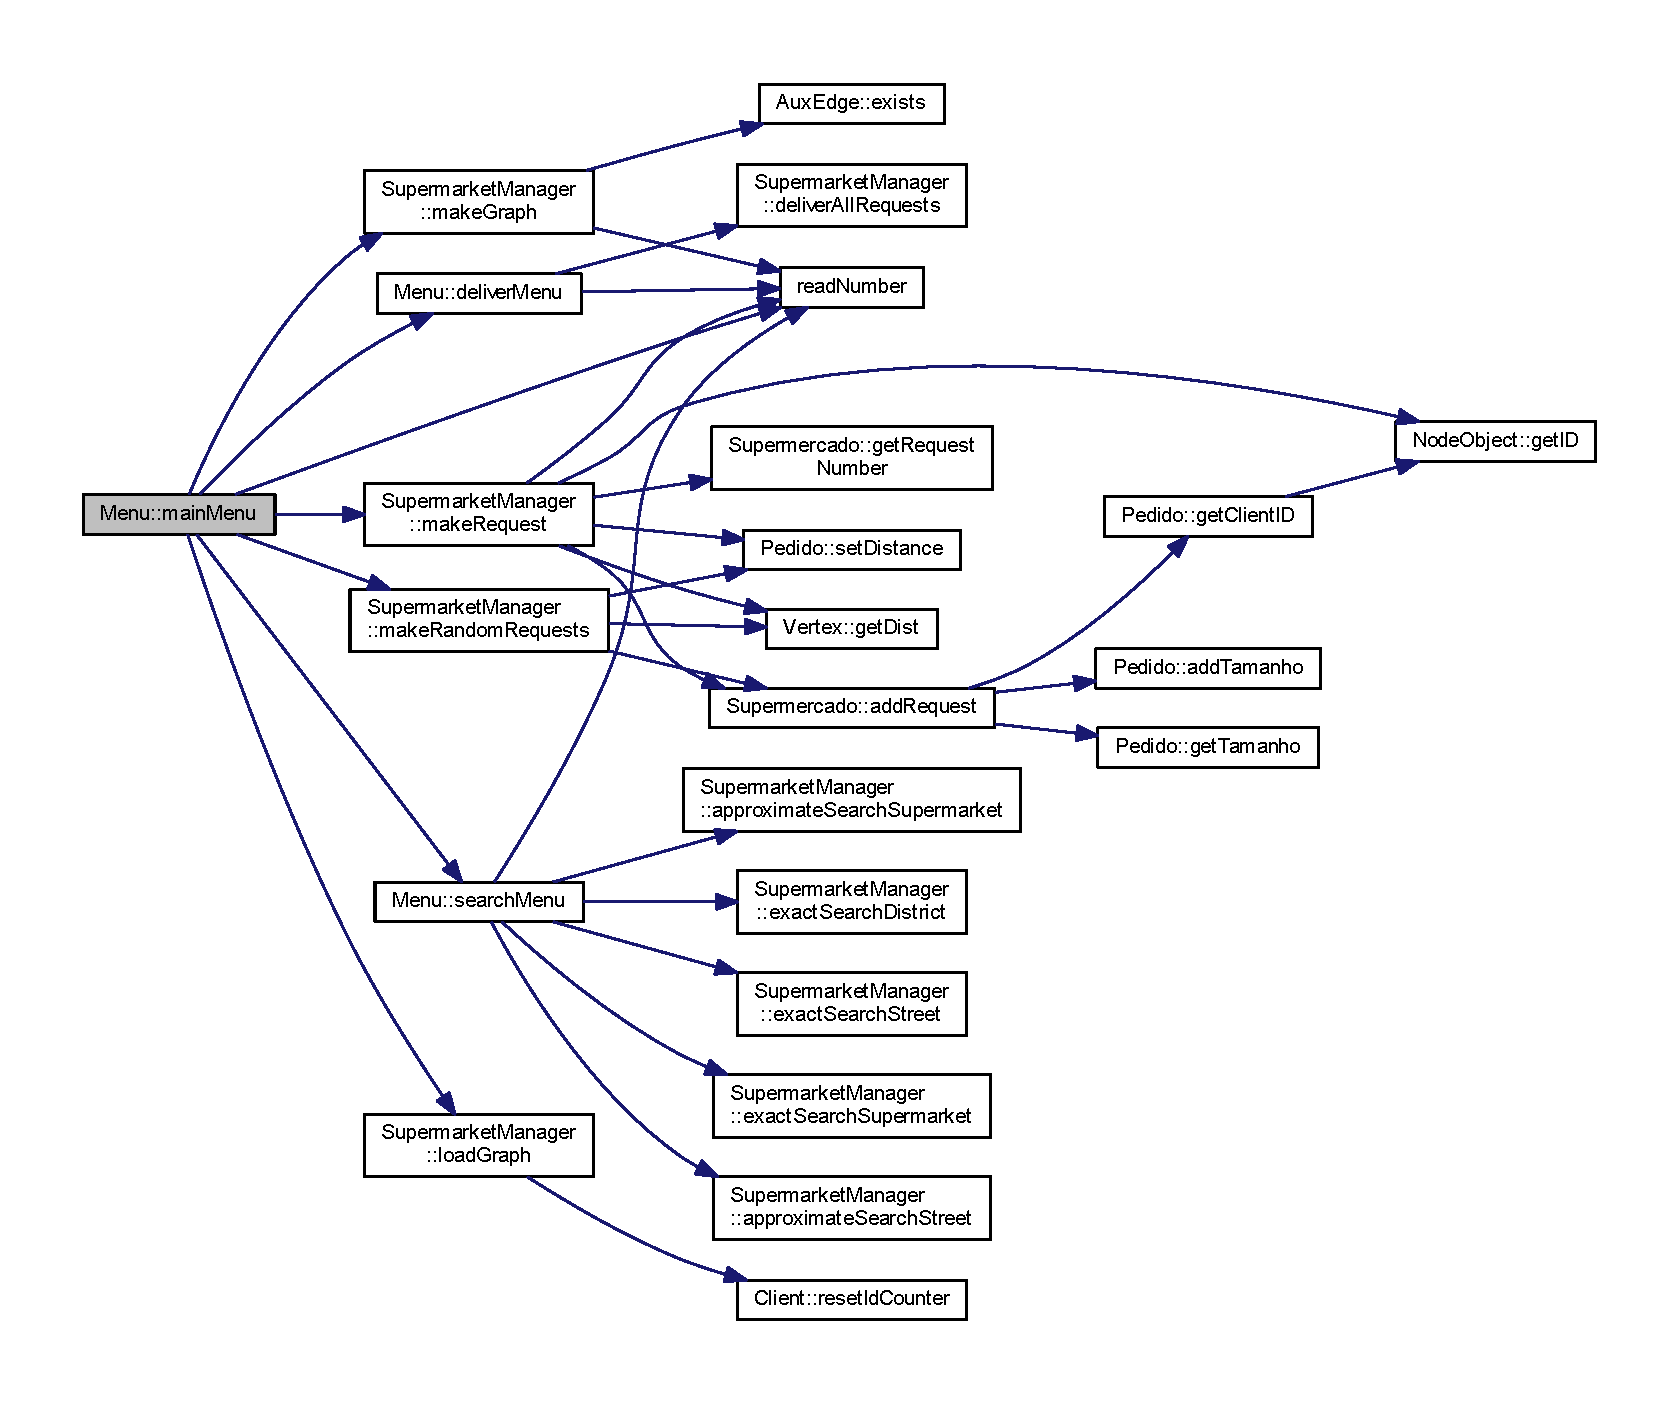
\includegraphics[width=350pt]{class_menu_aef9edee86d2ea460606361c92e061583_cgraph}
\end{center}
\end{figure}
Here is the caller graph for this function\+:
\nopagebreak
\begin{figure}[H]
\begin{center}
\leavevmode
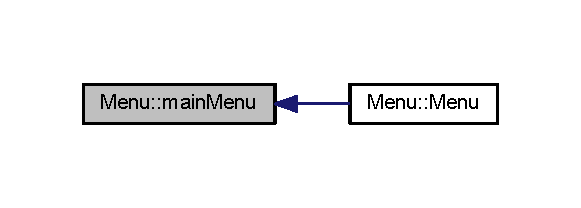
\includegraphics[width=279pt]{class_menu_aef9edee86d2ea460606361c92e061583_icgraph}
\end{center}
\end{figure}
\mbox{\Hypertarget{class_menu_ac9b447341eeb69abc0c9862b5a5be1c1}\label{class_menu_ac9b447341eeb69abc0c9862b5a5be1c1}} 
\index{Menu@{Menu}!search\+Menu@{search\+Menu}}
\index{search\+Menu@{search\+Menu}!Menu@{Menu}}
\subsubsection{\texorpdfstring{search\+Menu()}{searchMenu()}}
{\footnotesize\ttfamily void Menu\+::search\+Menu (\begin{DoxyParamCaption}{ }\end{DoxyParamCaption})}

Funcao responsavel pelo menu de pesquisa. Here is the call graph for this function\+:
\nopagebreak
\begin{figure}[H]
\begin{center}
\leavevmode
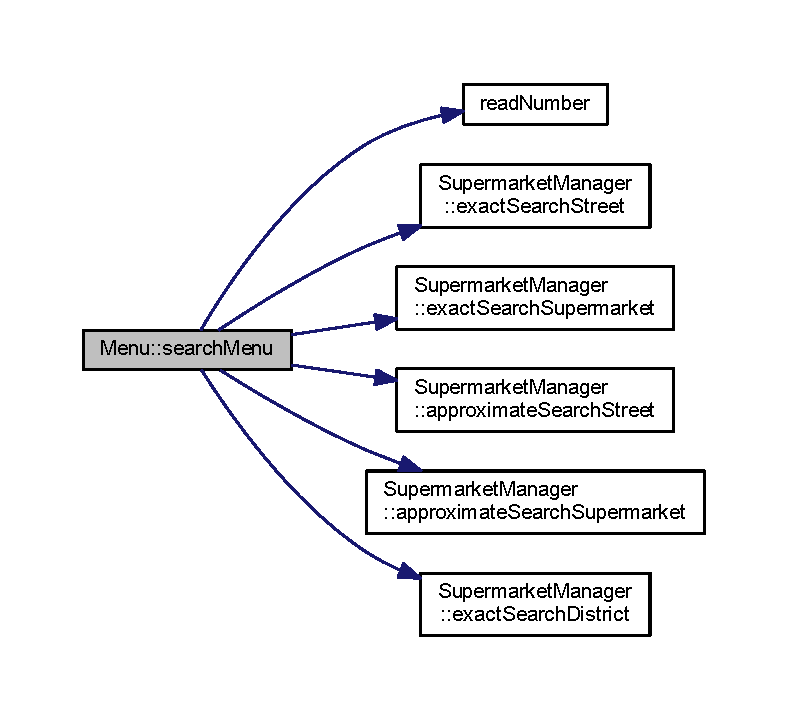
\includegraphics[width=350pt]{class_menu_ac9b447341eeb69abc0c9862b5a5be1c1_cgraph}
\end{center}
\end{figure}
Here is the caller graph for this function\+:
\nopagebreak
\begin{figure}[H]
\begin{center}
\leavevmode
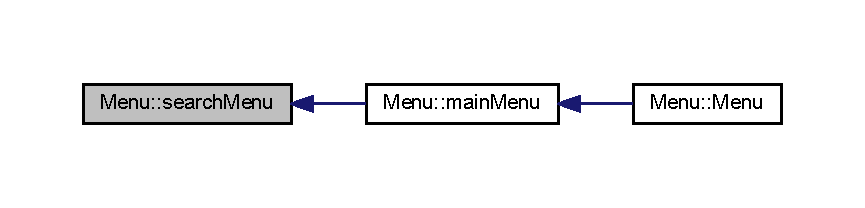
\includegraphics[width=350pt]{class_menu_ac9b447341eeb69abc0c9862b5a5be1c1_icgraph}
\end{center}
\end{figure}


\subsection{Member Data Documentation}
\mbox{\Hypertarget{class_menu_ae5304bdde33c0480b8dfc1427de00c5a}\label{class_menu_ae5304bdde33c0480b8dfc1427de00c5a}} 
\index{Menu@{Menu}!s@{s}}
\index{s@{s}!Menu@{Menu}}
\subsubsection{\texorpdfstring{s}{s}}
{\footnotesize\ttfamily \hyperlink{class_supermarket_manager}{Supermarket\+Manager} Menu\+::s\hspace{0.3cm}{\ttfamily [private]}}

Este atributo � o gestor de uma cadeia de supermercados sobre o qual o menu vai operar. 

The documentation for this class was generated from the following files\+:\begin{DoxyCompactItemize}
\item 
\hyperlink{_menu_8h}{Menu.\+h}\item 
\hyperlink{_menu_8cpp}{Menu.\+cpp}\end{DoxyCompactItemize}

\hypertarget{class_node_object}{}\section{Node\+Object Class Reference}
\label{class_node_object}\index{Node\+Object@{Node\+Object}}


{\ttfamily \#include $<$Node\+Object.\+h$>$}



Inheritance diagram for Node\+Object\+:
\nopagebreak
\begin{figure}[H]
\begin{center}
\leavevmode
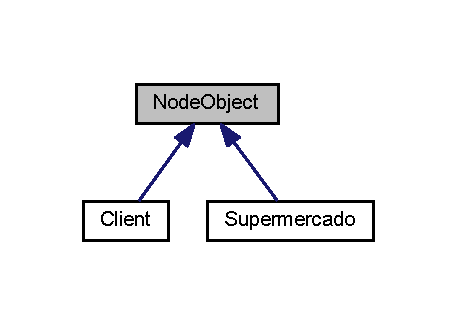
\includegraphics[width=220pt]{class_node_object__inherit__graph}
\end{center}
\end{figure}
\subsection*{Public Member Functions}
\begin{DoxyCompactItemize}
\item 
\hyperlink{class_node_object_a7ea385aba27682c7be7c3028f78476af}{Node\+Object} ()
\item 
int \hyperlink{class_node_object_a42a10492f5acabd11e544b19cfc365ab}{get\+ID} ()
\item 
string \hyperlink{class_node_object_a472240f1f5cd59583cacddadda08036b}{get\+Distrito} ()
\item 
bool \hyperlink{class_node_object_a2808f33e6c6897ab18372fe5636ce05f}{operator==} (const \hyperlink{class_node_object}{Node\+Object} \&rhs)
\end{DoxyCompactItemize}
\subsection*{Static Protected Attributes}
\begin{DoxyCompactItemize}
\item 
static int \hyperlink{class_node_object_ac87a713167757cef78d75242b18c25ed}{id\+\_\+counter} = 0
\end{DoxyCompactItemize}
\subsection*{Private Attributes}
\begin{DoxyCompactItemize}
\item 
int \hyperlink{class_node_object_ace7dd5d8d02ead5f64b8ba59109ba9c6}{id}
\item 
string \hyperlink{class_node_object_acff2ecbe7ba33bd7b9ce1eef79658138}{distrito}
\end{DoxyCompactItemize}


\subsection{Constructor \& Destructor Documentation}
\mbox{\Hypertarget{class_node_object_a7ea385aba27682c7be7c3028f78476af}\label{class_node_object_a7ea385aba27682c7be7c3028f78476af}} 
\index{Node\+Object@{Node\+Object}!Node\+Object@{Node\+Object}}
\index{Node\+Object@{Node\+Object}!Node\+Object@{Node\+Object}}
\subsubsection{\texorpdfstring{Node\+Object()}{NodeObject()}}
{\footnotesize\ttfamily Node\+Object\+::\+Node\+Object (\begin{DoxyParamCaption}{ }\end{DoxyParamCaption})}

Construtor por omissao de um n�. 

\subsection{Member Function Documentation}
\mbox{\Hypertarget{class_node_object_a472240f1f5cd59583cacddadda08036b}\label{class_node_object_a472240f1f5cd59583cacddadda08036b}} 
\index{Node\+Object@{Node\+Object}!get\+Distrito@{get\+Distrito}}
\index{get\+Distrito@{get\+Distrito}!Node\+Object@{Node\+Object}}
\subsubsection{\texorpdfstring{get\+Distrito()}{getDistrito()}}
{\footnotesize\ttfamily string Node\+Object\+::get\+Distrito (\begin{DoxyParamCaption}{ }\end{DoxyParamCaption})}

Retorna o distrito do no

\begin{DoxyReturn}{Returns}
distrito do no 
\end{DoxyReturn}
\mbox{\Hypertarget{class_node_object_a42a10492f5acabd11e544b19cfc365ab}\label{class_node_object_a42a10492f5acabd11e544b19cfc365ab}} 
\index{Node\+Object@{Node\+Object}!get\+ID@{get\+ID}}
\index{get\+ID@{get\+ID}!Node\+Object@{Node\+Object}}
\subsubsection{\texorpdfstring{get\+I\+D()}{getID()}}
{\footnotesize\ttfamily int Node\+Object\+::get\+ID (\begin{DoxyParamCaption}{ }\end{DoxyParamCaption})}

Retorna o ID do n�

\begin{DoxyReturn}{Returns}
ID do n� 
\end{DoxyReturn}
Here is the caller graph for this function\+:
\nopagebreak
\begin{figure}[H]
\begin{center}
\leavevmode
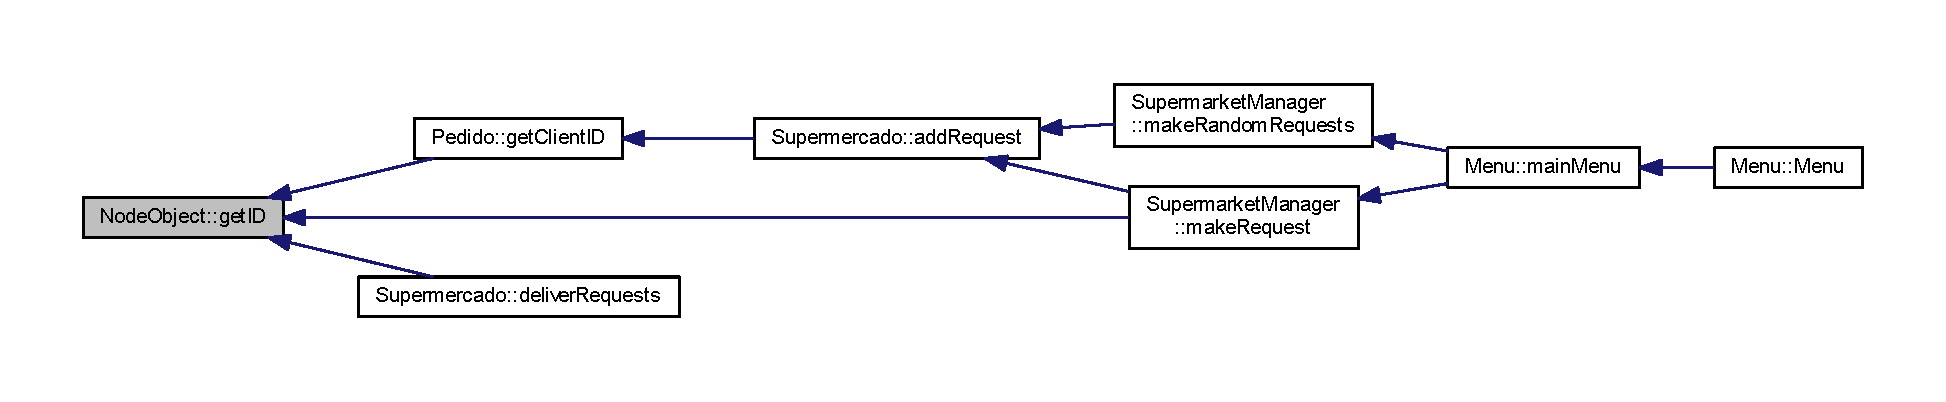
\includegraphics[width=350pt]{class_node_object_a42a10492f5acabd11e544b19cfc365ab_icgraph}
\end{center}
\end{figure}
\mbox{\Hypertarget{class_node_object_a2808f33e6c6897ab18372fe5636ce05f}\label{class_node_object_a2808f33e6c6897ab18372fe5636ce05f}} 
\index{Node\+Object@{Node\+Object}!operator==@{operator==}}
\index{operator==@{operator==}!Node\+Object@{Node\+Object}}
\subsubsection{\texorpdfstring{operator==()}{operator==()}}
{\footnotesize\ttfamily bool Node\+Object\+::operator== (\begin{DoxyParamCaption}\item[{const \hyperlink{class_node_object}{Node\+Object} \&}]{rhs }\end{DoxyParamCaption})}

Operador de igualde de n�s. Um n� � igual a outro se tiverem o mesmo ID. 

\subsection{Member Data Documentation}
\mbox{\Hypertarget{class_node_object_acff2ecbe7ba33bd7b9ce1eef79658138}\label{class_node_object_acff2ecbe7ba33bd7b9ce1eef79658138}} 
\index{Node\+Object@{Node\+Object}!distrito@{distrito}}
\index{distrito@{distrito}!Node\+Object@{Node\+Object}}
\subsubsection{\texorpdfstring{distrito}{distrito}}
{\footnotesize\ttfamily string Node\+Object\+::distrito\hspace{0.3cm}{\ttfamily [private]}}

Distrito onde se localiza o no \mbox{\Hypertarget{class_node_object_ace7dd5d8d02ead5f64b8ba59109ba9c6}\label{class_node_object_ace7dd5d8d02ead5f64b8ba59109ba9c6}} 
\index{Node\+Object@{Node\+Object}!id@{id}}
\index{id@{id}!Node\+Object@{Node\+Object}}
\subsubsection{\texorpdfstring{id}{id}}
{\footnotesize\ttfamily int Node\+Object\+::id\hspace{0.3cm}{\ttfamily [private]}}

Identificador �nico de um n�. \mbox{\Hypertarget{class_node_object_ac87a713167757cef78d75242b18c25ed}\label{class_node_object_ac87a713167757cef78d75242b18c25ed}} 
\index{Node\+Object@{Node\+Object}!id\+\_\+counter@{id\+\_\+counter}}
\index{id\+\_\+counter@{id\+\_\+counter}!Node\+Object@{Node\+Object}}
\subsubsection{\texorpdfstring{id\+\_\+counter}{id\_counter}}
{\footnotesize\ttfamily int Node\+Object\+::id\+\_\+counter = 0\hspace{0.3cm}{\ttfamily [static]}, {\ttfamily [protected]}}

Contador sequencial dos I\+Ds dos n�s (clientes e supermercados). 

The documentation for this class was generated from the following files\+:\begin{DoxyCompactItemize}
\item 
\hyperlink{_node_object_8h}{Node\+Object.\+h}\item 
\hyperlink{_node_object_8cpp}{Node\+Object.\+cpp}\end{DoxyCompactItemize}

\hypertarget{class_pedido}{}\section{Pedido Class Reference}
\label{class_pedido}\index{Pedido@{Pedido}}


{\ttfamily \#include $<$Pedido.\+h$>$}



Collaboration diagram for Pedido\+:
\nopagebreak
\begin{figure}[H]
\begin{center}
\leavevmode
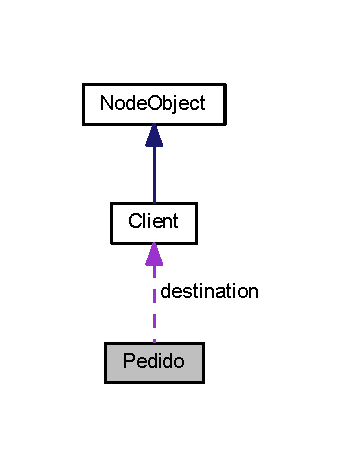
\includegraphics[width=165pt]{class_pedido__coll__graph}
\end{center}
\end{figure}
\subsection*{Public Member Functions}
\begin{DoxyCompactItemize}
\item 
\hyperlink{class_pedido_a674084f1803ef97e5a4a03fc2651bde0}{Pedido} (\hyperlink{class_client}{Client} $\ast$\hyperlink{class_pedido_ab23e35be8be8b757ca81b1ef65c21717}{destination}, int \hyperlink{class_pedido_aeb8dc710976c78607a68485523a67cec}{tamanho})
\item 
int \hyperlink{class_pedido_a06797f0a6137df4f27a6602af083cdde}{get\+Client\+ID} ()
\item 
\hyperlink{class_client}{Client} $\ast$ \hyperlink{class_pedido_accbdb24c3c528262a713fd5da5e8af4a}{get\+Destination} ()
\item 
int \hyperlink{class_pedido_a4eb7ace45204e2c8c90c9e252833eca2}{get\+Tamanho} ()
\item 
void \hyperlink{class_pedido_a4779b145a7fba66eb5d3c9510ffe1adb}{set\+Tamanho} (int \hyperlink{class_pedido_aeb8dc710976c78607a68485523a67cec}{tamanho})
\item 
void \hyperlink{class_pedido_a728b4d0fb30b07498a18b28d92079abe}{add\+Tamanho} (int incremento)
\item 
int \hyperlink{class_pedido_acdb1147bb5d2c89d1076b40a9de4ce90}{get\+Distance} ()
\item 
void \hyperlink{class_pedido_a4c93021f91deafdf3e0e05fd26e2fa5d}{set\+Distance} (int \hyperlink{class_pedido_a5eb76f039a131307b89e56bc2c8aee0c}{distance})
\end{DoxyCompactItemize}
\subsection*{Private Attributes}
\begin{DoxyCompactItemize}
\item 
\hyperlink{class_client}{Client} $\ast$ \hyperlink{class_pedido_ab23e35be8be8b757ca81b1ef65c21717}{destination}
\item 
int \hyperlink{class_pedido_aeb8dc710976c78607a68485523a67cec}{tamanho} = 0
\item 
int \hyperlink{class_pedido_a5eb76f039a131307b89e56bc2c8aee0c}{distance} = \hyperlink{_graph_8h_a9fff7b07b84324efa12018456a60d91b}{I\+N\+T\+\_\+\+I\+N\+F\+I\+N\+I\+TY}
\end{DoxyCompactItemize}


\subsection{Constructor \& Destructor Documentation}
\mbox{\Hypertarget{class_pedido_a674084f1803ef97e5a4a03fc2651bde0}\label{class_pedido_a674084f1803ef97e5a4a03fc2651bde0}} 
\index{Pedido@{Pedido}!Pedido@{Pedido}}
\index{Pedido@{Pedido}!Pedido@{Pedido}}
\subsubsection{\texorpdfstring{Pedido()}{Pedido()}}
{\footnotesize\ttfamily Pedido\+::\+Pedido (\begin{DoxyParamCaption}\item[{\hyperlink{class_client}{Client} $\ast$}]{destination,  }\item[{int}]{tamanho }\end{DoxyParamCaption})\hspace{0.3cm}{\ttfamily [inline]}}

Contrutor do pedido.


\begin{DoxyParams}{Parameters}
{\em destination} & cliente que efetuou o pedido \\
\hline
{\em tamanho} & tamanho do pedido \\
\hline
\end{DoxyParams}


\subsection{Member Function Documentation}
\mbox{\Hypertarget{class_pedido_a728b4d0fb30b07498a18b28d92079abe}\label{class_pedido_a728b4d0fb30b07498a18b28d92079abe}} 
\index{Pedido@{Pedido}!add\+Tamanho@{add\+Tamanho}}
\index{add\+Tamanho@{add\+Tamanho}!Pedido@{Pedido}}
\subsubsection{\texorpdfstring{add\+Tamanho()}{addTamanho()}}
{\footnotesize\ttfamily void Pedido\+::add\+Tamanho (\begin{DoxyParamCaption}\item[{int}]{incremento }\end{DoxyParamCaption})\hspace{0.3cm}{\ttfamily [inline]}}

Soma um valor ao tamanho do pedido. Se esta opera��o exceder a capacidade maxima definida para os pedidos, o pedido ficar� com o tamanho m�ximo.


\begin{DoxyParams}{Parameters}
{\em incremento} & valor a somar ao tamanho do pedido \\
\hline
\end{DoxyParams}
Here is the caller graph for this function\+:
\nopagebreak
\begin{figure}[H]
\begin{center}
\leavevmode
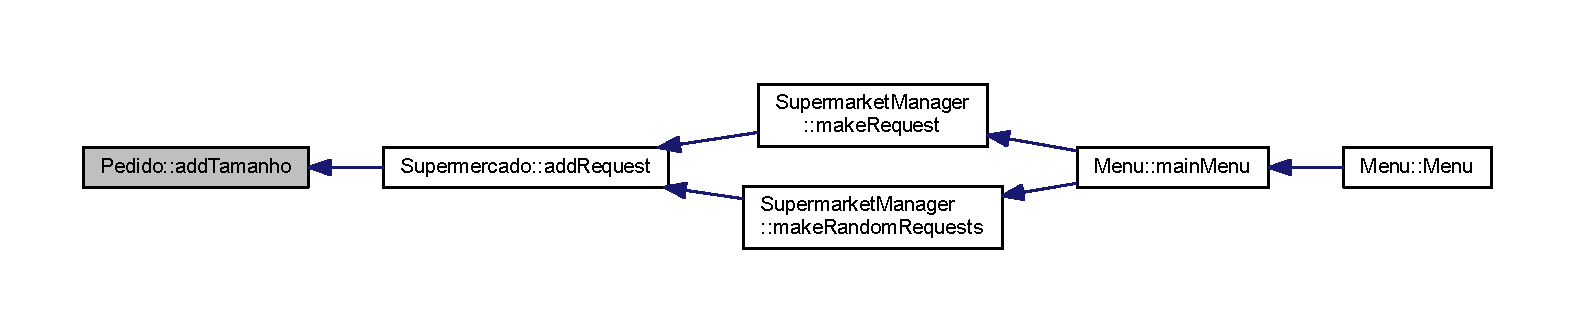
\includegraphics[width=350pt]{class_pedido_a728b4d0fb30b07498a18b28d92079abe_icgraph}
\end{center}
\end{figure}
\mbox{\Hypertarget{class_pedido_a06797f0a6137df4f27a6602af083cdde}\label{class_pedido_a06797f0a6137df4f27a6602af083cdde}} 
\index{Pedido@{Pedido}!get\+Client\+ID@{get\+Client\+ID}}
\index{get\+Client\+ID@{get\+Client\+ID}!Pedido@{Pedido}}
\subsubsection{\texorpdfstring{get\+Client\+I\+D()}{getClientID()}}
{\footnotesize\ttfamily int Pedido\+::get\+Client\+ID (\begin{DoxyParamCaption}{ }\end{DoxyParamCaption})\hspace{0.3cm}{\ttfamily [inline]}}

Retorna o ID do cliente que fez o pedido

\begin{DoxyReturn}{Returns}
o ID do cliente que fez o pedido 
\end{DoxyReturn}
Here is the call graph for this function\+:
\nopagebreak
\begin{figure}[H]
\begin{center}
\leavevmode
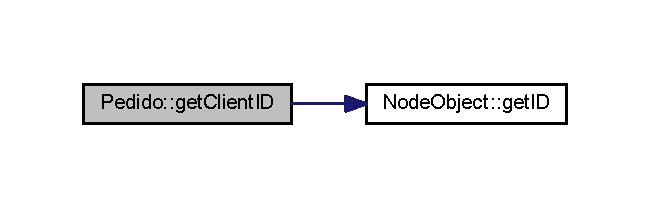
\includegraphics[width=312pt]{class_pedido_a06797f0a6137df4f27a6602af083cdde_cgraph}
\end{center}
\end{figure}
Here is the caller graph for this function\+:
\nopagebreak
\begin{figure}[H]
\begin{center}
\leavevmode
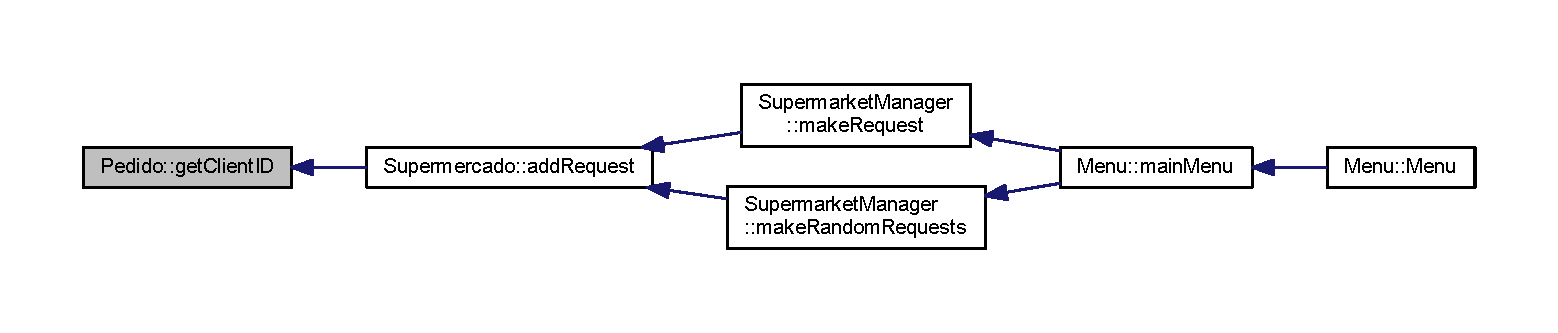
\includegraphics[width=350pt]{class_pedido_a06797f0a6137df4f27a6602af083cdde_icgraph}
\end{center}
\end{figure}
\mbox{\Hypertarget{class_pedido_accbdb24c3c528262a713fd5da5e8af4a}\label{class_pedido_accbdb24c3c528262a713fd5da5e8af4a}} 
\index{Pedido@{Pedido}!get\+Destination@{get\+Destination}}
\index{get\+Destination@{get\+Destination}!Pedido@{Pedido}}
\subsubsection{\texorpdfstring{get\+Destination()}{getDestination()}}
{\footnotesize\ttfamily \hyperlink{class_client}{Client}$\ast$ Pedido\+::get\+Destination (\begin{DoxyParamCaption}{ }\end{DoxyParamCaption})\hspace{0.3cm}{\ttfamily [inline]}}

Retorna um apontador para o cliente que fez o pedido

\begin{DoxyReturn}{Returns}
um apontador para o cliente que fez o pedido 
\end{DoxyReturn}
Here is the caller graph for this function\+:
\nopagebreak
\begin{figure}[H]
\begin{center}
\leavevmode
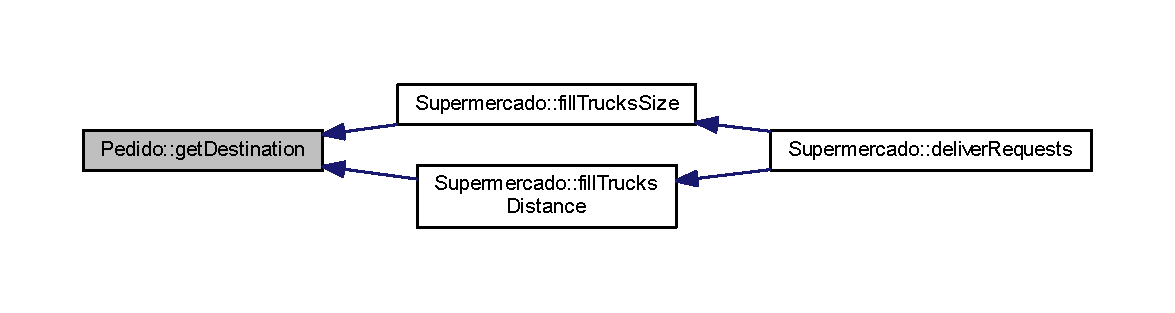
\includegraphics[width=350pt]{class_pedido_accbdb24c3c528262a713fd5da5e8af4a_icgraph}
\end{center}
\end{figure}
\mbox{\Hypertarget{class_pedido_acdb1147bb5d2c89d1076b40a9de4ce90}\label{class_pedido_acdb1147bb5d2c89d1076b40a9de4ce90}} 
\index{Pedido@{Pedido}!get\+Distance@{get\+Distance}}
\index{get\+Distance@{get\+Distance}!Pedido@{Pedido}}
\subsubsection{\texorpdfstring{get\+Distance()}{getDistance()}}
{\footnotesize\ttfamily int Pedido\+::get\+Distance (\begin{DoxyParamCaption}{ }\end{DoxyParamCaption})\hspace{0.3cm}{\ttfamily [inline]}}

Retorna a distancia do cliente que efetuou o pedido ao supermercado encarregue pelo mesmo.

\begin{DoxyReturn}{Returns}
distancia do cliente que efetuou o pedido ao supermercado encarregue pelo mesmo. 
\end{DoxyReturn}
Here is the caller graph for this function\+:
\nopagebreak
\begin{figure}[H]
\begin{center}
\leavevmode
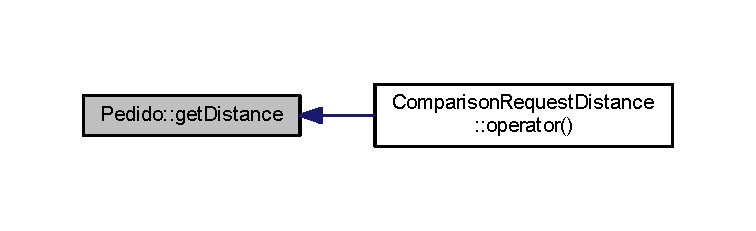
\includegraphics[width=350pt]{class_pedido_acdb1147bb5d2c89d1076b40a9de4ce90_icgraph}
\end{center}
\end{figure}
\mbox{\Hypertarget{class_pedido_a4eb7ace45204e2c8c90c9e252833eca2}\label{class_pedido_a4eb7ace45204e2c8c90c9e252833eca2}} 
\index{Pedido@{Pedido}!get\+Tamanho@{get\+Tamanho}}
\index{get\+Tamanho@{get\+Tamanho}!Pedido@{Pedido}}
\subsubsection{\texorpdfstring{get\+Tamanho()}{getTamanho()}}
{\footnotesize\ttfamily int Pedido\+::get\+Tamanho (\begin{DoxyParamCaption}{ }\end{DoxyParamCaption})\hspace{0.3cm}{\ttfamily [inline]}}

Retorna o tamanho do pedido

\begin{DoxyReturn}{Returns}
o tamanho do pedido 
\end{DoxyReturn}
Here is the caller graph for this function\+:
\nopagebreak
\begin{figure}[H]
\begin{center}
\leavevmode
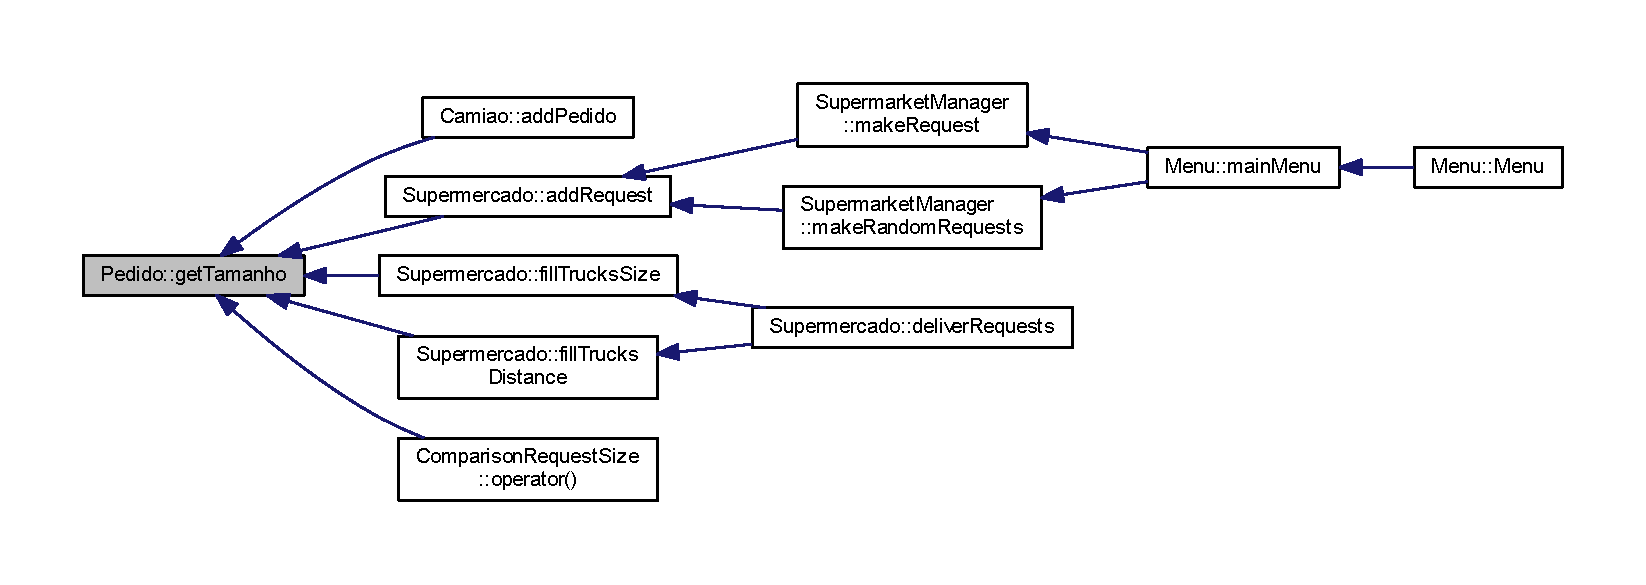
\includegraphics[width=350pt]{class_pedido_a4eb7ace45204e2c8c90c9e252833eca2_icgraph}
\end{center}
\end{figure}
\mbox{\Hypertarget{class_pedido_a4c93021f91deafdf3e0e05fd26e2fa5d}\label{class_pedido_a4c93021f91deafdf3e0e05fd26e2fa5d}} 
\index{Pedido@{Pedido}!set\+Distance@{set\+Distance}}
\index{set\+Distance@{set\+Distance}!Pedido@{Pedido}}
\subsubsection{\texorpdfstring{set\+Distance()}{setDistance()}}
{\footnotesize\ttfamily void Pedido\+::set\+Distance (\begin{DoxyParamCaption}\item[{int}]{distance }\end{DoxyParamCaption})\hspace{0.3cm}{\ttfamily [inline]}}

Atribui um valor inteiro � distancia do pedido.


\begin{DoxyParams}{Parameters}
{\em distance} & valor a atribuir � distancia do pedido \\
\hline
\end{DoxyParams}
Here is the caller graph for this function\+:
\nopagebreak
\begin{figure}[H]
\begin{center}
\leavevmode
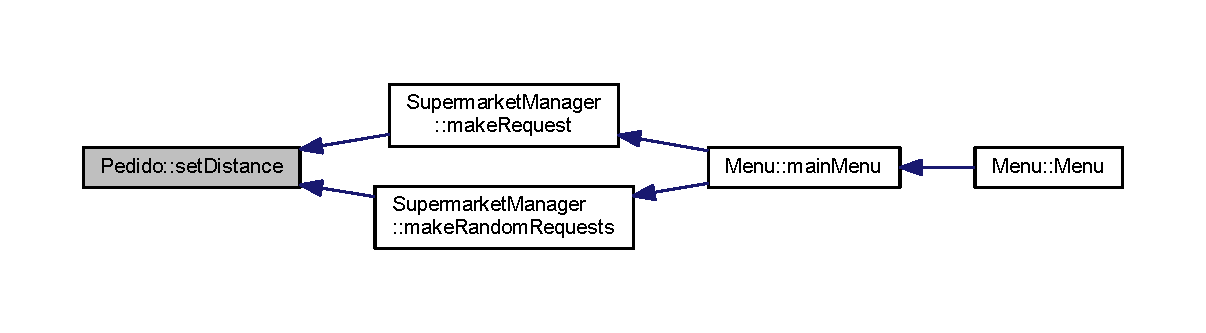
\includegraphics[width=350pt]{class_pedido_a4c93021f91deafdf3e0e05fd26e2fa5d_icgraph}
\end{center}
\end{figure}
\mbox{\Hypertarget{class_pedido_a4779b145a7fba66eb5d3c9510ffe1adb}\label{class_pedido_a4779b145a7fba66eb5d3c9510ffe1adb}} 
\index{Pedido@{Pedido}!set\+Tamanho@{set\+Tamanho}}
\index{set\+Tamanho@{set\+Tamanho}!Pedido@{Pedido}}
\subsubsection{\texorpdfstring{set\+Tamanho()}{setTamanho()}}
{\footnotesize\ttfamily void Pedido\+::set\+Tamanho (\begin{DoxyParamCaption}\item[{int}]{tamanho }\end{DoxyParamCaption})\hspace{0.3cm}{\ttfamily [inline]}}

Atribui um valor inteiro ao tamanho do pedido.


\begin{DoxyParams}{Parameters}
{\em tamanho} & valor a atribuir ao tamanho do pedido \\
\hline
\end{DoxyParams}


\subsection{Member Data Documentation}
\mbox{\Hypertarget{class_pedido_ab23e35be8be8b757ca81b1ef65c21717}\label{class_pedido_ab23e35be8be8b757ca81b1ef65c21717}} 
\index{Pedido@{Pedido}!destination@{destination}}
\index{destination@{destination}!Pedido@{Pedido}}
\subsubsection{\texorpdfstring{destination}{destination}}
{\footnotesize\ttfamily \hyperlink{class_client}{Client}$\ast$ Pedido\+::destination\hspace{0.3cm}{\ttfamily [private]}}

Apontador para o cliente que efetuou o pedido. \mbox{\Hypertarget{class_pedido_a5eb76f039a131307b89e56bc2c8aee0c}\label{class_pedido_a5eb76f039a131307b89e56bc2c8aee0c}} 
\index{Pedido@{Pedido}!distance@{distance}}
\index{distance@{distance}!Pedido@{Pedido}}
\subsubsection{\texorpdfstring{distance}{distance}}
{\footnotesize\ttfamily int Pedido\+::distance = \hyperlink{_graph_8h_a9fff7b07b84324efa12018456a60d91b}{I\+N\+T\+\_\+\+I\+N\+F\+I\+N\+I\+TY}\hspace{0.3cm}{\ttfamily [private]}}

Distancia do cliente que efetuou o pedido ao supermercado encarregue pelo mesmo. \mbox{\Hypertarget{class_pedido_aeb8dc710976c78607a68485523a67cec}\label{class_pedido_aeb8dc710976c78607a68485523a67cec}} 
\index{Pedido@{Pedido}!tamanho@{tamanho}}
\index{tamanho@{tamanho}!Pedido@{Pedido}}
\subsubsection{\texorpdfstring{tamanho}{tamanho}}
{\footnotesize\ttfamily int Pedido\+::tamanho = 0\hspace{0.3cm}{\ttfamily [private]}}

Tamanho do pedido. 

The documentation for this class was generated from the following file\+:\begin{DoxyCompactItemize}
\item 
\hyperlink{_pedido_8h}{Pedido.\+h}\end{DoxyCompactItemize}

\hypertarget{class_supermarket_manager}{}\section{Supermarket\+Manager Class Reference}
\label{class_supermarket_manager}\index{Supermarket\+Manager@{Supermarket\+Manager}}


{\ttfamily \#include $<$Supermarket\+Manager.\+h$>$}



Collaboration diagram for Supermarket\+Manager\+:
\nopagebreak
\begin{figure}[H]
\begin{center}
\leavevmode
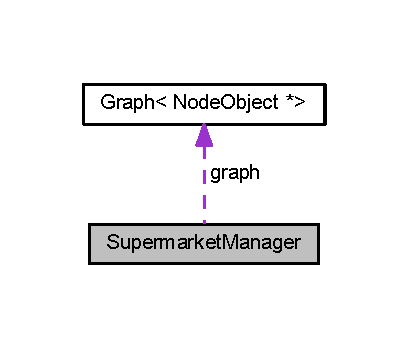
\includegraphics[width=196pt]{class_supermarket_manager__coll__graph}
\end{center}
\end{figure}
\subsection*{Public Member Functions}
\begin{DoxyCompactItemize}
\item 
\hyperlink{class_supermarket_manager_a32727a0b65ce19d2dddf66d586b0fa57}{Supermarket\+Manager} ()
\item 
void \hyperlink{class_supermarket_manager_a882d9161a59b259f5b0f62c230c11db9}{populate\+Graph} ()
\item 
void \hyperlink{class_supermarket_manager_abab275f63e6169a76efd92c90aaac0b4}{make\+Graph} ()
\item 
void \hyperlink{class_supermarket_manager_a0072988df7db4459fe0a409894af51a4}{load\+Graph} ()
\item 
\hyperlink{class_client}{Client} $\ast$ \hyperlink{class_supermarket_manager_a15c50e904600847775367ff4f626f62d}{get\+Client} (int id)
\item 
void \hyperlink{class_supermarket_manager_a19901c8d338b7579398373aeda62ecf2}{make\+Request} ()
\item 
void \hyperlink{class_supermarket_manager_a6dbf83eef3433341c7a971860e3b8915}{make\+Random\+Requests} ()
\item 
\hyperlink{class_supermercado}{Supermercado} $\ast$ \hyperlink{class_supermarket_manager_a3869489967f0a60d1b9c36a85b05998b}{find\+Nearest\+Supermarket} (\hyperlink{class_client}{Client} $\ast$client)
\item 
int \hyperlink{class_supermarket_manager_a45ed55914bea37bcf0d5757d1ce027c4}{input\+Client\+ID} ()
\item 
void \hyperlink{class_supermarket_manager_a034d77cc6da77516f6dbb4d6c3c0513d}{deliver\+All\+Requests} (int choice)
\item 
void \hyperlink{class_supermarket_manager_a3bbfc2db4c66bbaab3a5536c7205a818}{show\+Info} ()
\item 
void \hyperlink{class_supermarket_manager_a325c08bab73c6ddfe61dbb600c8d55fd}{strongly\+Connected\+Components} ()
\item 
bool \hyperlink{class_supermarket_manager_a6a688cb8cec4cc323cf4e53e04068c2c}{kmp\+Matcher} (string T, string P)
\item 
vector$<$ int $>$ \hyperlink{class_supermarket_manager_a3f18b0466fcb9369084ecd0c4e2d2e4a}{prefix\+Computation} (string P)
\item 
int \hyperlink{class_supermarket_manager_a16c8f9e3da09e91cb50d0ae932bb4eb2}{edit\+Distance} (string T, string P)
\item 
void \hyperlink{class_supermarket_manager_a23d192df8b8a56e317632845f9bb81d6}{check\+Supermarket\+Existence} (\hyperlink{class_edge}{Edge}$<$ \hyperlink{class_node_object}{Node\+Object} $\ast$$>$ e)
\item 
void \hyperlink{class_supermarket_manager_a7eca833133baf500e2a63b2ec9746b1d}{check\+Street} (\hyperlink{class_node_object}{Node\+Object} $\ast$market)
\item 
void \hyperlink{class_supermarket_manager_a7fa00d7adf078ca864908c901371a60c}{exact\+Search\+Street} ()
\item 
void \hyperlink{class_supermarket_manager_a0aa3fa8dab27db5f4960b840a2dd871c}{approximate\+Search\+Street} ()
\item 
void \hyperlink{class_supermarket_manager_a9841cd0c676abc1f128a68bb71bc2683}{exact\+Search\+Supermarket} ()
\item 
void \hyperlink{class_supermarket_manager_af797d69ada273a0582a619a0fc8f0638}{approximate\+Search\+Supermarket} ()
\item 
void \hyperlink{class_supermarket_manager_addbb66cfbe7d097687595c38e16b9c62}{exact\+Search\+District} ()
\end{DoxyCompactItemize}
\subsection*{Private Attributes}
\begin{DoxyCompactItemize}
\item 
\hyperlink{class_graph}{Graph}$<$ \hyperlink{class_node_object}{Node\+Object} $\ast$ $>$ \hyperlink{class_supermarket_manager_ab2cc638ffffc81beda833ca864e8bd62}{graph}
\item 
vector$<$ \hyperlink{class_client}{Client} $\ast$ $>$ \hyperlink{class_supermarket_manager_a48c5227a7d0ca5f8db9de726184e116a}{client\+List}
\item 
vector$<$ \hyperlink{class_supermercado}{Supermercado} $\ast$ $>$ \hyperlink{class_supermarket_manager_a122812406afbf7d0d130d39e6921d5f5}{market\+List}
\end{DoxyCompactItemize}


\subsection{Detailed Description}
Classe que gere uma cadeia de supermercados e os seus clientes 

\subsection{Constructor \& Destructor Documentation}
\mbox{\Hypertarget{class_supermarket_manager_a32727a0b65ce19d2dddf66d586b0fa57}\label{class_supermarket_manager_a32727a0b65ce19d2dddf66d586b0fa57}} 
\index{Supermarket\+Manager@{Supermarket\+Manager}!Supermarket\+Manager@{Supermarket\+Manager}}
\index{Supermarket\+Manager@{Supermarket\+Manager}!Supermarket\+Manager@{Supermarket\+Manager}}
\subsubsection{\texorpdfstring{Supermarket\+Manager()}{SupermarketManager()}}
{\footnotesize\ttfamily Supermarket\+Manager\+::\+Supermarket\+Manager (\begin{DoxyParamCaption}{ }\end{DoxyParamCaption})}

Construtor por omissao 

\subsection{Member Function Documentation}
\mbox{\Hypertarget{class_supermarket_manager_a0aa3fa8dab27db5f4960b840a2dd871c}\label{class_supermarket_manager_a0aa3fa8dab27db5f4960b840a2dd871c}} 
\index{Supermarket\+Manager@{Supermarket\+Manager}!approximate\+Search\+Street@{approximate\+Search\+Street}}
\index{approximate\+Search\+Street@{approximate\+Search\+Street}!Supermarket\+Manager@{Supermarket\+Manager}}
\subsubsection{\texorpdfstring{approximate\+Search\+Street()}{approximateSearchStreet()}}
{\footnotesize\ttfamily void Supermarket\+Manager\+::approximate\+Search\+Street (\begin{DoxyParamCaption}{ }\end{DoxyParamCaption})}

Realiza a pesquisa aproximada de ruas Here is the caller graph for this function\+:
\nopagebreak
\begin{figure}[H]
\begin{center}
\leavevmode
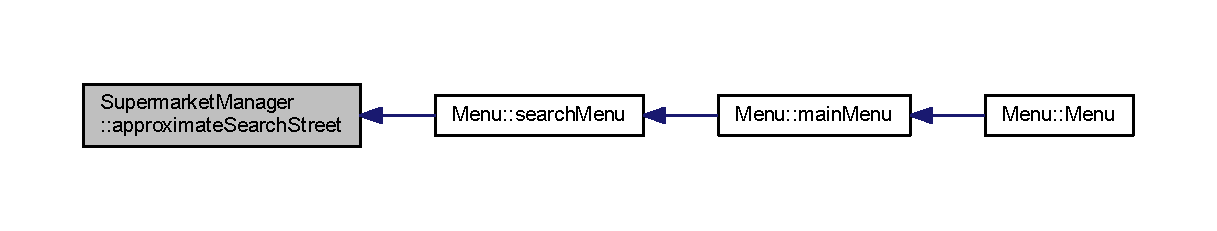
\includegraphics[width=350pt]{class_supermarket_manager_a0aa3fa8dab27db5f4960b840a2dd871c_icgraph}
\end{center}
\end{figure}
\mbox{\Hypertarget{class_supermarket_manager_af797d69ada273a0582a619a0fc8f0638}\label{class_supermarket_manager_af797d69ada273a0582a619a0fc8f0638}} 
\index{Supermarket\+Manager@{Supermarket\+Manager}!approximate\+Search\+Supermarket@{approximate\+Search\+Supermarket}}
\index{approximate\+Search\+Supermarket@{approximate\+Search\+Supermarket}!Supermarket\+Manager@{Supermarket\+Manager}}
\subsubsection{\texorpdfstring{approximate\+Search\+Supermarket()}{approximateSearchSupermarket()}}
{\footnotesize\ttfamily void Supermarket\+Manager\+::approximate\+Search\+Supermarket (\begin{DoxyParamCaption}{ }\end{DoxyParamCaption})}

Realiza a pesquisa aproximada de cadeias de supermercados Here is the caller graph for this function\+:
\nopagebreak
\begin{figure}[H]
\begin{center}
\leavevmode
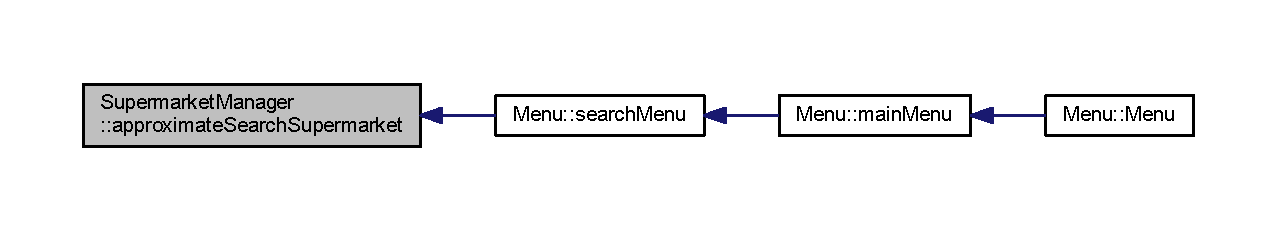
\includegraphics[width=350pt]{class_supermarket_manager_af797d69ada273a0582a619a0fc8f0638_icgraph}
\end{center}
\end{figure}
\mbox{\Hypertarget{class_supermarket_manager_a7eca833133baf500e2a63b2ec9746b1d}\label{class_supermarket_manager_a7eca833133baf500e2a63b2ec9746b1d}} 
\index{Supermarket\+Manager@{Supermarket\+Manager}!check\+Street@{check\+Street}}
\index{check\+Street@{check\+Street}!Supermarket\+Manager@{Supermarket\+Manager}}
\subsubsection{\texorpdfstring{check\+Street()}{checkStreet()}}
{\footnotesize\ttfamily void Supermarket\+Manager\+::check\+Street (\begin{DoxyParamCaption}\item[{\hyperlink{class_node_object}{Node\+Object} $\ast$}]{market }\end{DoxyParamCaption})}

Imprime o nome da(s) rua(s) em que o supermercado se encontra 
\begin{DoxyParams}{Parameters}
{\em market} & supermercado a pesquisar \\
\hline
\end{DoxyParams}
\mbox{\Hypertarget{class_supermarket_manager_a23d192df8b8a56e317632845f9bb81d6}\label{class_supermarket_manager_a23d192df8b8a56e317632845f9bb81d6}} 
\index{Supermarket\+Manager@{Supermarket\+Manager}!check\+Supermarket\+Existence@{check\+Supermarket\+Existence}}
\index{check\+Supermarket\+Existence@{check\+Supermarket\+Existence}!Supermarket\+Manager@{Supermarket\+Manager}}
\subsubsection{\texorpdfstring{check\+Supermarket\+Existence()}{checkSupermarketExistence()}}
{\footnotesize\ttfamily void Supermarket\+Manager\+::check\+Supermarket\+Existence (\begin{DoxyParamCaption}\item[{\hyperlink{class_edge}{Edge}$<$ \hyperlink{class_node_object}{Node\+Object} $\ast$$>$}]{e }\end{DoxyParamCaption})}

Imprime as informacoes dos supermercados, se existirem, que se encontram na rua 
\begin{DoxyParams}{Parameters}
{\em e} & rua a pesquisar \\
\hline
\end{DoxyParams}
Here is the call graph for this function\+:
\nopagebreak
\begin{figure}[H]
\begin{center}
\leavevmode
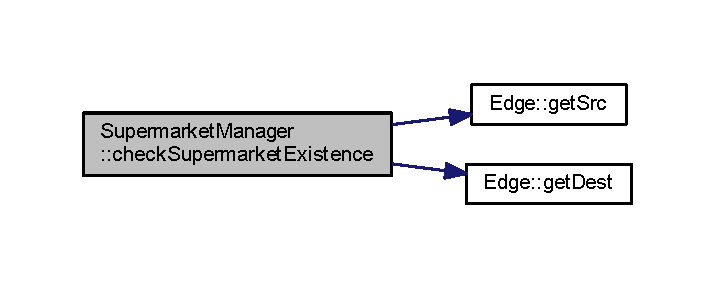
\includegraphics[width=343pt]{class_supermarket_manager_a23d192df8b8a56e317632845f9bb81d6_cgraph}
\end{center}
\end{figure}
\mbox{\Hypertarget{class_supermarket_manager_a034d77cc6da77516f6dbb4d6c3c0513d}\label{class_supermarket_manager_a034d77cc6da77516f6dbb4d6c3c0513d}} 
\index{Supermarket\+Manager@{Supermarket\+Manager}!deliver\+All\+Requests@{deliver\+All\+Requests}}
\index{deliver\+All\+Requests@{deliver\+All\+Requests}!Supermarket\+Manager@{Supermarket\+Manager}}
\subsubsection{\texorpdfstring{deliver\+All\+Requests()}{deliverAllRequests()}}
{\footnotesize\ttfamily void Supermarket\+Manager\+::deliver\+All\+Requests (\begin{DoxyParamCaption}\item[{int}]{choice }\end{DoxyParamCaption})}

Esta fun��o entrega os pedidos pendentes de todos os supermercados. A abordagem utilizada depender� do parametro \textquotesingle{}choice\textquotesingle{}. Ver fun��o \textquotesingle{}deliver\+Requests\textquotesingle{} da classe \hyperlink{class_supermercado}{Supermercado}.


\begin{DoxyParams}{Parameters}
{\em choice} & inteiro que determina a estrat�gia utilizada na entrega dos pedidos \\
\hline
\end{DoxyParams}
Here is the caller graph for this function\+:
\nopagebreak
\begin{figure}[H]
\begin{center}
\leavevmode
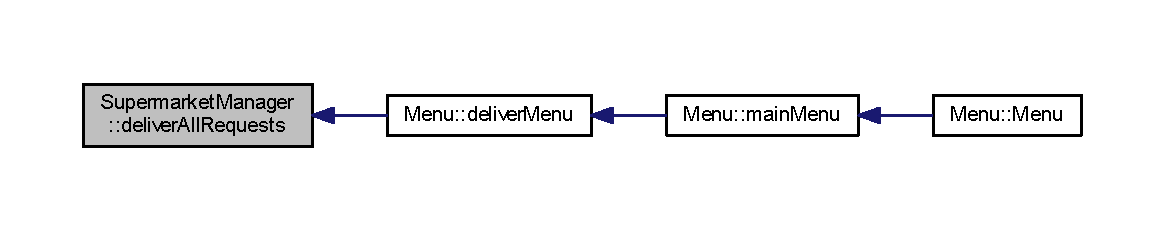
\includegraphics[width=350pt]{class_supermarket_manager_a034d77cc6da77516f6dbb4d6c3c0513d_icgraph}
\end{center}
\end{figure}
\mbox{\Hypertarget{class_supermarket_manager_a16c8f9e3da09e91cb50d0ae932bb4eb2}\label{class_supermarket_manager_a16c8f9e3da09e91cb50d0ae932bb4eb2}} 
\index{Supermarket\+Manager@{Supermarket\+Manager}!edit\+Distance@{edit\+Distance}}
\index{edit\+Distance@{edit\+Distance}!Supermarket\+Manager@{Supermarket\+Manager}}
\subsubsection{\texorpdfstring{edit\+Distance()}{editDistance()}}
{\footnotesize\ttfamily int Supermarket\+Manager\+::edit\+Distance (\begin{DoxyParamCaption}\item[{string}]{T,  }\item[{string}]{P }\end{DoxyParamCaption})}

Retorna a distancia entre duas strings 
\begin{DoxyParams}{Parameters}
{\em T} & string onde a comparacao ocorre \\
\hline
{\em P} & string onde a comparacao ocorre \\
\hline
\end{DoxyParams}
\begin{DoxyReturn}{Returns}
distancia entre as strings 
\end{DoxyReturn}
\mbox{\Hypertarget{class_supermarket_manager_addbb66cfbe7d097687595c38e16b9c62}\label{class_supermarket_manager_addbb66cfbe7d097687595c38e16b9c62}} 
\index{Supermarket\+Manager@{Supermarket\+Manager}!exact\+Search\+District@{exact\+Search\+District}}
\index{exact\+Search\+District@{exact\+Search\+District}!Supermarket\+Manager@{Supermarket\+Manager}}
\subsubsection{\texorpdfstring{exact\+Search\+District()}{exactSearchDistrict()}}
{\footnotesize\ttfamily void Supermarket\+Manager\+::exact\+Search\+District (\begin{DoxyParamCaption}{ }\end{DoxyParamCaption})}

Realiza a pesquisa exacta de ruas Here is the caller graph for this function\+:
\nopagebreak
\begin{figure}[H]
\begin{center}
\leavevmode
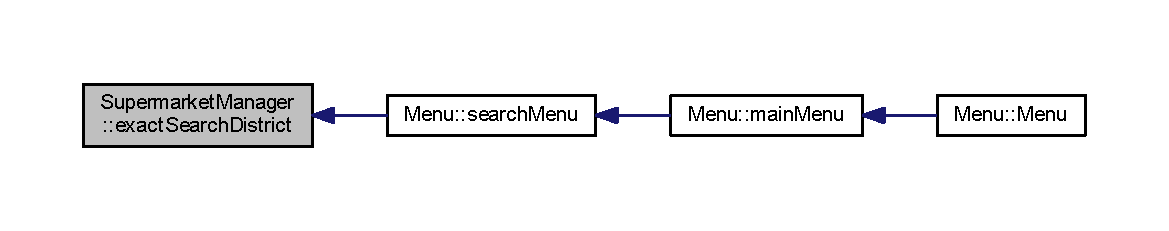
\includegraphics[width=350pt]{class_supermarket_manager_addbb66cfbe7d097687595c38e16b9c62_icgraph}
\end{center}
\end{figure}
\mbox{\Hypertarget{class_supermarket_manager_a7fa00d7adf078ca864908c901371a60c}\label{class_supermarket_manager_a7fa00d7adf078ca864908c901371a60c}} 
\index{Supermarket\+Manager@{Supermarket\+Manager}!exact\+Search\+Street@{exact\+Search\+Street}}
\index{exact\+Search\+Street@{exact\+Search\+Street}!Supermarket\+Manager@{Supermarket\+Manager}}
\subsubsection{\texorpdfstring{exact\+Search\+Street()}{exactSearchStreet()}}
{\footnotesize\ttfamily void Supermarket\+Manager\+::exact\+Search\+Street (\begin{DoxyParamCaption}{ }\end{DoxyParamCaption})}

Realiza a pesquisa exacta de ruas Here is the caller graph for this function\+:
\nopagebreak
\begin{figure}[H]
\begin{center}
\leavevmode
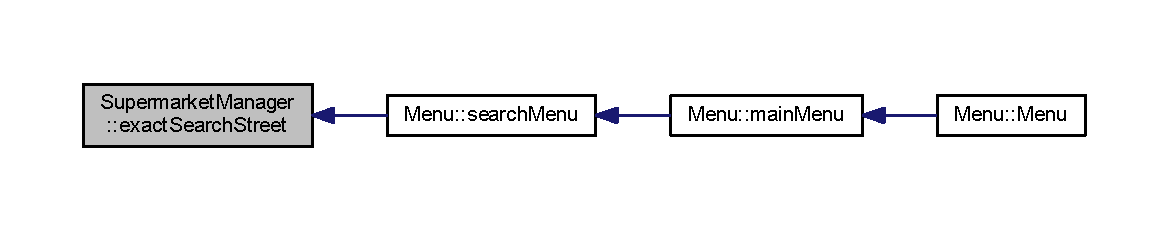
\includegraphics[width=350pt]{class_supermarket_manager_a7fa00d7adf078ca864908c901371a60c_icgraph}
\end{center}
\end{figure}
\mbox{\Hypertarget{class_supermarket_manager_a9841cd0c676abc1f128a68bb71bc2683}\label{class_supermarket_manager_a9841cd0c676abc1f128a68bb71bc2683}} 
\index{Supermarket\+Manager@{Supermarket\+Manager}!exact\+Search\+Supermarket@{exact\+Search\+Supermarket}}
\index{exact\+Search\+Supermarket@{exact\+Search\+Supermarket}!Supermarket\+Manager@{Supermarket\+Manager}}
\subsubsection{\texorpdfstring{exact\+Search\+Supermarket()}{exactSearchSupermarket()}}
{\footnotesize\ttfamily void Supermarket\+Manager\+::exact\+Search\+Supermarket (\begin{DoxyParamCaption}{ }\end{DoxyParamCaption})}

Realiza a pesquisa exacta de cadeias de supermercados Here is the caller graph for this function\+:
\nopagebreak
\begin{figure}[H]
\begin{center}
\leavevmode
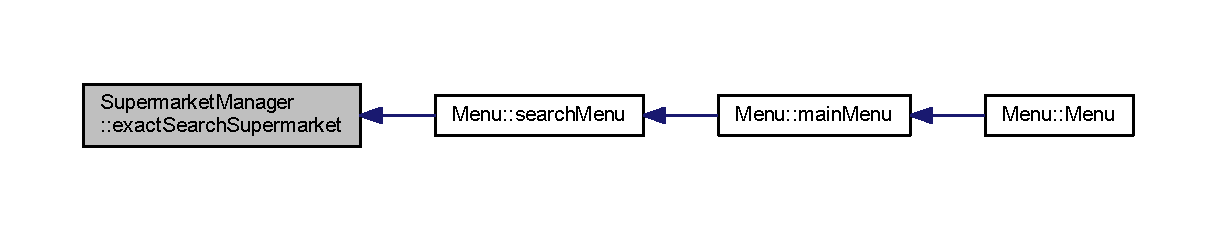
\includegraphics[width=350pt]{class_supermarket_manager_a9841cd0c676abc1f128a68bb71bc2683_icgraph}
\end{center}
\end{figure}
\mbox{\Hypertarget{class_supermarket_manager_a3869489967f0a60d1b9c36a85b05998b}\label{class_supermarket_manager_a3869489967f0a60d1b9c36a85b05998b}} 
\index{Supermarket\+Manager@{Supermarket\+Manager}!find\+Nearest\+Supermarket@{find\+Nearest\+Supermarket}}
\index{find\+Nearest\+Supermarket@{find\+Nearest\+Supermarket}!Supermarket\+Manager@{Supermarket\+Manager}}
\subsubsection{\texorpdfstring{find\+Nearest\+Supermarket()}{findNearestSupermarket()}}
{\footnotesize\ttfamily \hyperlink{class_supermercado}{Supermercado} $\ast$ Supermarket\+Manager\+::find\+Nearest\+Supermarket (\begin{DoxyParamCaption}\item[{\hyperlink{class_client}{Client} $\ast$}]{client }\end{DoxyParamCaption})}

Retorna o supermercado mais proximo do cliente dado. Caso nenhum supermercado desta cadeia tenha um caminho at� ao cliente, a fun��o retorna \textquotesingle{}nullptr\textquotesingle{}.

\begin{DoxyReturn}{Returns}
o supermercado mais proximo do cliente dado 
\end{DoxyReturn}
Here is the call graph for this function\+:
\nopagebreak
\begin{figure}[H]
\begin{center}
\leavevmode
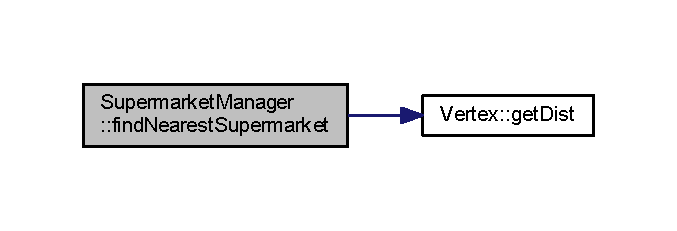
\includegraphics[width=325pt]{class_supermarket_manager_a3869489967f0a60d1b9c36a85b05998b_cgraph}
\end{center}
\end{figure}
\mbox{\Hypertarget{class_supermarket_manager_a15c50e904600847775367ff4f626f62d}\label{class_supermarket_manager_a15c50e904600847775367ff4f626f62d}} 
\index{Supermarket\+Manager@{Supermarket\+Manager}!get\+Client@{get\+Client}}
\index{get\+Client@{get\+Client}!Supermarket\+Manager@{Supermarket\+Manager}}
\subsubsection{\texorpdfstring{get\+Client()}{getClient()}}
{\footnotesize\ttfamily \hyperlink{class_client}{Client} $\ast$ Supermarket\+Manager\+::get\+Client (\begin{DoxyParamCaption}\item[{int}]{id }\end{DoxyParamCaption})}

Retorna um apontador para o cliente de ID dado.


\begin{DoxyParams}{Parameters}
{\em id} & ID do cliente \\
\hline
\end{DoxyParams}
\begin{DoxyReturn}{Returns}
um apontador para o cliente de ID dado 
\end{DoxyReturn}
\mbox{\Hypertarget{class_supermarket_manager_a45ed55914bea37bcf0d5757d1ce027c4}\label{class_supermarket_manager_a45ed55914bea37bcf0d5757d1ce027c4}} 
\index{Supermarket\+Manager@{Supermarket\+Manager}!input\+Client\+ID@{input\+Client\+ID}}
\index{input\+Client\+ID@{input\+Client\+ID}!Supermarket\+Manager@{Supermarket\+Manager}}
\subsubsection{\texorpdfstring{input\+Client\+I\+D()}{inputClientID()}}
{\footnotesize\ttfamily int Supermarket\+Manager\+::input\+Client\+ID (\begin{DoxyParamCaption}{ }\end{DoxyParamCaption})}

Pede continuamente ao utilizador o ID de um cliente at� que este corresponda ao ID de um cliente que exista no vetor client\+List. Retorna esse ID, garantidamente v�lido.

\begin{DoxyReturn}{Returns}
ID do cliente validado 
\end{DoxyReturn}
Here is the call graph for this function\+:
\nopagebreak
\begin{figure}[H]
\begin{center}
\leavevmode
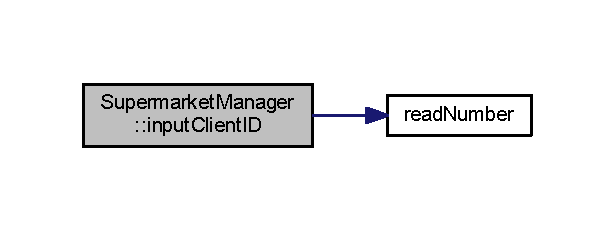
\includegraphics[width=295pt]{class_supermarket_manager_a45ed55914bea37bcf0d5757d1ce027c4_cgraph}
\end{center}
\end{figure}
\mbox{\Hypertarget{class_supermarket_manager_a6a688cb8cec4cc323cf4e53e04068c2c}\label{class_supermarket_manager_a6a688cb8cec4cc323cf4e53e04068c2c}} 
\index{Supermarket\+Manager@{Supermarket\+Manager}!kmp\+Matcher@{kmp\+Matcher}}
\index{kmp\+Matcher@{kmp\+Matcher}!Supermarket\+Manager@{Supermarket\+Manager}}
\subsubsection{\texorpdfstring{kmp\+Matcher()}{kmpMatcher()}}
{\footnotesize\ttfamily bool Supermarket\+Manager\+::kmp\+Matcher (\begin{DoxyParamCaption}\item[{string}]{T,  }\item[{string}]{P }\end{DoxyParamCaption})}

Pesquisa de string exata 
\begin{DoxyParams}{Parameters}
{\em T} & string onde ocorre a pesquisa \\
\hline
{\em P} & string a ser pesquisada \\
\hline
\end{DoxyParams}
\begin{DoxyReturn}{Returns}
retorna true se P ocorre em T, false caso contrario 
\end{DoxyReturn}
\mbox{\Hypertarget{class_supermarket_manager_a0072988df7db4459fe0a409894af51a4}\label{class_supermarket_manager_a0072988df7db4459fe0a409894af51a4}} 
\index{Supermarket\+Manager@{Supermarket\+Manager}!load\+Graph@{load\+Graph}}
\index{load\+Graph@{load\+Graph}!Supermarket\+Manager@{Supermarket\+Manager}}
\subsubsection{\texorpdfstring{load\+Graph()}{loadGraph()}}
{\footnotesize\ttfamily void Supermarket\+Manager\+::load\+Graph (\begin{DoxyParamCaption}{ }\end{DoxyParamCaption})}

Le de um ficheiro as informacoes necessarias para preencher o vetores client\+List e market\+List, adicionar os respetivos nos ao grafo e ainda as suas arestas. Here is the call graph for this function\+:
\nopagebreak
\begin{figure}[H]
\begin{center}
\leavevmode
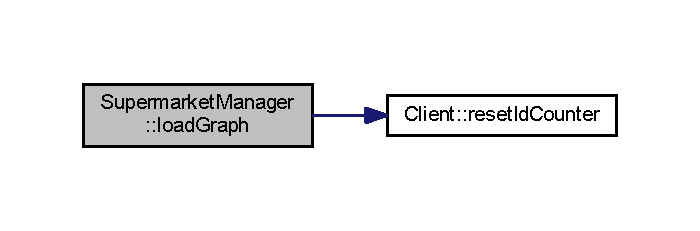
\includegraphics[width=336pt]{class_supermarket_manager_a0072988df7db4459fe0a409894af51a4_cgraph}
\end{center}
\end{figure}
Here is the caller graph for this function\+:
\nopagebreak
\begin{figure}[H]
\begin{center}
\leavevmode
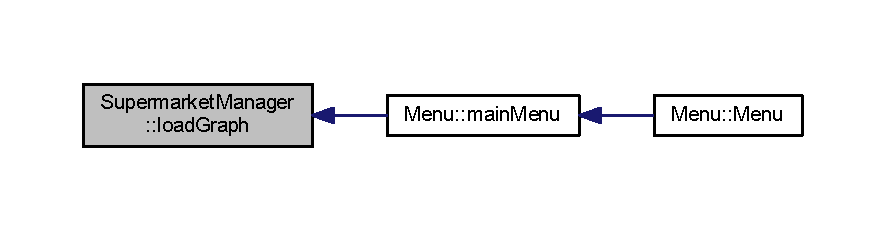
\includegraphics[width=350pt]{class_supermarket_manager_a0072988df7db4459fe0a409894af51a4_icgraph}
\end{center}
\end{figure}
\mbox{\Hypertarget{class_supermarket_manager_abab275f63e6169a76efd92c90aaac0b4}\label{class_supermarket_manager_abab275f63e6169a76efd92c90aaac0b4}} 
\index{Supermarket\+Manager@{Supermarket\+Manager}!make\+Graph@{make\+Graph}}
\index{make\+Graph@{make\+Graph}!Supermarket\+Manager@{Supermarket\+Manager}}
\subsubsection{\texorpdfstring{make\+Graph()}{makeGraph()}}
{\footnotesize\ttfamily void Supermarket\+Manager\+::make\+Graph (\begin{DoxyParamCaption}{ }\end{DoxyParamCaption})}

Cria um grafo com um numero de clientes, supermercados e arestas introduzidos pelo utilizador. Here is the call graph for this function\+:
\nopagebreak
\begin{figure}[H]
\begin{center}
\leavevmode
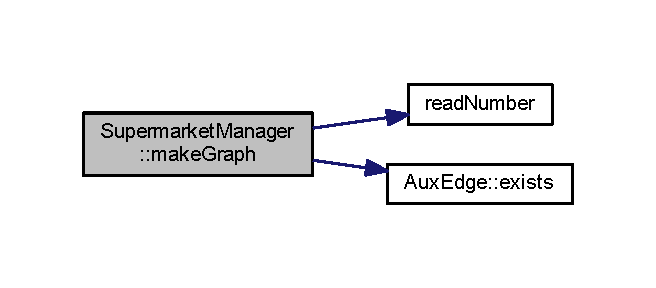
\includegraphics[width=315pt]{class_supermarket_manager_abab275f63e6169a76efd92c90aaac0b4_cgraph}
\end{center}
\end{figure}
Here is the caller graph for this function\+:
\nopagebreak
\begin{figure}[H]
\begin{center}
\leavevmode
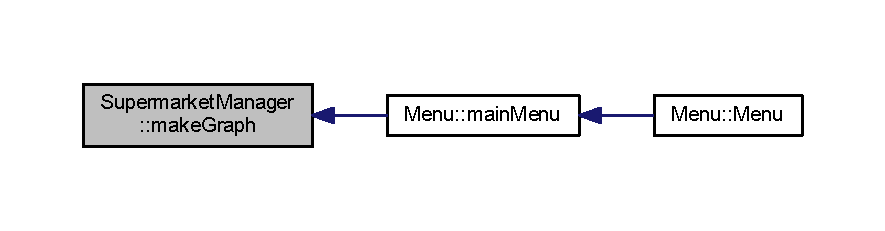
\includegraphics[width=350pt]{class_supermarket_manager_abab275f63e6169a76efd92c90aaac0b4_icgraph}
\end{center}
\end{figure}
\mbox{\Hypertarget{class_supermarket_manager_a6dbf83eef3433341c7a971860e3b8915}\label{class_supermarket_manager_a6dbf83eef3433341c7a971860e3b8915}} 
\index{Supermarket\+Manager@{Supermarket\+Manager}!make\+Random\+Requests@{make\+Random\+Requests}}
\index{make\+Random\+Requests@{make\+Random\+Requests}!Supermarket\+Manager@{Supermarket\+Manager}}
\subsubsection{\texorpdfstring{make\+Random\+Requests()}{makeRandomRequests()}}
{\footnotesize\ttfamily void Supermarket\+Manager\+::make\+Random\+Requests (\begin{DoxyParamCaption}{ }\end{DoxyParamCaption})}

Atribui um pedido de tamanho aletorio a todos os clientes. Here is the call graph for this function\+:
\nopagebreak
\begin{figure}[H]
\begin{center}
\leavevmode
\includegraphics[width=350pt]{class_supermarket_manager_a6dbf83eef3433341c7a971860e3b8915_cgraph}
\end{center}
\end{figure}
Here is the caller graph for this function\+:
\nopagebreak
\begin{figure}[H]
\begin{center}
\leavevmode
\includegraphics[width=350pt]{class_supermarket_manager_a6dbf83eef3433341c7a971860e3b8915_icgraph}
\end{center}
\end{figure}
\mbox{\Hypertarget{class_supermarket_manager_a19901c8d338b7579398373aeda62ecf2}\label{class_supermarket_manager_a19901c8d338b7579398373aeda62ecf2}} 
\index{Supermarket\+Manager@{Supermarket\+Manager}!make\+Request@{make\+Request}}
\index{make\+Request@{make\+Request}!Supermarket\+Manager@{Supermarket\+Manager}}
\subsubsection{\texorpdfstring{make\+Request()}{makeRequest()}}
{\footnotesize\ttfamily void Supermarket\+Manager\+::make\+Request (\begin{DoxyParamCaption}{ }\end{DoxyParamCaption})}

Pede ao utilizador o ID do cliente e o tamanho do pedido que este cliente pretende efetuar. Em seguida, encontra o supermercado mais pr�ximo do cliente, adicionando o pedido � fila de prioridade de pedidos desse supermercado. Caso nenhum supermercado desta cadeia tenha um caminho at� ao cliente, a fun��o mostra uma mensagem de erro e retorna. Here is the call graph for this function\+:
\nopagebreak
\begin{figure}[H]
\begin{center}
\leavevmode
\includegraphics[width=350pt]{class_supermarket_manager_a19901c8d338b7579398373aeda62ecf2_cgraph}
\end{center}
\end{figure}
Here is the caller graph for this function\+:
\nopagebreak
\begin{figure}[H]
\begin{center}
\leavevmode
\includegraphics[width=350pt]{class_supermarket_manager_a19901c8d338b7579398373aeda62ecf2_icgraph}
\end{center}
\end{figure}
\mbox{\Hypertarget{class_supermarket_manager_a882d9161a59b259f5b0f62c230c11db9}\label{class_supermarket_manager_a882d9161a59b259f5b0f62c230c11db9}} 
\index{Supermarket\+Manager@{Supermarket\+Manager}!populate\+Graph@{populate\+Graph}}
\index{populate\+Graph@{populate\+Graph}!Supermarket\+Manager@{Supermarket\+Manager}}
\subsubsection{\texorpdfstring{populate\+Graph()}{populateGraph()}}
{\footnotesize\ttfamily void Supermarket\+Manager\+::populate\+Graph (\begin{DoxyParamCaption}{ }\end{DoxyParamCaption})}

Adiciona ao grafo os v�rtices correspondentes aos clientes e supermercados dos vetores client\+List e market\+List \mbox{\Hypertarget{class_supermarket_manager_a3f18b0466fcb9369084ecd0c4e2d2e4a}\label{class_supermarket_manager_a3f18b0466fcb9369084ecd0c4e2d2e4a}} 
\index{Supermarket\+Manager@{Supermarket\+Manager}!prefix\+Computation@{prefix\+Computation}}
\index{prefix\+Computation@{prefix\+Computation}!Supermarket\+Manager@{Supermarket\+Manager}}
\subsubsection{\texorpdfstring{prefix\+Computation()}{prefixComputation()}}
{\footnotesize\ttfamily vector$<$ int $>$ Supermarket\+Manager\+::prefix\+Computation (\begin{DoxyParamCaption}\item[{string}]{P }\end{DoxyParamCaption})}

Realiza o preprocessamento da string a ser pesquisada na funcao kmp\+Matcher 
\begin{DoxyParams}{Parameters}
{\em P} & string a ser preprocessada \\
\hline
\end{DoxyParams}
\begin{DoxyReturn}{Returns}
retorna um vetor com o resultado do preprocessamento da string 
\end{DoxyReturn}
\mbox{\Hypertarget{class_supermarket_manager_a3bbfc2db4c66bbaab3a5536c7205a818}\label{class_supermarket_manager_a3bbfc2db4c66bbaab3a5536c7205a818}} 
\index{Supermarket\+Manager@{Supermarket\+Manager}!show\+Info@{show\+Info}}
\index{show\+Info@{show\+Info}!Supermarket\+Manager@{Supermarket\+Manager}}
\subsubsection{\texorpdfstring{show\+Info()}{showInfo()}}
{\footnotesize\ttfamily void Supermarket\+Manager\+::show\+Info (\begin{DoxyParamCaption}{ }\end{DoxyParamCaption})}

Imprime algumas informa��es tais como o n�mero de clientes e de supermercados desta cadeia de supermercados. Efetua uma an�lise da densidade e conetividade do grafo e mostra ainda as suas componentes fortemente conexas. Here is the call graph for this function\+:
\nopagebreak
\begin{figure}[H]
\begin{center}
\leavevmode
\includegraphics[width=312pt]{class_supermarket_manager_a3bbfc2db4c66bbaab3a5536c7205a818_cgraph}
\end{center}
\end{figure}
\mbox{\Hypertarget{class_supermarket_manager_a325c08bab73c6ddfe61dbb600c8d55fd}\label{class_supermarket_manager_a325c08bab73c6ddfe61dbb600c8d55fd}} 
\index{Supermarket\+Manager@{Supermarket\+Manager}!strongly\+Connected\+Components@{strongly\+Connected\+Components}}
\index{strongly\+Connected\+Components@{strongly\+Connected\+Components}!Supermarket\+Manager@{Supermarket\+Manager}}
\subsubsection{\texorpdfstring{strongly\+Connected\+Components()}{stronglyConnectedComponents()}}
{\footnotesize\ttfamily void Supermarket\+Manager\+::strongly\+Connected\+Components (\begin{DoxyParamCaption}{ }\end{DoxyParamCaption})}

Imprime as componentes fortemente conexas do grafo. Here is the call graph for this function\+:
\nopagebreak
\begin{figure}[H]
\begin{center}
\leavevmode
\includegraphics[width=350pt]{class_supermarket_manager_a325c08bab73c6ddfe61dbb600c8d55fd_cgraph}
\end{center}
\end{figure}


\subsection{Member Data Documentation}
\mbox{\Hypertarget{class_supermarket_manager_a48c5227a7d0ca5f8db9de726184e116a}\label{class_supermarket_manager_a48c5227a7d0ca5f8db9de726184e116a}} 
\index{Supermarket\+Manager@{Supermarket\+Manager}!client\+List@{client\+List}}
\index{client\+List@{client\+List}!Supermarket\+Manager@{Supermarket\+Manager}}
\subsubsection{\texorpdfstring{client\+List}{clientList}}
{\footnotesize\ttfamily vector$<$\hyperlink{class_client}{Client}$\ast$$>$ Supermarket\+Manager\+::client\+List\hspace{0.3cm}{\ttfamily [private]}}

Vetor de apontadores para os clientes desta cadeia de supermercados. \mbox{\Hypertarget{class_supermarket_manager_ab2cc638ffffc81beda833ca864e8bd62}\label{class_supermarket_manager_ab2cc638ffffc81beda833ca864e8bd62}} 
\index{Supermarket\+Manager@{Supermarket\+Manager}!graph@{graph}}
\index{graph@{graph}!Supermarket\+Manager@{Supermarket\+Manager}}
\subsubsection{\texorpdfstring{graph}{graph}}
{\footnotesize\ttfamily \hyperlink{class_graph}{Graph}$<$\hyperlink{class_node_object}{Node\+Object}$\ast$$>$ Supermarket\+Manager\+::graph\hspace{0.3cm}{\ttfamily [private]}}

Grafo de n�s correspondestes aos clientes e supermercados. \mbox{\Hypertarget{class_supermarket_manager_a122812406afbf7d0d130d39e6921d5f5}\label{class_supermarket_manager_a122812406afbf7d0d130d39e6921d5f5}} 
\index{Supermarket\+Manager@{Supermarket\+Manager}!market\+List@{market\+List}}
\index{market\+List@{market\+List}!Supermarket\+Manager@{Supermarket\+Manager}}
\subsubsection{\texorpdfstring{market\+List}{marketList}}
{\footnotesize\ttfamily vector$<$\hyperlink{class_supermercado}{Supermercado}$\ast$$>$ Supermarket\+Manager\+::market\+List\hspace{0.3cm}{\ttfamily [private]}}

Vetor de apontadores para os supermercados desta cadeia de supermercados. 

The documentation for this class was generated from the following files\+:\begin{DoxyCompactItemize}
\item 
\hyperlink{_supermarket_manager_8h}{Supermarket\+Manager.\+h}\item 
\hyperlink{_supermarket_manager_8cpp}{Supermarket\+Manager.\+cpp}\end{DoxyCompactItemize}

\hypertarget{class_supermercado}{}\section{Supermercado Class Reference}
\label{class_supermercado}\index{Supermercado@{Supermercado}}


{\ttfamily \#include $<$Supermercado.\+h$>$}



Inheritance diagram for Supermercado\+:
\nopagebreak
\begin{figure}[H]
\begin{center}
\leavevmode
\includegraphics[width=160pt]{class_supermercado__inherit__graph}
\end{center}
\end{figure}


Collaboration diagram for Supermercado\+:
\nopagebreak
\begin{figure}[H]
\begin{center}
\leavevmode
\includegraphics[width=160pt]{class_supermercado__coll__graph}
\end{center}
\end{figure}
\subsection*{Public Member Functions}
\begin{DoxyCompactItemize}
\item 
\hyperlink{class_supermercado_abb04a5d0aa1f9c2550c1f3e48da26d5a}{Supermercado} (int nr\+Trucks, string cadeia)
\item 
void \hyperlink{class_supermercado_a314239f694ade17210e7d50689f49fc5}{add\+Request} (\hyperlink{class_pedido}{Pedido} $\ast$request)
\item 
int \hyperlink{class_supermercado_af5f0635dbc5b61a185c74f37f4ee1f92}{get\+Request\+Number} ()
\item 
void \hyperlink{class_supermercado_ad24337eae5c068802738319ec4331772}{deliver\+Requests} (\hyperlink{class_graph}{Graph}$<$ \hyperlink{class_node_object}{Node\+Object} $\ast$$>$ graph, int choice)
\item 
void \hyperlink{class_supermercado_aa7ec7166a13ba5839aec12ff65b599aa}{fill\+Trucks\+Size} (\hyperlink{class_graph}{Graph}$<$ \hyperlink{class_node_object}{Node\+Object} $\ast$$>$ graph)
\item 
void \hyperlink{class_supermercado_afaaae4505e9900f6f44800118280aafb}{fill\+Trucks\+Distance} (\hyperlink{class_graph}{Graph}$<$ \hyperlink{class_node_object}{Node\+Object} $\ast$$>$ graph)
\item 
int \hyperlink{class_supermercado_abcbce3640cbb395c1b9cd3bd07b11316}{get\+Number\+Trucks} ()
\item 
string \hyperlink{class_supermercado_a43b014953172f2e6aa09003da36a5194}{get\+Cadeia\+Supermercado} ()
\end{DoxyCompactItemize}
\subsection*{Private Attributes}
\begin{DoxyCompactItemize}
\item 
priority\+\_\+queue$<$ \hyperlink{class_pedido}{Pedido} $\ast$, vector$<$ \hyperlink{class_pedido}{Pedido} $\ast$ $>$, \hyperlink{class_comparison_request_size}{Comparison\+Request\+Size} $>$ \hyperlink{class_supermercado_a0f8759dc0543f6902264f9f9e7d436a0}{pedidos}
\item 
vector$<$ \hyperlink{class_camiao}{Camiao} $\ast$ $>$ \hyperlink{class_supermercado_a680cc129a590b0b87f2cb4dc200f9901}{camioes}
\item 
string \hyperlink{class_supermercado_a9f26a07c7740187fd52f6d9e56452cad}{cadeia\+Supermercado}
\end{DoxyCompactItemize}
\subsection*{Additional Inherited Members}


\subsection{Constructor \& Destructor Documentation}
\mbox{\Hypertarget{class_supermercado_abb04a5d0aa1f9c2550c1f3e48da26d5a}\label{class_supermercado_abb04a5d0aa1f9c2550c1f3e48da26d5a}} 
\index{Supermercado@{Supermercado}!Supermercado@{Supermercado}}
\index{Supermercado@{Supermercado}!Supermercado@{Supermercado}}
\subsubsection{\texorpdfstring{Supermercado()}{Supermercado()}}
{\footnotesize\ttfamily Supermercado\+::\+Supermercado (\begin{DoxyParamCaption}\item[{int}]{nr\+Trucks,  }\item[{string}]{cadeia }\end{DoxyParamCaption})}

Contrutor do supermercado. O n�mero de cami�es que o supermercado possuir� � igual \textquotesingle{}nr\+Trucks\textquotesingle{}.


\begin{DoxyParams}{Parameters}
{\em nr\+Trucks} & n�mero de cami�es que o supermercado possuir� \\
\hline
{\em cadeia} & cadeia a que o supermercado pertence \\
\hline
\end{DoxyParams}


\subsection{Member Function Documentation}
\mbox{\Hypertarget{class_supermercado_a314239f694ade17210e7d50689f49fc5}\label{class_supermercado_a314239f694ade17210e7d50689f49fc5}} 
\index{Supermercado@{Supermercado}!add\+Request@{add\+Request}}
\index{add\+Request@{add\+Request}!Supermercado@{Supermercado}}
\subsubsection{\texorpdfstring{add\+Request()}{addRequest()}}
{\footnotesize\ttfamily void Supermercado\+::add\+Request (\begin{DoxyParamCaption}\item[{\hyperlink{class_pedido}{Pedido} $\ast$}]{request }\end{DoxyParamCaption})}

Adiciona um apontador para um pedido � fila de prioridade pedidos, tendo em conta que adicionar v�rios pedidos de um mesmo cliente apenas atualiza o tamanho do pedido desse cliente, n�o criando novas inst�ncias na fila de prioridade.


\begin{DoxyParams}{Parameters}
{\em request} & pedido a adicionar � fila de prioridade \textquotesingle{}pedidos\textquotesingle{} \\
\hline
\end{DoxyParams}
Here is the call graph for this function\+:
\nopagebreak
\begin{figure}[H]
\begin{center}
\leavevmode
\includegraphics[width=350pt]{class_supermercado_a314239f694ade17210e7d50689f49fc5_cgraph}
\end{center}
\end{figure}
Here is the caller graph for this function\+:
\nopagebreak
\begin{figure}[H]
\begin{center}
\leavevmode
\includegraphics[width=350pt]{class_supermercado_a314239f694ade17210e7d50689f49fc5_icgraph}
\end{center}
\end{figure}
\mbox{\Hypertarget{class_supermercado_ad24337eae5c068802738319ec4331772}\label{class_supermercado_ad24337eae5c068802738319ec4331772}} 
\index{Supermercado@{Supermercado}!deliver\+Requests@{deliver\+Requests}}
\index{deliver\+Requests@{deliver\+Requests}!Supermercado@{Supermercado}}
\subsubsection{\texorpdfstring{deliver\+Requests()}{deliverRequests()}}
{\footnotesize\ttfamily void Supermercado\+::deliver\+Requests (\begin{DoxyParamCaption}\item[{\hyperlink{class_graph}{Graph}$<$ \hyperlink{class_node_object}{Node\+Object} $\ast$$>$}]{graph,  }\item[{int}]{choice }\end{DoxyParamCaption})}

Entrega aos clientes deste supermercado todos os seus pedidos pendentes. Caso \textquotesingle{}choice\textquotesingle{} seja 0 pretende-\/se que os cami�es tranportem o m�ximo de pedidos numa s� viagem. Caso \textquotesingle{}choice\textquotesingle{} seja 1 o objectivo ser� que os cami�es percorram uma dist�ncia total m�nima ao entregar os pedidos.


\begin{DoxyParams}{Parameters}
{\em graph} & grafo da cadeia de supermercados considerada \\
\hline
{\em choice} & inteiro que determina a estrat�gia utilizada na entrega dos pedidos \\
\hline
\end{DoxyParams}
Here is the call graph for this function\+:
\nopagebreak
\begin{figure}[H]
\begin{center}
\leavevmode
\includegraphics[width=350pt]{class_supermercado_ad24337eae5c068802738319ec4331772_cgraph}
\end{center}
\end{figure}
\mbox{\Hypertarget{class_supermercado_afaaae4505e9900f6f44800118280aafb}\label{class_supermercado_afaaae4505e9900f6f44800118280aafb}} 
\index{Supermercado@{Supermercado}!fill\+Trucks\+Distance@{fill\+Trucks\+Distance}}
\index{fill\+Trucks\+Distance@{fill\+Trucks\+Distance}!Supermercado@{Supermercado}}
\subsubsection{\texorpdfstring{fill\+Trucks\+Distance()}{fillTrucksDistance()}}
{\footnotesize\ttfamily void Supermercado\+::fill\+Trucks\+Distance (\begin{DoxyParamCaption}\item[{\hyperlink{class_graph}{Graph}$<$ \hyperlink{class_node_object}{Node\+Object} $\ast$$>$}]{graph }\end{DoxyParamCaption})}

Distribui os pedidos pelos cami�es, determinando seu itener�rio de modo a que cada cami�o percorra uma dist�ncia total m�nima ao entregar os pedidos.


\begin{DoxyParams}{Parameters}
{\em graph} & grafo da cadeia de supermercados considerada \\
\hline
\end{DoxyParams}
Here is the call graph for this function\+:
\nopagebreak
\begin{figure}[H]
\begin{center}
\leavevmode
\includegraphics[width=350pt]{class_supermercado_afaaae4505e9900f6f44800118280aafb_cgraph}
\end{center}
\end{figure}
Here is the caller graph for this function\+:
\nopagebreak
\begin{figure}[H]
\begin{center}
\leavevmode
\includegraphics[width=350pt]{class_supermercado_afaaae4505e9900f6f44800118280aafb_icgraph}
\end{center}
\end{figure}
\mbox{\Hypertarget{class_supermercado_aa7ec7166a13ba5839aec12ff65b599aa}\label{class_supermercado_aa7ec7166a13ba5839aec12ff65b599aa}} 
\index{Supermercado@{Supermercado}!fill\+Trucks\+Size@{fill\+Trucks\+Size}}
\index{fill\+Trucks\+Size@{fill\+Trucks\+Size}!Supermercado@{Supermercado}}
\subsubsection{\texorpdfstring{fill\+Trucks\+Size()}{fillTrucksSize()}}
{\footnotesize\ttfamily void Supermercado\+::fill\+Trucks\+Size (\begin{DoxyParamCaption}\item[{\hyperlink{class_graph}{Graph}$<$ \hyperlink{class_node_object}{Node\+Object} $\ast$$>$}]{graph }\end{DoxyParamCaption})}

Distribui os pedidos pelos cami�es, determinando seu itener�rio de modo a que cada cami�o transporte o n�mero m�ximo de pedidos em cada viagem.


\begin{DoxyParams}{Parameters}
{\em graph} & grafo da cadeia de supermercados considerada \\
\hline
\end{DoxyParams}
Here is the call graph for this function\+:
\nopagebreak
\begin{figure}[H]
\begin{center}
\leavevmode
\includegraphics[width=350pt]{class_supermercado_aa7ec7166a13ba5839aec12ff65b599aa_cgraph}
\end{center}
\end{figure}
Here is the caller graph for this function\+:
\nopagebreak
\begin{figure}[H]
\begin{center}
\leavevmode
\includegraphics[width=350pt]{class_supermercado_aa7ec7166a13ba5839aec12ff65b599aa_icgraph}
\end{center}
\end{figure}
\mbox{\Hypertarget{class_supermercado_a43b014953172f2e6aa09003da36a5194}\label{class_supermercado_a43b014953172f2e6aa09003da36a5194}} 
\index{Supermercado@{Supermercado}!get\+Cadeia\+Supermercado@{get\+Cadeia\+Supermercado}}
\index{get\+Cadeia\+Supermercado@{get\+Cadeia\+Supermercado}!Supermercado@{Supermercado}}
\subsubsection{\texorpdfstring{get\+Cadeia\+Supermercado()}{getCadeiaSupermercado()}}
{\footnotesize\ttfamily string Supermercado\+::get\+Cadeia\+Supermercado (\begin{DoxyParamCaption}{ }\end{DoxyParamCaption})}

Retorna cadeia de supermercados a que pertence este supermercado.

\begin{DoxyReturn}{Returns}
a cadeia deste supermercado. 
\end{DoxyReturn}
\mbox{\Hypertarget{class_supermercado_abcbce3640cbb395c1b9cd3bd07b11316}\label{class_supermercado_abcbce3640cbb395c1b9cd3bd07b11316}} 
\index{Supermercado@{Supermercado}!get\+Number\+Trucks@{get\+Number\+Trucks}}
\index{get\+Number\+Trucks@{get\+Number\+Trucks}!Supermercado@{Supermercado}}
\subsubsection{\texorpdfstring{get\+Number\+Trucks()}{getNumberTrucks()}}
{\footnotesize\ttfamily int Supermercado\+::get\+Number\+Trucks (\begin{DoxyParamCaption}{ }\end{DoxyParamCaption})}

Retorna o n�mero de cami�es deste supermercado.

\begin{DoxyReturn}{Returns}
o n�mero de cami�es deste supermercado. 
\end{DoxyReturn}
\mbox{\Hypertarget{class_supermercado_af5f0635dbc5b61a185c74f37f4ee1f92}\label{class_supermercado_af5f0635dbc5b61a185c74f37f4ee1f92}} 
\index{Supermercado@{Supermercado}!get\+Request\+Number@{get\+Request\+Number}}
\index{get\+Request\+Number@{get\+Request\+Number}!Supermercado@{Supermercado}}
\subsubsection{\texorpdfstring{get\+Request\+Number()}{getRequestNumber()}}
{\footnotesize\ttfamily int Supermercado\+::get\+Request\+Number (\begin{DoxyParamCaption}{ }\end{DoxyParamCaption})}

Retorna o n�mero de pedidos deste supermercado, ou seja, o tamanho da fila de prioridade pedidos.

\begin{DoxyReturn}{Returns}
o n�mero de pedidos deste supermercado 
\end{DoxyReturn}
Here is the caller graph for this function\+:
\nopagebreak
\begin{figure}[H]
\begin{center}
\leavevmode
\includegraphics[width=350pt]{class_supermercado_af5f0635dbc5b61a185c74f37f4ee1f92_icgraph}
\end{center}
\end{figure}


\subsection{Member Data Documentation}
\mbox{\Hypertarget{class_supermercado_a9f26a07c7740187fd52f6d9e56452cad}\label{class_supermercado_a9f26a07c7740187fd52f6d9e56452cad}} 
\index{Supermercado@{Supermercado}!cadeia\+Supermercado@{cadeia\+Supermercado}}
\index{cadeia\+Supermercado@{cadeia\+Supermercado}!Supermercado@{Supermercado}}
\subsubsection{\texorpdfstring{cadeia\+Supermercado}{cadeiaSupermercado}}
{\footnotesize\ttfamily string Supermercado\+::cadeia\+Supermercado\hspace{0.3cm}{\ttfamily [private]}}

Cadeia a que o supermercado pertence \mbox{\Hypertarget{class_supermercado_a680cc129a590b0b87f2cb4dc200f9901}\label{class_supermercado_a680cc129a590b0b87f2cb4dc200f9901}} 
\index{Supermercado@{Supermercado}!camioes@{camioes}}
\index{camioes@{camioes}!Supermercado@{Supermercado}}
\subsubsection{\texorpdfstring{camioes}{camioes}}
{\footnotesize\ttfamily vector$<$\hyperlink{class_camiao}{Camiao}$\ast$$>$ Supermercado\+::camioes\hspace{0.3cm}{\ttfamily [private]}}

Vetor de apontadores para os cami�es do supermercado. \mbox{\Hypertarget{class_supermercado_a0f8759dc0543f6902264f9f9e7d436a0}\label{class_supermercado_a0f8759dc0543f6902264f9f9e7d436a0}} 
\index{Supermercado@{Supermercado}!pedidos@{pedidos}}
\index{pedidos@{pedidos}!Supermercado@{Supermercado}}
\subsubsection{\texorpdfstring{pedidos}{pedidos}}
{\footnotesize\ttfamily priority\+\_\+queue$<$\hyperlink{class_pedido}{Pedido}$\ast$, vector$<$\hyperlink{class_pedido}{Pedido}$\ast$$>$, \hyperlink{class_comparison_request_size}{Comparison\+Request\+Size}$>$ Supermercado\+::pedidos\hspace{0.3cm}{\ttfamily [private]}}

Fila de prioridade dos pedidos do supermercado. Estes sao organizados por tamanho, estando na cabe�a da fila o pedido de menor tamanho. 

The documentation for this class was generated from the following files\+:\begin{DoxyCompactItemize}
\item 
\hyperlink{_supermercado_8h}{Supermercado.\+h}\item 
\hyperlink{_supermercado_8cpp}{Supermercado.\+cpp}\end{DoxyCompactItemize}

\hypertarget{class_vertex}{}\section{Vertex$<$ T $>$ Class Template Reference}
\label{class_vertex}\index{Vertex$<$ T $>$@{Vertex$<$ T $>$}}


{\ttfamily \#include $<$Graph.\+h$>$}



Collaboration diagram for Vertex$<$ T $>$\+:
\nopagebreak
\begin{figure}[H]
\begin{center}
\leavevmode
\includegraphics[width=188pt]{class_vertex__coll__graph}
\end{center}
\end{figure}
\subsection*{Public Member Functions}
\begin{DoxyCompactItemize}
\item 
\hyperlink{class_vertex_afcbdd4d4198b672356559cb8fa088408}{Vertex} (T in)
\item 
T \hyperlink{class_vertex_a48eae2f7af2362634adab02b7b2dbec6}{get\+Info} () const
\item 
int \hyperlink{class_vertex_ac78980191ea1f9d22e6617e9e511b755}{get\+Indegree} () const
\item 
int \hyperlink{class_vertex_a74863c211c94a7a5d90e565318d1434d}{get\+Dist} ()
\item 
int \hyperlink{class_vertex_ab5d881e2a8abc1de4ad8990133cae619}{get\+Num\+Edges} ()
\item 
bool \hyperlink{class_vertex_a32cb66998d594d10170f448c9a25757c}{get\+Visited} ()
\item 
void \hyperlink{class_vertex_ad68ed9cbef1d71c109081dbf81843dac}{set\+Visited} (bool b)
\item 
vector$<$ \hyperlink{class_edge}{Edge}$<$ T $>$ $>$ \hyperlink{class_vertex_aa8f7822976771f28e9a37199bcab69aa}{get\+Adj} ()
\item 
bool \hyperlink{class_vertex_aa33a3fdb63962ffc6985458b9e0c428f}{operator$<$} (const \hyperlink{class_vertex}{Vertex} \&rhs)
\end{DoxyCompactItemize}
\subsection*{Public Attributes}
\begin{DoxyCompactItemize}
\item 
\hyperlink{class_vertex}{Vertex} $\ast$ \hyperlink{class_vertex_abd40febd917aa25add6bd42237c8463a}{path}
\end{DoxyCompactItemize}
\subsection*{Private Member Functions}
\begin{DoxyCompactItemize}
\item 
void \hyperlink{class_vertex_ad0345b64511f76cbe93a767ec88642b2}{add\+Edge} (\hyperlink{class_vertex}{Vertex}$<$ T $>$ $\ast$dest, \hyperlink{class_vertex}{Vertex}$<$ T $>$ $\ast$src, double w, string r, string d)
\item 
bool \hyperlink{class_vertex_ab2b5b43fb1709a901b78718436763a84}{remove\+Edge\+To} (\hyperlink{class_vertex}{Vertex}$<$ T $>$ $\ast$d)
\end{DoxyCompactItemize}
\subsection*{Private Attributes}
\begin{DoxyCompactItemize}
\item 
T \hyperlink{class_vertex_a415d7811eef6cdd992f0dca1f35a49cd}{info}
\item 
vector$<$ \hyperlink{class_edge}{Edge}$<$ T $>$ $>$ \hyperlink{class_vertex_a5d9dfdd2caee11e300ff5142799345a1}{adj}
\item 
bool \hyperlink{class_vertex_a187a2fe4ff50261cf3c15b8cda7dfc56}{visited}
\item 
bool \hyperlink{class_vertex_ae575d4b9a6b1ada3f9626c458c060f54}{processing}
\item 
int \hyperlink{class_vertex_ab29ac1b694fc673ba26cfc6d3e9bda13}{indegree}
\item 
int \hyperlink{class_vertex_ab2e06daa1acc81f7bd75f3d45c73a49a}{dist}
\item 
int \hyperlink{class_vertex_aeb941bcd51ef71c6101e02eaed1cae12}{num}
\item 
int \hyperlink{class_vertex_a35d937c418952520cfa26b098e86b755}{low}
\end{DoxyCompactItemize}
\subsection*{Friends}
\begin{DoxyCompactItemize}
\item 
class \hyperlink{class_vertex_aefa9b76cd57411c5354e5620dc2d84dd}{Graph$<$ T $>$}
\end{DoxyCompactItemize}


\subsection{Constructor \& Destructor Documentation}
\mbox{\Hypertarget{class_vertex_afcbdd4d4198b672356559cb8fa088408}\label{class_vertex_afcbdd4d4198b672356559cb8fa088408}} 
\index{Vertex@{Vertex}!Vertex@{Vertex}}
\index{Vertex@{Vertex}!Vertex@{Vertex}}
\subsubsection{\texorpdfstring{Vertex()}{Vertex()}}
{\footnotesize\ttfamily template$<$class T $>$ \\
\hyperlink{class_vertex}{Vertex}$<$ T $>$\+::\hyperlink{class_vertex}{Vertex} (\begin{DoxyParamCaption}\item[{T}]{in }\end{DoxyParamCaption})}



\subsection{Member Function Documentation}
\mbox{\Hypertarget{class_vertex_ad0345b64511f76cbe93a767ec88642b2}\label{class_vertex_ad0345b64511f76cbe93a767ec88642b2}} 
\index{Vertex@{Vertex}!add\+Edge@{add\+Edge}}
\index{add\+Edge@{add\+Edge}!Vertex@{Vertex}}
\subsubsection{\texorpdfstring{add\+Edge()}{addEdge()}}
{\footnotesize\ttfamily template$<$class T $>$ \\
void \hyperlink{class_vertex}{Vertex}$<$ T $>$\+::add\+Edge (\begin{DoxyParamCaption}\item[{\hyperlink{class_vertex}{Vertex}$<$ T $>$ $\ast$}]{dest,  }\item[{\hyperlink{class_vertex}{Vertex}$<$ T $>$ $\ast$}]{src,  }\item[{double}]{w,  }\item[{string}]{r,  }\item[{string}]{d }\end{DoxyParamCaption})\hspace{0.3cm}{\ttfamily [private]}}

Here is the caller graph for this function\+:
\nopagebreak
\begin{figure}[H]
\begin{center}
\leavevmode
\includegraphics[width=321pt]{class_vertex_ad0345b64511f76cbe93a767ec88642b2_icgraph}
\end{center}
\end{figure}
\mbox{\Hypertarget{class_vertex_aa8f7822976771f28e9a37199bcab69aa}\label{class_vertex_aa8f7822976771f28e9a37199bcab69aa}} 
\index{Vertex@{Vertex}!get\+Adj@{get\+Adj}}
\index{get\+Adj@{get\+Adj}!Vertex@{Vertex}}
\subsubsection{\texorpdfstring{get\+Adj()}{getAdj()}}
{\footnotesize\ttfamily template$<$class T$>$ \\
vector$<$\hyperlink{class_edge}{Edge}$<$T$>$ $>$ \hyperlink{class_vertex}{Vertex}$<$ T $>$\+::get\+Adj (\begin{DoxyParamCaption}{ }\end{DoxyParamCaption})\hspace{0.3cm}{\ttfamily [inline]}}

\mbox{\Hypertarget{class_vertex_a74863c211c94a7a5d90e565318d1434d}\label{class_vertex_a74863c211c94a7a5d90e565318d1434d}} 
\index{Vertex@{Vertex}!get\+Dist@{get\+Dist}}
\index{get\+Dist@{get\+Dist}!Vertex@{Vertex}}
\subsubsection{\texorpdfstring{get\+Dist()}{getDist()}}
{\footnotesize\ttfamily template$<$class T$>$ \\
int \hyperlink{class_vertex}{Vertex}$<$ T $>$\+::get\+Dist (\begin{DoxyParamCaption}{ }\end{DoxyParamCaption})\hspace{0.3cm}{\ttfamily [inline]}}

Here is the caller graph for this function\+:
\nopagebreak
\begin{figure}[H]
\begin{center}
\leavevmode
\includegraphics[width=350pt]{class_vertex_a74863c211c94a7a5d90e565318d1434d_icgraph}
\end{center}
\end{figure}
\mbox{\Hypertarget{class_vertex_ac78980191ea1f9d22e6617e9e511b755}\label{class_vertex_ac78980191ea1f9d22e6617e9e511b755}} 
\index{Vertex@{Vertex}!get\+Indegree@{get\+Indegree}}
\index{get\+Indegree@{get\+Indegree}!Vertex@{Vertex}}
\subsubsection{\texorpdfstring{get\+Indegree()}{getIndegree()}}
{\footnotesize\ttfamily template$<$class T $>$ \\
int \hyperlink{class_vertex}{Vertex}$<$ T $>$\+::get\+Indegree (\begin{DoxyParamCaption}{ }\end{DoxyParamCaption}) const}

\mbox{\Hypertarget{class_vertex_a48eae2f7af2362634adab02b7b2dbec6}\label{class_vertex_a48eae2f7af2362634adab02b7b2dbec6}} 
\index{Vertex@{Vertex}!get\+Info@{get\+Info}}
\index{get\+Info@{get\+Info}!Vertex@{Vertex}}
\subsubsection{\texorpdfstring{get\+Info()}{getInfo()}}
{\footnotesize\ttfamily template$<$class T $>$ \\
T \hyperlink{class_vertex}{Vertex}$<$ T $>$\+::get\+Info (\begin{DoxyParamCaption}{ }\end{DoxyParamCaption}) const}

Here is the caller graph for this function\+:
\nopagebreak
\begin{figure}[H]
\begin{center}
\leavevmode
\includegraphics[width=312pt]{class_vertex_a48eae2f7af2362634adab02b7b2dbec6_icgraph}
\end{center}
\end{figure}
\mbox{\Hypertarget{class_vertex_ab5d881e2a8abc1de4ad8990133cae619}\label{class_vertex_ab5d881e2a8abc1de4ad8990133cae619}} 
\index{Vertex@{Vertex}!get\+Num\+Edges@{get\+Num\+Edges}}
\index{get\+Num\+Edges@{get\+Num\+Edges}!Vertex@{Vertex}}
\subsubsection{\texorpdfstring{get\+Num\+Edges()}{getNumEdges()}}
{\footnotesize\ttfamily template$<$class T$>$ \\
int \hyperlink{class_vertex}{Vertex}$<$ T $>$\+::get\+Num\+Edges (\begin{DoxyParamCaption}{ }\end{DoxyParamCaption})\hspace{0.3cm}{\ttfamily [inline]}}

\mbox{\Hypertarget{class_vertex_a32cb66998d594d10170f448c9a25757c}\label{class_vertex_a32cb66998d594d10170f448c9a25757c}} 
\index{Vertex@{Vertex}!get\+Visited@{get\+Visited}}
\index{get\+Visited@{get\+Visited}!Vertex@{Vertex}}
\subsubsection{\texorpdfstring{get\+Visited()}{getVisited()}}
{\footnotesize\ttfamily template$<$class T$>$ \\
bool \hyperlink{class_vertex}{Vertex}$<$ T $>$\+::get\+Visited (\begin{DoxyParamCaption}{ }\end{DoxyParamCaption})\hspace{0.3cm}{\ttfamily [inline]}}

Here is the caller graph for this function\+:
\nopagebreak
\begin{figure}[H]
\begin{center}
\leavevmode
\includegraphics[width=350pt]{class_vertex_a32cb66998d594d10170f448c9a25757c_icgraph}
\end{center}
\end{figure}
\mbox{\Hypertarget{class_vertex_aa33a3fdb63962ffc6985458b9e0c428f}\label{class_vertex_aa33a3fdb63962ffc6985458b9e0c428f}} 
\index{Vertex@{Vertex}!operator$<$@{operator$<$}}
\index{operator$<$@{operator$<$}!Vertex@{Vertex}}
\subsubsection{\texorpdfstring{operator$<$()}{operator<()}}
{\footnotesize\ttfamily template$<$class T$>$ \\
bool \hyperlink{class_vertex}{Vertex}$<$ T $>$\+::operator$<$ (\begin{DoxyParamCaption}\item[{const \hyperlink{class_vertex}{Vertex}$<$ T $>$ \&}]{rhs }\end{DoxyParamCaption})\hspace{0.3cm}{\ttfamily [inline]}}

\mbox{\Hypertarget{class_vertex_ab2b5b43fb1709a901b78718436763a84}\label{class_vertex_ab2b5b43fb1709a901b78718436763a84}} 
\index{Vertex@{Vertex}!remove\+Edge\+To@{remove\+Edge\+To}}
\index{remove\+Edge\+To@{remove\+Edge\+To}!Vertex@{Vertex}}
\subsubsection{\texorpdfstring{remove\+Edge\+To()}{removeEdgeTo()}}
{\footnotesize\ttfamily template$<$class T $>$ \\
bool \hyperlink{class_vertex}{Vertex}$<$ T $>$\+::remove\+Edge\+To (\begin{DoxyParamCaption}\item[{\hyperlink{class_vertex}{Vertex}$<$ T $>$ $\ast$}]{d }\end{DoxyParamCaption})\hspace{0.3cm}{\ttfamily [private]}}

Here is the caller graph for this function\+:
\nopagebreak
\begin{figure}[H]
\begin{center}
\leavevmode
\includegraphics[width=347pt]{class_vertex_ab2b5b43fb1709a901b78718436763a84_icgraph}
\end{center}
\end{figure}
\mbox{\Hypertarget{class_vertex_ad68ed9cbef1d71c109081dbf81843dac}\label{class_vertex_ad68ed9cbef1d71c109081dbf81843dac}} 
\index{Vertex@{Vertex}!set\+Visited@{set\+Visited}}
\index{set\+Visited@{set\+Visited}!Vertex@{Vertex}}
\subsubsection{\texorpdfstring{set\+Visited()}{setVisited()}}
{\footnotesize\ttfamily template$<$class T$>$ \\
void \hyperlink{class_vertex}{Vertex}$<$ T $>$\+::set\+Visited (\begin{DoxyParamCaption}\item[{bool}]{b }\end{DoxyParamCaption})\hspace{0.3cm}{\ttfamily [inline]}}



\subsection{Friends And Related Function Documentation}
\mbox{\Hypertarget{class_vertex_aefa9b76cd57411c5354e5620dc2d84dd}\label{class_vertex_aefa9b76cd57411c5354e5620dc2d84dd}} 
\index{Vertex@{Vertex}!Graph$<$ T $>$@{Graph$<$ T $>$}}
\index{Graph$<$ T $>$@{Graph$<$ T $>$}!Vertex@{Vertex}}
\subsubsection{\texorpdfstring{Graph$<$ T $>$}{Graph< T >}}
{\footnotesize\ttfamily template$<$class T$>$ \\
friend class \hyperlink{class_graph}{Graph}$<$ T $>$\hspace{0.3cm}{\ttfamily [friend]}}



\subsection{Member Data Documentation}
\mbox{\Hypertarget{class_vertex_a5d9dfdd2caee11e300ff5142799345a1}\label{class_vertex_a5d9dfdd2caee11e300ff5142799345a1}} 
\index{Vertex@{Vertex}!adj@{adj}}
\index{adj@{adj}!Vertex@{Vertex}}
\subsubsection{\texorpdfstring{adj}{adj}}
{\footnotesize\ttfamily template$<$class T$>$ \\
vector$<$\hyperlink{class_edge}{Edge}$<$T$>$ $>$ \hyperlink{class_vertex}{Vertex}$<$ T $>$\+::adj\hspace{0.3cm}{\ttfamily [private]}}

\mbox{\Hypertarget{class_vertex_ab2e06daa1acc81f7bd75f3d45c73a49a}\label{class_vertex_ab2e06daa1acc81f7bd75f3d45c73a49a}} 
\index{Vertex@{Vertex}!dist@{dist}}
\index{dist@{dist}!Vertex@{Vertex}}
\subsubsection{\texorpdfstring{dist}{dist}}
{\footnotesize\ttfamily template$<$class T$>$ \\
int \hyperlink{class_vertex}{Vertex}$<$ T $>$\+::dist\hspace{0.3cm}{\ttfamily [private]}}

\mbox{\Hypertarget{class_vertex_ab29ac1b694fc673ba26cfc6d3e9bda13}\label{class_vertex_ab29ac1b694fc673ba26cfc6d3e9bda13}} 
\index{Vertex@{Vertex}!indegree@{indegree}}
\index{indegree@{indegree}!Vertex@{Vertex}}
\subsubsection{\texorpdfstring{indegree}{indegree}}
{\footnotesize\ttfamily template$<$class T$>$ \\
int \hyperlink{class_vertex}{Vertex}$<$ T $>$\+::indegree\hspace{0.3cm}{\ttfamily [private]}}

\mbox{\Hypertarget{class_vertex_a415d7811eef6cdd992f0dca1f35a49cd}\label{class_vertex_a415d7811eef6cdd992f0dca1f35a49cd}} 
\index{Vertex@{Vertex}!info@{info}}
\index{info@{info}!Vertex@{Vertex}}
\subsubsection{\texorpdfstring{info}{info}}
{\footnotesize\ttfamily template$<$class T$>$ \\
T \hyperlink{class_vertex}{Vertex}$<$ T $>$\+::info\hspace{0.3cm}{\ttfamily [private]}}

\mbox{\Hypertarget{class_vertex_a35d937c418952520cfa26b098e86b755}\label{class_vertex_a35d937c418952520cfa26b098e86b755}} 
\index{Vertex@{Vertex}!low@{low}}
\index{low@{low}!Vertex@{Vertex}}
\subsubsection{\texorpdfstring{low}{low}}
{\footnotesize\ttfamily template$<$class T$>$ \\
int \hyperlink{class_vertex}{Vertex}$<$ T $>$\+::low\hspace{0.3cm}{\ttfamily [private]}}

\mbox{\Hypertarget{class_vertex_aeb941bcd51ef71c6101e02eaed1cae12}\label{class_vertex_aeb941bcd51ef71c6101e02eaed1cae12}} 
\index{Vertex@{Vertex}!num@{num}}
\index{num@{num}!Vertex@{Vertex}}
\subsubsection{\texorpdfstring{num}{num}}
{\footnotesize\ttfamily template$<$class T$>$ \\
int \hyperlink{class_vertex}{Vertex}$<$ T $>$\+::num\hspace{0.3cm}{\ttfamily [private]}}

\mbox{\Hypertarget{class_vertex_abd40febd917aa25add6bd42237c8463a}\label{class_vertex_abd40febd917aa25add6bd42237c8463a}} 
\index{Vertex@{Vertex}!path@{path}}
\index{path@{path}!Vertex@{Vertex}}
\subsubsection{\texorpdfstring{path}{path}}
{\footnotesize\ttfamily template$<$class T$>$ \\
\hyperlink{class_vertex}{Vertex}$\ast$ \hyperlink{class_vertex}{Vertex}$<$ T $>$\+::path}

\mbox{\Hypertarget{class_vertex_ae575d4b9a6b1ada3f9626c458c060f54}\label{class_vertex_ae575d4b9a6b1ada3f9626c458c060f54}} 
\index{Vertex@{Vertex}!processing@{processing}}
\index{processing@{processing}!Vertex@{Vertex}}
\subsubsection{\texorpdfstring{processing}{processing}}
{\footnotesize\ttfamily template$<$class T$>$ \\
bool \hyperlink{class_vertex}{Vertex}$<$ T $>$\+::processing\hspace{0.3cm}{\ttfamily [private]}}

\mbox{\Hypertarget{class_vertex_a187a2fe4ff50261cf3c15b8cda7dfc56}\label{class_vertex_a187a2fe4ff50261cf3c15b8cda7dfc56}} 
\index{Vertex@{Vertex}!visited@{visited}}
\index{visited@{visited}!Vertex@{Vertex}}
\subsubsection{\texorpdfstring{visited}{visited}}
{\footnotesize\ttfamily template$<$class T$>$ \\
bool \hyperlink{class_vertex}{Vertex}$<$ T $>$\+::visited\hspace{0.3cm}{\ttfamily [private]}}



The documentation for this class was generated from the following file\+:\begin{DoxyCompactItemize}
\item 
\hyperlink{_graph_8h}{Graph.\+h}\end{DoxyCompactItemize}

\chapter{File Documentation}
\hypertarget{_camiao_8cpp}{}\section{Camiao.\+cpp File Reference}
\label{_camiao_8cpp}\index{Camiao.\+cpp@{Camiao.\+cpp}}
{\ttfamily \#include \char`\"{}Camiao.\+h\char`\"{}}\newline
Include dependency graph for Camiao.\+cpp\+:
\nopagebreak
\begin{figure}[H]
\begin{center}
\leavevmode
\includegraphics[width=350pt]{_camiao_8cpp__incl}
\end{center}
\end{figure}

\hypertarget{_camiao_8h}{}\section{Camiao.\+h File Reference}
\label{_camiao_8h}\index{Camiao.\+h@{Camiao.\+h}}
{\ttfamily \#include $<$queue$>$}\newline
{\ttfamily \#include $<$iostream$>$}\newline
{\ttfamily \#include \char`\"{}Graph.\+h\char`\"{}}\newline
{\ttfamily \#include \char`\"{}Pedido.\+h\char`\"{}}\newline
Include dependency graph for Camiao.\+h\+:
\nopagebreak
\begin{figure}[H]
\begin{center}
\leavevmode
\includegraphics[width=350pt]{_camiao_8h__incl}
\end{center}
\end{figure}
This graph shows which files directly or indirectly include this file\+:
\nopagebreak
\begin{figure}[H]
\begin{center}
\leavevmode
\includegraphics[width=350pt]{_camiao_8h__dep__incl}
\end{center}
\end{figure}
\subsection*{Classes}
\begin{DoxyCompactItemize}
\item 
class \hyperlink{class_camiao}{Camiao}
\end{DoxyCompactItemize}

\hypertarget{_client_8cpp}{}\section{Client.\+cpp File Reference}
\label{_client_8cpp}\index{Client.\+cpp@{Client.\+cpp}}
{\ttfamily \#include \char`\"{}Client.\+h\char`\"{}}\newline
Include dependency graph for Client.\+cpp\+:
\nopagebreak
\begin{figure}[H]
\begin{center}
\leavevmode
\includegraphics[width=156pt]{_client_8cpp__incl}
\end{center}
\end{figure}

\hypertarget{_client_8h}{}\section{Client.\+h File Reference}
\label{_client_8h}\index{Client.\+h@{Client.\+h}}
{\ttfamily \#include \char`\"{}Node\+Object.\+h\char`\"{}}\newline
Include dependency graph for Client.\+h\+:
\nopagebreak
\begin{figure}[H]
\begin{center}
\leavevmode
\includegraphics[width=156pt]{_client_8h__incl}
\end{center}
\end{figure}
This graph shows which files directly or indirectly include this file\+:
\nopagebreak
\begin{figure}[H]
\begin{center}
\leavevmode
\includegraphics[width=350pt]{_client_8h__dep__incl}
\end{center}
\end{figure}
\subsection*{Classes}
\begin{DoxyCompactItemize}
\item 
class \hyperlink{class_client}{Client}
\end{DoxyCompactItemize}

\hypertarget{_graph_8h}{}\section{Graph.\+h File Reference}
\label{_graph_8h}\index{Graph.\+h@{Graph.\+h}}
{\ttfamily \#include $<$vector$>$}\newline
{\ttfamily \#include $<$queue$>$}\newline
{\ttfamily \#include $<$list$>$}\newline
{\ttfamily \#include $<$limits$>$}\newline
{\ttfamily \#include $<$iostream$>$}\newline
{\ttfamily \#include $<$stack$>$}\newline
Include dependency graph for Graph.\+h\+:
\nopagebreak
\begin{figure}[H]
\begin{center}
\leavevmode
\includegraphics[width=350pt]{_graph_8h__incl}
\end{center}
\end{figure}
This graph shows which files directly or indirectly include this file\+:
\nopagebreak
\begin{figure}[H]
\begin{center}
\leavevmode
\includegraphics[width=350pt]{_graph_8h__dep__incl}
\end{center}
\end{figure}
\subsection*{Classes}
\begin{DoxyCompactItemize}
\item 
class \hyperlink{class_edge}{Edge$<$ T $>$}
\item 
class \hyperlink{class_graph}{Graph$<$ T $>$}
\item 
class \hyperlink{class_vertex}{Vertex$<$ T $>$}
\item 
class \hyperlink{class_edge}{Edge$<$ T $>$}
\item 
class \hyperlink{class_graph}{Graph$<$ T $>$}
\end{DoxyCompactItemize}
\subsection*{Variables}
\begin{DoxyCompactItemize}
\item 
const int \hyperlink{_graph_8h_aa3df7e773082a47ef6f0d3b9c6e9f5df}{N\+O\+T\+\_\+\+V\+I\+S\+I\+T\+ED} = 0
\item 
const int \hyperlink{_graph_8h_a9d4d209eba9a9c40a529f914df741241}{B\+E\+I\+N\+G\+\_\+\+V\+I\+S\+I\+T\+ED} = 1
\item 
const int \hyperlink{_graph_8h_a969ae97a8eee1231386eb0b487abcb9f}{D\+O\+N\+E\+\_\+\+V\+I\+S\+I\+T\+ED} = 2
\item 
const int \hyperlink{_graph_8h_a9fff7b07b84324efa12018456a60d91b}{I\+N\+T\+\_\+\+I\+N\+F\+I\+N\+I\+TY} = std\+::numeric\+\_\+limits$<$int$>$\+::max()
\end{DoxyCompactItemize}


\subsection{Variable Documentation}
\mbox{\Hypertarget{_graph_8h_a9d4d209eba9a9c40a529f914df741241}\label{_graph_8h_a9d4d209eba9a9c40a529f914df741241}} 
\index{Graph.\+h@{Graph.\+h}!B\+E\+I\+N\+G\+\_\+\+V\+I\+S\+I\+T\+ED@{B\+E\+I\+N\+G\+\_\+\+V\+I\+S\+I\+T\+ED}}
\index{B\+E\+I\+N\+G\+\_\+\+V\+I\+S\+I\+T\+ED@{B\+E\+I\+N\+G\+\_\+\+V\+I\+S\+I\+T\+ED}!Graph.\+h@{Graph.\+h}}
\subsubsection{\texorpdfstring{B\+E\+I\+N\+G\+\_\+\+V\+I\+S\+I\+T\+ED}{BEING\_VISITED}}
{\footnotesize\ttfamily const int B\+E\+I\+N\+G\+\_\+\+V\+I\+S\+I\+T\+ED = 1}

\mbox{\Hypertarget{_graph_8h_a969ae97a8eee1231386eb0b487abcb9f}\label{_graph_8h_a969ae97a8eee1231386eb0b487abcb9f}} 
\index{Graph.\+h@{Graph.\+h}!D\+O\+N\+E\+\_\+\+V\+I\+S\+I\+T\+ED@{D\+O\+N\+E\+\_\+\+V\+I\+S\+I\+T\+ED}}
\index{D\+O\+N\+E\+\_\+\+V\+I\+S\+I\+T\+ED@{D\+O\+N\+E\+\_\+\+V\+I\+S\+I\+T\+ED}!Graph.\+h@{Graph.\+h}}
\subsubsection{\texorpdfstring{D\+O\+N\+E\+\_\+\+V\+I\+S\+I\+T\+ED}{DONE\_VISITED}}
{\footnotesize\ttfamily const int D\+O\+N\+E\+\_\+\+V\+I\+S\+I\+T\+ED = 2}

\mbox{\Hypertarget{_graph_8h_a9fff7b07b84324efa12018456a60d91b}\label{_graph_8h_a9fff7b07b84324efa12018456a60d91b}} 
\index{Graph.\+h@{Graph.\+h}!I\+N\+T\+\_\+\+I\+N\+F\+I\+N\+I\+TY@{I\+N\+T\+\_\+\+I\+N\+F\+I\+N\+I\+TY}}
\index{I\+N\+T\+\_\+\+I\+N\+F\+I\+N\+I\+TY@{I\+N\+T\+\_\+\+I\+N\+F\+I\+N\+I\+TY}!Graph.\+h@{Graph.\+h}}
\subsubsection{\texorpdfstring{I\+N\+T\+\_\+\+I\+N\+F\+I\+N\+I\+TY}{INT\_INFINITY}}
{\footnotesize\ttfamily const int I\+N\+T\+\_\+\+I\+N\+F\+I\+N\+I\+TY = std\+::numeric\+\_\+limits$<$int$>$\+::max()}

\mbox{\Hypertarget{_graph_8h_aa3df7e773082a47ef6f0d3b9c6e9f5df}\label{_graph_8h_aa3df7e773082a47ef6f0d3b9c6e9f5df}} 
\index{Graph.\+h@{Graph.\+h}!N\+O\+T\+\_\+\+V\+I\+S\+I\+T\+ED@{N\+O\+T\+\_\+\+V\+I\+S\+I\+T\+ED}}
\index{N\+O\+T\+\_\+\+V\+I\+S\+I\+T\+ED@{N\+O\+T\+\_\+\+V\+I\+S\+I\+T\+ED}!Graph.\+h@{Graph.\+h}}
\subsubsection{\texorpdfstring{N\+O\+T\+\_\+\+V\+I\+S\+I\+T\+ED}{NOT\_VISITED}}
{\footnotesize\ttfamily const int N\+O\+T\+\_\+\+V\+I\+S\+I\+T\+ED = 0}


\hypertarget{_menu_8cpp}{}\section{Menu.\+cpp File Reference}
\label{_menu_8cpp}\index{Menu.\+cpp@{Menu.\+cpp}}
{\ttfamily \#include \char`\"{}Menu.\+h\char`\"{}}\newline
{\ttfamily \#include $<$cstdlib$>$}\newline
Include dependency graph for Menu.\+cpp\+:
\nopagebreak
\begin{figure}[H]
\begin{center}
\leavevmode
\includegraphics[width=350pt]{_menu_8cpp__incl}
\end{center}
\end{figure}

\hypertarget{_menu_8h}{}\section{Menu.\+h File Reference}
\label{_menu_8h}\index{Menu.\+h@{Menu.\+h}}
{\ttfamily \#include \char`\"{}Supermarket\+Manager.\+h\char`\"{}}\newline
Include dependency graph for Menu.\+h\+:
\nopagebreak
\begin{figure}[H]
\begin{center}
\leavevmode
\includegraphics[width=350pt]{_menu_8h__incl}
\end{center}
\end{figure}
This graph shows which files directly or indirectly include this file\+:
\nopagebreak
\begin{figure}[H]
\begin{center}
\leavevmode
\includegraphics[width=224pt]{_menu_8h__dep__incl}
\end{center}
\end{figure}
\subsection*{Classes}
\begin{DoxyCompactItemize}
\item 
class \hyperlink{class_menu}{Menu}
\end{DoxyCompactItemize}

\hypertarget{_node_object_8cpp}{}\section{Node\+Object.\+cpp File Reference}
\label{_node_object_8cpp}\index{Node\+Object.\+cpp@{Node\+Object.\+cpp}}
{\ttfamily \#include \char`\"{}Node\+Object.\+h\char`\"{}}\newline
Include dependency graph for Node\+Object.\+cpp\+:
\nopagebreak
\begin{figure}[H]
\begin{center}
\leavevmode
\includegraphics[width=166pt]{_node_object_8cpp__incl}
\end{center}
\end{figure}

\hypertarget{_node_object_8h}{}\section{Node\+Object.\+h File Reference}
\label{_node_object_8h}\index{Node\+Object.\+h@{Node\+Object.\+h}}
{\ttfamily \#include $<$string$>$}\newline
Include dependency graph for Node\+Object.\+h\+:
\nopagebreak
\begin{figure}[H]
\begin{center}
\leavevmode
\includegraphics[width=156pt]{_node_object_8h__incl}
\end{center}
\end{figure}
This graph shows which files directly or indirectly include this file\+:
\nopagebreak
\begin{figure}[H]
\begin{center}
\leavevmode
\includegraphics[width=350pt]{_node_object_8h__dep__incl}
\end{center}
\end{figure}
\subsection*{Classes}
\begin{DoxyCompactItemize}
\item 
class \hyperlink{class_node_object}{Node\+Object}
\end{DoxyCompactItemize}

\hypertarget{_pedido_8h}{}\section{Pedido.\+h File Reference}
\label{_pedido_8h}\index{Pedido.\+h@{Pedido.\+h}}
{\ttfamily \#include \char`\"{}Client.\+h\char`\"{}}\newline
{\ttfamily \#include $<$limits$>$}\newline
Include dependency graph for Pedido.\+h\+:
\nopagebreak
\begin{figure}[H]
\begin{center}
\leavevmode
\includegraphics[width=201pt]{_pedido_8h__incl}
\end{center}
\end{figure}
This graph shows which files directly or indirectly include this file\+:
\nopagebreak
\begin{figure}[H]
\begin{center}
\leavevmode
\includegraphics[width=350pt]{_pedido_8h__dep__incl}
\end{center}
\end{figure}
\subsection*{Classes}
\begin{DoxyCompactItemize}
\item 
class \hyperlink{class_pedido}{Pedido}
\end{DoxyCompactItemize}
\subsection*{Macros}
\begin{DoxyCompactItemize}
\item 
\#define \hyperlink{_pedido_8h_a7fe6a1c0ead10ea8b158bebc58acfa34}{M\+A\+X\+\_\+\+R\+E\+Q\+U\+E\+S\+T\+\_\+\+S\+I\+ZE}~50
\item 
\#define \hyperlink{_pedido_8h_a47ea6e86dcbf2438b51af92cdaa5d170}{I\+N\+T\+\_\+\+I\+N\+F\+I\+N\+I\+TY}~std\+::numeric\+\_\+limits$<$int$>$\+::max()
\end{DoxyCompactItemize}


\subsection{Macro Definition Documentation}
\mbox{\Hypertarget{_pedido_8h_a47ea6e86dcbf2438b51af92cdaa5d170}\label{_pedido_8h_a47ea6e86dcbf2438b51af92cdaa5d170}} 
\index{Pedido.\+h@{Pedido.\+h}!I\+N\+T\+\_\+\+I\+N\+F\+I\+N\+I\+TY@{I\+N\+T\+\_\+\+I\+N\+F\+I\+N\+I\+TY}}
\index{I\+N\+T\+\_\+\+I\+N\+F\+I\+N\+I\+TY@{I\+N\+T\+\_\+\+I\+N\+F\+I\+N\+I\+TY}!Pedido.\+h@{Pedido.\+h}}
\subsubsection{\texorpdfstring{I\+N\+T\+\_\+\+I\+N\+F\+I\+N\+I\+TY}{INT\_INFINITY}}
{\footnotesize\ttfamily \#define I\+N\+T\+\_\+\+I\+N\+F\+I\+N\+I\+TY~std\+::numeric\+\_\+limits$<$int$>$\+::max()}

\mbox{\Hypertarget{_pedido_8h_a7fe6a1c0ead10ea8b158bebc58acfa34}\label{_pedido_8h_a7fe6a1c0ead10ea8b158bebc58acfa34}} 
\index{Pedido.\+h@{Pedido.\+h}!M\+A\+X\+\_\+\+R\+E\+Q\+U\+E\+S\+T\+\_\+\+S\+I\+ZE@{M\+A\+X\+\_\+\+R\+E\+Q\+U\+E\+S\+T\+\_\+\+S\+I\+ZE}}
\index{M\+A\+X\+\_\+\+R\+E\+Q\+U\+E\+S\+T\+\_\+\+S\+I\+ZE@{M\+A\+X\+\_\+\+R\+E\+Q\+U\+E\+S\+T\+\_\+\+S\+I\+ZE}!Pedido.\+h@{Pedido.\+h}}
\subsubsection{\texorpdfstring{M\+A\+X\+\_\+\+R\+E\+Q\+U\+E\+S\+T\+\_\+\+S\+I\+ZE}{MAX\_REQUEST\_SIZE}}
{\footnotesize\ttfamily \#define M\+A\+X\+\_\+\+R\+E\+Q\+U\+E\+S\+T\+\_\+\+S\+I\+ZE~50}


\hypertarget{_source_8cpp}{}\section{Source.\+cpp File Reference}
\label{_source_8cpp}\index{Source.\+cpp@{Source.\+cpp}}
{\ttfamily \#include $<$iostream$>$}\newline
{\ttfamily \#include \char`\"{}Menu.\+h\char`\"{}}\newline
Include dependency graph for Source.\+cpp\+:
\nopagebreak
\begin{figure}[H]
\begin{center}
\leavevmode
\includegraphics[width=350pt]{_source_8cpp__incl}
\end{center}
\end{figure}
\subsection*{Functions}
\begin{DoxyCompactItemize}
\item 
int \hyperlink{_source_8cpp_ae66f6b31b5ad750f1fe042a706a4e3d4}{main} ()
\end{DoxyCompactItemize}


\subsection{Function Documentation}
\mbox{\Hypertarget{_source_8cpp_ae66f6b31b5ad750f1fe042a706a4e3d4}\label{_source_8cpp_ae66f6b31b5ad750f1fe042a706a4e3d4}} 
\index{Source.\+cpp@{Source.\+cpp}!main@{main}}
\index{main@{main}!Source.\+cpp@{Source.\+cpp}}
\subsubsection{\texorpdfstring{main()}{main()}}
{\footnotesize\ttfamily int main (\begin{DoxyParamCaption}{ }\end{DoxyParamCaption})}


\hypertarget{_supermarket_manager_8cpp}{}\section{Supermarket\+Manager.\+cpp File Reference}
\label{_supermarket_manager_8cpp}\index{Supermarket\+Manager.\+cpp@{Supermarket\+Manager.\+cpp}}
{\ttfamily \#include \char`\"{}Supermarket\+Manager.\+h\char`\"{}}\newline
{\ttfamily \#include $<$fstream$>$}\newline
{\ttfamily \#include $<$sstream$>$}\newline
{\ttfamily \#include $<$chrono$>$}\newline
{\ttfamily \#include $<$stdlib.\+h$>$}\newline
{\ttfamily \#include $<$time.\+h$>$}\newline
{\ttfamily \#include $<$algorithm$>$}\newline
{\ttfamily \#include \char`\"{}Utils.\+h\char`\"{}}\newline
Include dependency graph for Supermarket\+Manager.\+cpp\+:
\nopagebreak
\begin{figure}[H]
\begin{center}
\leavevmode
\includegraphics[width=350pt]{_supermarket_manager_8cpp__incl}
\end{center}
\end{figure}

\hypertarget{_supermarket_manager_8h}{}\section{Supermarket\+Manager.\+h File Reference}
\label{_supermarket_manager_8h}\index{Supermarket\+Manager.\+h@{Supermarket\+Manager.\+h}}
{\ttfamily \#include \char`\"{}Graph.\+h\char`\"{}}\newline
{\ttfamily \#include \char`\"{}Client.\+h\char`\"{}}\newline
{\ttfamily \#include \char`\"{}Supermercado.\+h\char`\"{}}\newline
{\ttfamily \#include \char`\"{}Utils.\+h\char`\"{}}\newline
{\ttfamily \#include $<$iostream$>$}\newline
Include dependency graph for Supermarket\+Manager.\+h\+:
\nopagebreak
\begin{figure}[H]
\begin{center}
\leavevmode
\includegraphics[width=350pt]{_supermarket_manager_8h__incl}
\end{center}
\end{figure}
This graph shows which files directly or indirectly include this file\+:
\nopagebreak
\begin{figure}[H]
\begin{center}
\leavevmode
\includegraphics[width=321pt]{_supermarket_manager_8h__dep__incl}
\end{center}
\end{figure}
\subsection*{Classes}
\begin{DoxyCompactItemize}
\item 
class \hyperlink{class_supermarket_manager}{Supermarket\+Manager}
\item 
class \hyperlink{class_comparison_street_similarity}{Comparison\+Street\+Similarity}
\end{DoxyCompactItemize}

\hypertarget{_supermercado_8cpp}{}\section{Supermercado.\+cpp File Reference}
\label{_supermercado_8cpp}\index{Supermercado.\+cpp@{Supermercado.\+cpp}}
{\ttfamily \#include \char`\"{}Supermercado.\+h\char`\"{}}\newline
Include dependency graph for Supermercado.\+cpp\+:
\nopagebreak
\begin{figure}[H]
\begin{center}
\leavevmode
\includegraphics[width=350pt]{_supermercado_8cpp__incl}
\end{center}
\end{figure}

\hypertarget{_supermercado_8h}{}\section{Supermercado.\+h File Reference}
\label{_supermercado_8h}\index{Supermercado.\+h@{Supermercado.\+h}}
{\ttfamily \#include $<$vector$>$}\newline
{\ttfamily \#include $<$queue$>$}\newline
{\ttfamily \#include $<$stack$>$}\newline
{\ttfamily \#include \char`\"{}Graph.\+h\char`\"{}}\newline
{\ttfamily \#include \char`\"{}Pedido.\+h\char`\"{}}\newline
{\ttfamily \#include \char`\"{}Camiao.\+h\char`\"{}}\newline
{\ttfamily \#include \char`\"{}Node\+Object.\+h\char`\"{}}\newline
{\ttfamily \#include \char`\"{}Utils.\+h\char`\"{}}\newline
Include dependency graph for Supermercado.\+h\+:
\nopagebreak
\begin{figure}[H]
\begin{center}
\leavevmode
\includegraphics[width=350pt]{_supermercado_8h__incl}
\end{center}
\end{figure}
This graph shows which files directly or indirectly include this file\+:
\nopagebreak
\begin{figure}[H]
\begin{center}
\leavevmode
\includegraphics[width=350pt]{_supermercado_8h__dep__incl}
\end{center}
\end{figure}
\subsection*{Classes}
\begin{DoxyCompactItemize}
\item 
class \hyperlink{class_supermercado}{Supermercado}
\end{DoxyCompactItemize}

\hypertarget{_utils_8cpp}{}\section{Utils.\+cpp File Reference}
\label{_utils_8cpp}\index{Utils.\+cpp@{Utils.\+cpp}}
{\ttfamily \#include \char`\"{}Utils.\+h\char`\"{}}\newline
Include dependency graph for Utils.\+cpp\+:
\nopagebreak
\begin{figure}[H]
\begin{center}
\leavevmode
\includegraphics[width=344pt]{_utils_8cpp__incl}
\end{center}
\end{figure}
\subsection*{Functions}
\begin{DoxyCompactItemize}
\item 
int \hyperlink{_utils_8cpp_a5df53e7fc01a5456f880c78af9b69437}{read\+Number} (int min, int max)
\item 
int \hyperlink{_utils_8cpp_a9887f971d12027e379e13fe222250136}{magnitude\+Order} (int num)
\end{DoxyCompactItemize}


\subsection{Function Documentation}
\mbox{\Hypertarget{_utils_8cpp_a9887f971d12027e379e13fe222250136}\label{_utils_8cpp_a9887f971d12027e379e13fe222250136}} 
\index{Utils.\+cpp@{Utils.\+cpp}!magnitude\+Order@{magnitude\+Order}}
\index{magnitude\+Order@{magnitude\+Order}!Utils.\+cpp@{Utils.\+cpp}}
\subsubsection{\texorpdfstring{magnitude\+Order()}{magnitudeOrder()}}
{\footnotesize\ttfamily int magnitude\+Order (\begin{DoxyParamCaption}\item[{int}]{num }\end{DoxyParamCaption})}

Retorna a ordem de grandeza do n�mero dado. Esta fun��o � utilizada no m�todo \textquotesingle{}show\+Info\textquotesingle{} da classe \hyperlink{class_supermarket_manager}{Supermarket\+Manager} com a finalidade de verificar se um grafo � denso ou esparso.


\begin{DoxyParams}{Parameters}
{\em num} & o n�mero cuja ordem de grandeza se pretende calcular \\
\hline
\end{DoxyParams}
Here is the caller graph for this function\+:
\nopagebreak
\begin{figure}[H]
\begin{center}
\leavevmode
\includegraphics[width=312pt]{_utils_8cpp_a9887f971d12027e379e13fe222250136_icgraph}
\end{center}
\end{figure}
\mbox{\Hypertarget{_utils_8cpp_a5df53e7fc01a5456f880c78af9b69437}\label{_utils_8cpp_a5df53e7fc01a5456f880c78af9b69437}} 
\index{Utils.\+cpp@{Utils.\+cpp}!read\+Number@{read\+Number}}
\index{read\+Number@{read\+Number}!Utils.\+cpp@{Utils.\+cpp}}
\subsubsection{\texorpdfstring{read\+Number()}{readNumber()}}
{\footnotesize\ttfamily int read\+Number (\begin{DoxyParamCaption}\item[{int}]{min,  }\item[{int}]{max }\end{DoxyParamCaption})}

Pede continuamente ao utilizador um inteiro entre \textquotesingle{}min\textquotesingle{} e \textquotesingle{}max\textquotesingle{}. Retorna esse valor assim que seja v�lido.


\begin{DoxyParams}{Parameters}
{\em min} & valor minimo do intervalo aceite \\
\hline
{\em max} & valor m�ximo do intervalo aceite \\
\hline
\end{DoxyParams}
\begin{DoxyReturn}{Returns}
o primeiro inteiro v�lido introduzido pelo utilizador 
\end{DoxyReturn}
Here is the caller graph for this function\+:
\nopagebreak
\begin{figure}[H]
\begin{center}
\leavevmode
\includegraphics[width=350pt]{_utils_8cpp_a5df53e7fc01a5456f880c78af9b69437_icgraph}
\end{center}
\end{figure}

\hypertarget{_utils_8h}{}\section{Utils.\+h File Reference}
\label{_utils_8h}\index{Utils.\+h@{Utils.\+h}}
{\ttfamily \#include $<$iostream$>$}\newline
{\ttfamily \#include $<$limits$>$}\newline
{\ttfamily \#include \char`\"{}Pedido.\+h\char`\"{}}\newline
{\ttfamily \#include \char`\"{}Node\+Object.\+h\char`\"{}}\newline
{\ttfamily \#include $<$vector$>$}\newline
Include dependency graph for Utils.\+h\+:
\nopagebreak
\begin{figure}[H]
\begin{center}
\leavevmode
\includegraphics[width=344pt]{_utils_8h__incl}
\end{center}
\end{figure}
This graph shows which files directly or indirectly include this file\+:
\nopagebreak
\begin{figure}[H]
\begin{center}
\leavevmode
\includegraphics[width=350pt]{_utils_8h__dep__incl}
\end{center}
\end{figure}
\subsection*{Classes}
\begin{DoxyCompactItemize}
\item 
class \hyperlink{class_comparison_request_size}{Comparison\+Request\+Size}
\item 
class \hyperlink{class_comparison_market_similarity}{Comparison\+Market\+Similarity}
\item 
class \hyperlink{class_comparison_request_distance}{Comparison\+Request\+Distance}
\item 
class \hyperlink{class_aux_edge}{Aux\+Edge}
\end{DoxyCompactItemize}
\subsection*{Functions}
\begin{DoxyCompactItemize}
\item 
int \hyperlink{_utils_8h_a5df53e7fc01a5456f880c78af9b69437}{read\+Number} (int min, int max)
\item 
int \hyperlink{_utils_8h_a9887f971d12027e379e13fe222250136}{magnitude\+Order} (int num)
\end{DoxyCompactItemize}


\subsection{Function Documentation}
\mbox{\Hypertarget{_utils_8h_a9887f971d12027e379e13fe222250136}\label{_utils_8h_a9887f971d12027e379e13fe222250136}} 
\index{Utils.\+h@{Utils.\+h}!magnitude\+Order@{magnitude\+Order}}
\index{magnitude\+Order@{magnitude\+Order}!Utils.\+h@{Utils.\+h}}
\subsubsection{\texorpdfstring{magnitude\+Order()}{magnitudeOrder()}}
{\footnotesize\ttfamily int magnitude\+Order (\begin{DoxyParamCaption}\item[{int}]{num }\end{DoxyParamCaption})}

Retorna a ordem de grandeza do n�mero dado. Esta fun��o � utilizada no m�todo \textquotesingle{}show\+Info\textquotesingle{} da classe \hyperlink{class_supermarket_manager}{Supermarket\+Manager} com a finalidade de verificar se um grafo � denso ou esparso.


\begin{DoxyParams}{Parameters}
{\em num} & o n�mero cuja ordem de grandeza se pretende calcular \\
\hline
\end{DoxyParams}
Here is the caller graph for this function\+:
\nopagebreak
\begin{figure}[H]
\begin{center}
\leavevmode
\includegraphics[width=312pt]{_utils_8h_a9887f971d12027e379e13fe222250136_icgraph}
\end{center}
\end{figure}
\mbox{\Hypertarget{_utils_8h_a5df53e7fc01a5456f880c78af9b69437}\label{_utils_8h_a5df53e7fc01a5456f880c78af9b69437}} 
\index{Utils.\+h@{Utils.\+h}!read\+Number@{read\+Number}}
\index{read\+Number@{read\+Number}!Utils.\+h@{Utils.\+h}}
\subsubsection{\texorpdfstring{read\+Number()}{readNumber()}}
{\footnotesize\ttfamily int read\+Number (\begin{DoxyParamCaption}\item[{int}]{min,  }\item[{int}]{max }\end{DoxyParamCaption})}

Pede continuamente ao utilizador um inteiro entre \textquotesingle{}min\textquotesingle{} e \textquotesingle{}max\textquotesingle{}. Retorna esse valor assim que seja v�lido.


\begin{DoxyParams}{Parameters}
{\em min} & valor minimo do intervalo aceite \\
\hline
{\em max} & valor m�ximo do intervalo aceite \\
\hline
\end{DoxyParams}
\begin{DoxyReturn}{Returns}
o primeiro inteiro v�lido introduzido pelo utilizador 
\end{DoxyReturn}
Here is the caller graph for this function\+:
\nopagebreak
\begin{figure}[H]
\begin{center}
\leavevmode
\includegraphics[width=350pt]{_utils_8h_a5df53e7fc01a5456f880c78af9b69437_icgraph}
\end{center}
\end{figure}

%--- End generated contents ---

% Index
\backmatter
\newpage
\phantomsection
\clearemptydoublepage
\addcontentsline{toc}{chapter}{Index}
\printindex

\end{document}
